\documentclass[]{book}
\usepackage{lmodern}
\usepackage{amssymb,amsmath}
\usepackage{ifxetex,ifluatex}
\usepackage{fixltx2e} % provides \textsubscript
\ifnum 0\ifxetex 1\fi\ifluatex 1\fi=0 % if pdftex
  \usepackage[T1]{fontenc}
  \usepackage[utf8]{inputenc}
\else % if luatex or xelatex
  \ifxetex
    \usepackage{mathspec}
  \else
    \usepackage{fontspec}
  \fi
  \defaultfontfeatures{Ligatures=TeX,Scale=MatchLowercase}
\fi
% use upquote if available, for straight quotes in verbatim environments
\IfFileExists{upquote.sty}{\usepackage{upquote}}{}
% use microtype if available
\IfFileExists{microtype.sty}{%
\usepackage{microtype}
\UseMicrotypeSet[protrusion]{basicmath} % disable protrusion for tt fonts
}{}
\usepackage[margin=1in]{geometry}
\usepackage{hyperref}
\hypersetup{unicode=true,
            pdftitle={R For Econometrics: A Modest Handbook},
            pdfauthor={Ryan Safner (safner@hood.edu)},
            pdfborder={0 0 0},
            breaklinks=true}
\urlstyle{same}  % don't use monospace font for urls
\usepackage{natbib}
\bibliographystyle{apalike}
\usepackage{color}
\usepackage{fancyvrb}
\newcommand{\VerbBar}{|}
\newcommand{\VERB}{\Verb[commandchars=\\\{\}]}
\DefineVerbatimEnvironment{Highlighting}{Verbatim}{commandchars=\\\{\}}
% Add ',fontsize=\small' for more characters per line
\usepackage{framed}
\definecolor{shadecolor}{RGB}{248,248,248}
\newenvironment{Shaded}{\begin{snugshade}}{\end{snugshade}}
\newcommand{\KeywordTok}[1]{\textcolor[rgb]{0.13,0.29,0.53}{\textbf{#1}}}
\newcommand{\DataTypeTok}[1]{\textcolor[rgb]{0.13,0.29,0.53}{#1}}
\newcommand{\DecValTok}[1]{\textcolor[rgb]{0.00,0.00,0.81}{#1}}
\newcommand{\BaseNTok}[1]{\textcolor[rgb]{0.00,0.00,0.81}{#1}}
\newcommand{\FloatTok}[1]{\textcolor[rgb]{0.00,0.00,0.81}{#1}}
\newcommand{\ConstantTok}[1]{\textcolor[rgb]{0.00,0.00,0.00}{#1}}
\newcommand{\CharTok}[1]{\textcolor[rgb]{0.31,0.60,0.02}{#1}}
\newcommand{\SpecialCharTok}[1]{\textcolor[rgb]{0.00,0.00,0.00}{#1}}
\newcommand{\StringTok}[1]{\textcolor[rgb]{0.31,0.60,0.02}{#1}}
\newcommand{\VerbatimStringTok}[1]{\textcolor[rgb]{0.31,0.60,0.02}{#1}}
\newcommand{\SpecialStringTok}[1]{\textcolor[rgb]{0.31,0.60,0.02}{#1}}
\newcommand{\ImportTok}[1]{#1}
\newcommand{\CommentTok}[1]{\textcolor[rgb]{0.56,0.35,0.01}{\textit{#1}}}
\newcommand{\DocumentationTok}[1]{\textcolor[rgb]{0.56,0.35,0.01}{\textbf{\textit{#1}}}}
\newcommand{\AnnotationTok}[1]{\textcolor[rgb]{0.56,0.35,0.01}{\textbf{\textit{#1}}}}
\newcommand{\CommentVarTok}[1]{\textcolor[rgb]{0.56,0.35,0.01}{\textbf{\textit{#1}}}}
\newcommand{\OtherTok}[1]{\textcolor[rgb]{0.56,0.35,0.01}{#1}}
\newcommand{\FunctionTok}[1]{\textcolor[rgb]{0.00,0.00,0.00}{#1}}
\newcommand{\VariableTok}[1]{\textcolor[rgb]{0.00,0.00,0.00}{#1}}
\newcommand{\ControlFlowTok}[1]{\textcolor[rgb]{0.13,0.29,0.53}{\textbf{#1}}}
\newcommand{\OperatorTok}[1]{\textcolor[rgb]{0.81,0.36,0.00}{\textbf{#1}}}
\newcommand{\BuiltInTok}[1]{#1}
\newcommand{\ExtensionTok}[1]{#1}
\newcommand{\PreprocessorTok}[1]{\textcolor[rgb]{0.56,0.35,0.01}{\textit{#1}}}
\newcommand{\AttributeTok}[1]{\textcolor[rgb]{0.77,0.63,0.00}{#1}}
\newcommand{\RegionMarkerTok}[1]{#1}
\newcommand{\InformationTok}[1]{\textcolor[rgb]{0.56,0.35,0.01}{\textbf{\textit{#1}}}}
\newcommand{\WarningTok}[1]{\textcolor[rgb]{0.56,0.35,0.01}{\textbf{\textit{#1}}}}
\newcommand{\AlertTok}[1]{\textcolor[rgb]{0.94,0.16,0.16}{#1}}
\newcommand{\ErrorTok}[1]{\textcolor[rgb]{0.64,0.00,0.00}{\textbf{#1}}}
\newcommand{\NormalTok}[1]{#1}
\usepackage{longtable,booktabs}
\usepackage{graphicx,grffile}
\makeatletter
\def\maxwidth{\ifdim\Gin@nat@width>\linewidth\linewidth\else\Gin@nat@width\fi}
\def\maxheight{\ifdim\Gin@nat@height>\textheight\textheight\else\Gin@nat@height\fi}
\makeatother
% Scale images if necessary, so that they will not overflow the page
% margins by default, and it is still possible to overwrite the defaults
% using explicit options in \includegraphics[width, height, ...]{}
\setkeys{Gin}{width=\maxwidth,height=\maxheight,keepaspectratio}
\IfFileExists{parskip.sty}{%
\usepackage{parskip}
}{% else
\setlength{\parindent}{0pt}
\setlength{\parskip}{6pt plus 2pt minus 1pt}
}
\setlength{\emergencystretch}{3em}  % prevent overfull lines
\providecommand{\tightlist}{%
  \setlength{\itemsep}{0pt}\setlength{\parskip}{0pt}}
\setcounter{secnumdepth}{5}
% Redefines (sub)paragraphs to behave more like sections
\ifx\paragraph\undefined\else
\let\oldparagraph\paragraph
\renewcommand{\paragraph}[1]{\oldparagraph{#1}\mbox{}}
\fi
\ifx\subparagraph\undefined\else
\let\oldsubparagraph\subparagraph
\renewcommand{\subparagraph}[1]{\oldsubparagraph{#1}\mbox{}}
\fi

%%% Use protect on footnotes to avoid problems with footnotes in titles
\let\rmarkdownfootnote\footnote%
\def\footnote{\protect\rmarkdownfootnote}

%%% Change title format to be more compact
\usepackage{titling}

% Create subtitle command for use in maketitle
\newcommand{\subtitle}[1]{
  \posttitle{
    \begin{center}\large#1\end{center}
    }
}

\setlength{\droptitle}{-2em}
  \title{R For Econometrics: A Modest Handbook}
  \pretitle{\vspace{\droptitle}\centering\huge}
  \posttitle{\par}
  \author{\href{http://ryansafner.com}{Ryan Safner}
(\href{mailto:safner@hood.edu}{\nolinkurl{safner@hood.edu}})}
  \preauthor{\centering\large\emph}
  \postauthor{\par}
  \predate{\centering\large\emph}
  \postdate{\par}
  \date{Last Updated: 2018-12-18}

\usepackage{booktabs}

\usepackage{amsthm}
\newtheorem{theorem}{Theorem}[chapter]
\newtheorem{lemma}{Lemma}[chapter]
\theoremstyle{definition}
\newtheorem{definition}{Definition}[chapter]
\newtheorem{corollary}{Corollary}[chapter]
\newtheorem{proposition}{Proposition}[chapter]
\theoremstyle{definition}
\newtheorem{example}{Example}[chapter]
\theoremstyle{definition}
\newtheorem{exercise}{Exercise}[chapter]
\theoremstyle{remark}
\newtheorem*{remark}{Remark}
\newtheorem*{solution}{Solution}
\begin{document}
\maketitle

{
\setcounter{tocdepth}{1}
\tableofcontents
}
\chapter*{Introduction}\label{introduction}
\addcontentsline{toc}{chapter}{Introduction}

This is a guide to using \texttt{R} for basic data analysis used in
econometrics, namely OLS regression and its extensions. This guide is
merely how to apply basic econometrics knowledge into \texttt{R}
commands, that is, it assumes you already understand the concepts. This
is not an econometrics textbook, it will not describe the theory and
explanation behind various concepts, only a guide of how to model and
apply them in \texttt{R}. For more on the theoretical background, see
the lecture slides in my
\href{http://ryansafner.com/courses/econ480}{Econometrics class}.

\section*{How to Read this Guide}\label{how-to-read-this-guide}
\addcontentsline{toc}{section}{How to Read this Guide}

As an econometrics student, the core of your data analysis life will be
working with \texttt{data.frames} (think ``spreadsheets'', where each
row is an observation and each column is a variable). You will:

\begin{itemize}
\tightlist
\item
  import data into a \texttt{data.frame}
\item
  transform (``wrangle'') data into more useful variables or
  \texttt{data.frames}
\item
  plot data from \texttt{data.frame}s (in histograms, scatterplots,
  etc.)
\item
  run regressions using data from \texttt{data.frame}s
\end{itemize}

This guide attempts to introduce you to \texttt{R} from the ground up,
which means it starts with simpler types of objects than
\texttt{data.frames} (namely, \texttt{vectors}). I would not necessarily
recommend reading from beginning to end. The first two sections describe
a lot about \texttt{R} as a language and discuss different types of
\texttt{R} objects, data types, and commands. Starting at the very
beginning, reading them will seem overwhelming. They will become more
useful to return to for reference later, once you have some practice
under your belt.

\section*{Other Comments}\label{other-comments}
\addcontentsline{toc}{section}{Other Comments}

\textbf{Open Source}: The raw (\texttt{.Rmd}) code used to produce this
guide, along with the guide itself, are available on
\href{http://github.com/ryansafner/R4EH}{GitHub}, and are updated
regularly. GitHub does not automatically render HTML, so download the
HTML file and open it, or view it where I host it
\href{http://ryansafner.com/tutorial/R4EH.html}{on my website}.

\textbf{Note to Students}: This is a work in progress, check the date at
the top for when this was last updated. This compiles all of my
instructions, advice, and examples from econometrics class lectures
regarding \texttt{R}. It also contains some advanced material that I did
not or will not cover in class, but will be useful to know for future
data analysis and understanding or diagnosing problems.

\textbf{Note to Everyone Else}: This guide is oriented primarily for my
\href{http://ryansafner.com/courses/econ480}{Econometrics class} at Hood
College, but should be of wider use to anyone interest ed in learning
\texttt{R} for data analysis. Lecture slides, handouts, and guides (both
PDFs and source code in R Markdown) are openly available
\href{http://github.com/ryansafner/ECON480/}{on GitHub}.

\textbf{See also my companion guide to using R Markdown} to more
effectively manage your entire workflow (text, data analysis, tables,
graphs, and citations!) in a single plain text file and make your work
reproducible and shareable, hosted on
\href{http://ryansafner.com/tutorial/RMDG}{my website}, with source
available \href{http://github.com/ryansafner/RMDG}{on GitHub}

\chapter{Basics}\label{basics}

\section{Operating R Studio}\label{operating-r-studio}

\begin{itemize}
\tightlist
\item
  There are a few ways you can use R Studio:
\end{itemize}

\begin{enumerate}
\def\labelenumi{\arabic{enumi}.}
\tightlist
\item
  \textbf{Command line/Console}: writing each command by itself and
  copying down the result as needed

  \begin{itemize}
  \tightlist
  \item
    Great for testing individual commands to see what happens
  \item
    Not reproducible! Not saved! NOT RECOMMENDED!
  \end{itemize}
\item
  \textbf{.R files}: A sequence of commands (and hopefully comments)
  saved as a script, the entire script is run all at once

  \begin{itemize}
  \tightlist
  \item
    Can test individual commands in command line and then put good
    commands in \emph{.R} file
  \item
    Equivalent to a \emph{.do} file for Stata
  \item
    Reproducible, saved, commented
  \end{itemize}
\item
  \textbf{R Markdown (\emph{.Rmd}) files}: A plain text document written
  in \emph{R Markdown} language

  \begin{itemize}
  \tightlist
  \item
    Allows for individual chunks of \emph{R} code to be run individually
    (great for testing one command instead of all at once)
  \item
    Reproducible, saved, commented as if a normal document
  \item
    Can write an entire document (text, equations, R commands, figures,
    tables, etc) with one file!
  \item
    Can export to html, MS Word, Beamer, etc!
  \item
    Markdown is a language that is intuitive, simple, human- and
    machine-readable
  \end{itemize}
\end{enumerate}

\begin{figure}
\centering
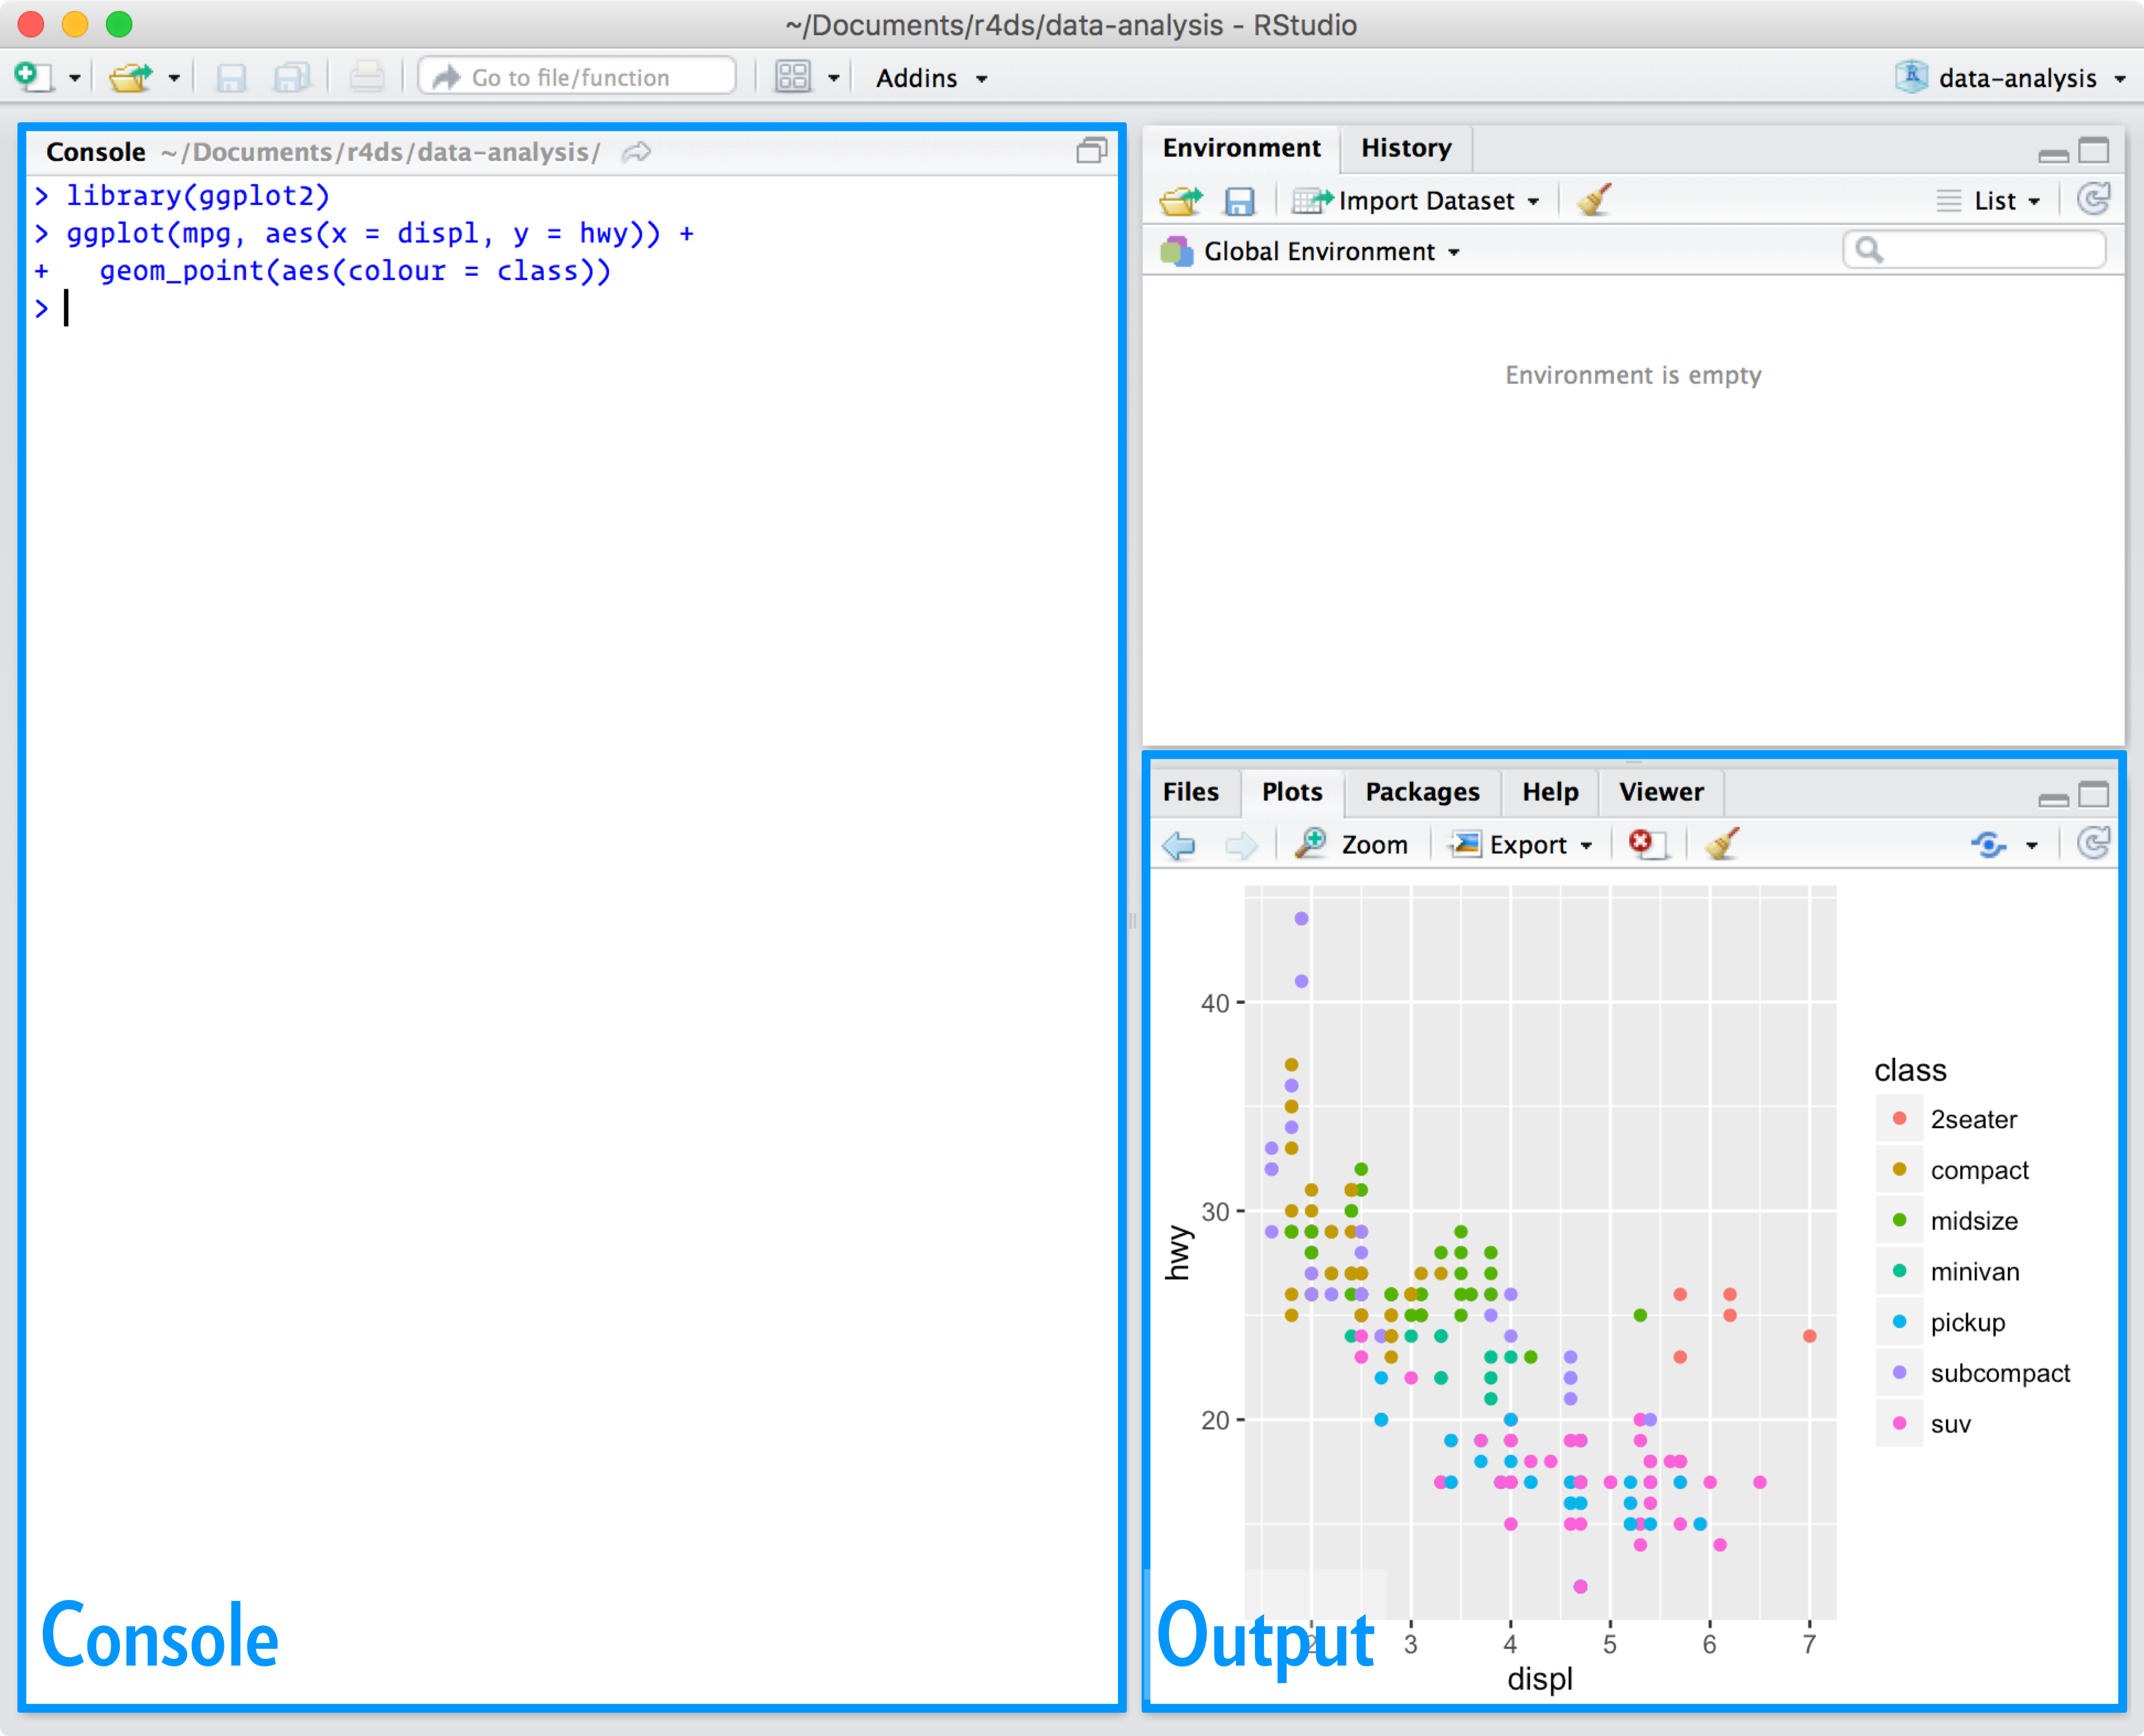
\includegraphics{images/rstudio.png}
\caption{Rstudio Windows}
\end{figure}

\subsection{Keyboard Shortcuts}\label{keyboard-shortcuts}

\begin{itemize}
\tightlist
\item
  \texttt{Ctrl+2}: move cursor to console
\item
  \texttt{Ctrl} (\texttt{Cmd} on Mac)\texttt{+Enter}: run current line
  (from editor) in console
\item
  \texttt{Ctrl} (\texttt{Cmd} on Mac)\texttt{+Enter}
\item
  \texttt{Uparrow}: retrieve recent commands in console
\item
  \texttt{Ctrl} (\texttt{Cmd} on Mac)\texttt{+Uparrow}: search previous
  commands
\item
  \texttt{Option\ -}: insert assignment operator (\texttt{\textless{}-})
\item
  \texttt{Ctrl} (\texttt{Cmd} on Mac)+\texttt{Shift+M}: insert pipe
  operator (\texttt{\%\textgreater{}\%})
\end{itemize}

\section{\texorpdfstring{Working Directory
(\texttt{wd})}{Working Directory (wd)}}\label{Working-directory}

\begin{itemize}
\tightlist
\item
  \emph{R} assumes a default (often inconvenient) working directory on
  your computer

  \begin{itemize}
  \tightlist
  \item
    this is where it thinks it will \textbf{load} any files you want to
    load and \textbf{save} anything you want to save by default
  \end{itemize}
\item
  Find out where \emph{R} currently thinks this is with
  \textbf{\texttt{getwd()}}

  \begin{itemize}
  \tightlist
  \item
    this is often Operating System specific, e.g.:

    \begin{itemize}
    \tightlist
    \item
      Mac: \texttt{/Users/yourusername/}
    \item
      Windows: \texttt{C:/Users/yourusername/Documents/}
    \end{itemize}
  \item
    you can move everything you want to load into this folder on your
    computer (and save everything there too), but this may be
    inconvenient
  \end{itemize}
\item
  \emph{Change} the working directory to wherever you plan on keeping
  your related data and documents with
  \textbf{\texttt{setwd("/path/to/folder")}}

  \begin{itemize}
  \tightlist
  \item
    you can move to a new \texttt{wd} \emph{relative} to the current
    working directory:

    \begin{itemize}
    \tightlist
    \item
      move down a folder by typing the folder name with a \texttt{/}
      after i

      \begin{itemize}
      \tightlist
      \item
        e.g.~to move from \texttt{/Ryansafner/Documents/} to
        \texttt{/Ryansafner/Documents/Econometrics/}
      \end{itemize}
    \item
      move up one folder in a hierarchy with \texttt{..}
    \item
      e.g.~to move from \texttt{/Ryansafner/Documents/} to
      \texttt{/Ryansafner/Downloads}, use
      \texttt{setwd("../Downloads/")} to move up from the
      \texttt{Documents} folder to \texttt{Ryansafner} folder, then down
      to Downloads
    \end{itemize}
  \end{itemize}
\end{itemize}

\section{Packages}\label{packages}

\begin{itemize}
\item
  \textbf{Packages} are extensions of base \texttt{R} designed by users

  \begin{itemize}
  \tightlist
  \item
    Remember, \texttt{R} is open source, packages are usually published
    first on \href{github.com}{Github}
  \item
    Official packages distributed and documented through
    \href{cran.r-project.org/}{CRAN}
  \end{itemize}
\item
  To use a (previously-installed) package (note the ``''), use the
  \texttt{library()} command:

\begin{verbatim}
library("packagename")
\end{verbatim}
\item
  If you do not have a package, they are easy to install with (note the
  plural ``s'')

\begin{verbatim}
install.packages("packagename")
\end{verbatim}
\item
  To install or load multiple packages at once, we can use the
  \texttt{c()} function to select multiple packages (\textbf{see below})
\end{itemize}

\begin{verbatim}
library(c("gapminder","ggplot2","dplyr"))
\end{verbatim}

\section{Useful Packages}\label{useful-packages}

\begin{itemize}
\tightlist
\item
  There are several packages we will use often (and are featured later
  in this guide)

  \begin{itemize}
  \tightlist
  \item
    Packages are often very well-documented with explanations and
    examples
  \item
    Google each package for more information
  \end{itemize}
\end{itemize}

\begin{table}
  \begin{tabular}{ll}
  Package name & Use \\ \toprule 
  \texttt{ggplot2} & Rendering beautiful graphics (scatterplots, histograms, etc)\\
  \texttt{stargazer} & Rendering professioanl looking regression output tables\\
  \texttt{dplyr} & Manipulating data much more intuitively\\
  \texttt{sandwich} & More tools for regression, particularly robust SE's\\
  \texttt{tidyverse} & An epic \emph{meta}package of \texttt{ggplot2, dplyr} and other popular packages\\ \bottomrule
  \end{tabular}
\end{table}

\section{Calculations}\label{calculations}

\begin{itemize}
\tightlist
\item
  \texttt{R} can be used as a calculator

  \begin{itemize}
  \tightlist
  \item
    Basic operations \texttt{+}, \texttt{-}, \texttt{*}, \texttt{/}
  \item
    More advanced math operators like exponents, logarithms,
    trigonometric functions, etc
  \end{itemize}
\end{itemize}

\begin{Shaded}
\begin{Highlighting}[]
\DecValTok{2}\OperatorTok{+}\DecValTok{2}
\end{Highlighting}
\end{Shaded}

\begin{verbatim}
## [1] 4
\end{verbatim}

\begin{Shaded}
\begin{Highlighting}[]
\DecValTok{6}\OperatorTok{^}\DecValTok{2} \CommentTok{# 6 to the second power (i.e. squared)}
\end{Highlighting}
\end{Shaded}

\begin{verbatim}
## [1] 36
\end{verbatim}

\begin{Shaded}
\begin{Highlighting}[]
\KeywordTok{sqrt}\NormalTok{(}\DecValTok{100}\OperatorTok{/}\DecValTok{4}\NormalTok{) }\CommentTok{# square root }
\end{Highlighting}
\end{Shaded}

\begin{verbatim}
## [1] 5
\end{verbatim}

\begin{Shaded}
\begin{Highlighting}[]
\KeywordTok{log}\NormalTok{(}\DecValTok{5}\NormalTok{) }\CommentTok{# logarithm}
\end{Highlighting}
\end{Shaded}

\begin{verbatim}
## [1] 1.609438
\end{verbatim}

\begin{Shaded}
\begin{Highlighting}[]
\KeywordTok{sin}\NormalTok{(}\DecValTok{2}\OperatorTok{*}\NormalTok{pi) }\CommentTok{# sin}
\end{Highlighting}
\end{Shaded}

\begin{verbatim}
## [1] -2.449294e-16
\end{verbatim}

\begin{Shaded}
\begin{Highlighting}[]
\KeywordTok{factorial}\NormalTok{(}\DecValTok{5}\NormalTok{) }\CommentTok{# factorial (e.g. 5!)}
\end{Highlighting}
\end{Shaded}

\begin{verbatim}
## [1] 120
\end{verbatim}

\begin{Shaded}
\begin{Highlighting}[]
\KeywordTok{choose}\NormalTok{(}\DecValTok{2}\NormalTok{,}\DecValTok{6}\NormalTok{) }\CommentTok{# binomial choose function}
\end{Highlighting}
\end{Shaded}

\begin{verbatim}
## [1] 0
\end{verbatim}

\begin{Shaded}
\begin{Highlighting}[]
\CommentTok{# order of operations matters}
\DecValTok{3}\OperatorTok{*}\DecValTok{3}\OperatorTok{+}\DecValTok{4}
\end{Highlighting}
\end{Shaded}

\begin{verbatim}
## [1] 13
\end{verbatim}

\begin{Shaded}
\begin{Highlighting}[]
\DecValTok{3}\OperatorTok{*}\NormalTok{(}\DecValTok{3}\OperatorTok{+}\DecValTok{4}\NormalTok{)}
\end{Highlighting}
\end{Shaded}

\begin{verbatim}
## [1] 21
\end{verbatim}

\begin{itemize}
\tightlist
\item
  \textbf{Note on Notation}: \texttt{R} often reports very large (or
  very small) numbers in scientific notation with \texttt{e}

  \begin{itemize}
  \tightlist
  \item
    For positive \texttt{e}: the number of zeros (or digits after the
    decimal point) to the right of a number

    \begin{itemize}
    \tightlist
    \item
      e.g. \(1.25e6 = 1.25 \times 10^6 = 1,250,000\)
    \end{itemize}
  \item
    For negative \texttt{e}: one less than the number of zeros (or
    digits after the decimal point) to the left of a number

    \begin{itemize}
    \tightlist
    \item
      e.g. \(1.25e-6 = 1.25 \times 10^{-6} = 0.00000125\)
    \end{itemize}
  \end{itemize}
\end{itemize}

\section{Hints for Writing Code}\label{hints-for-writing-code}

\subsection{Naming Objects}\label{naming-objects}

\begin{itemize}
\item
  Object names cannot start with a digit or contain a space or comma
\item
  FOR THE LOVE OF GOD AVOID SPACES IN GENERAL

  \begin{itemize}
  \tightlist
  \item
    You've seen webpages intended to be called
    \texttt{"my\ webpage\ in\ html"} turned into
    \texttt{http://my\%20webpage\%20in\%20html.html}
  \item
    Consider both your \texttt{R} objects and your files and folder
    names on your
    computer\ldots{}(\texttt{/School/ECON\_480\_Econometrics/Homeworks\_and\_Data/})
  \end{itemize}
\item
  It will be wise to adopt some consistent standard for demarcating
  names:

\begin{verbatim}
i.use.snake.case
otherPeopleUseCamelCase
some_people_use_underscores
And_aFew.People_RENOUNCEconvention
\end{verbatim}
\end{itemize}

\subsection{Commenting}\label{commenting}

\begin{itemize}
\tightlist
\item
  Always comment your commands! Describe what you are doing so someone
  else (or you, 5 years later) can understand what is happening and why!

  \begin{itemize}
  \tightlist
  \item
    Use the hashtag \texttt{\#} to start a comment (\texttt{R} ignores
    everything on that line after the hashtag)
  \item
    Can be made its own line or at the end of lines
  \item
    e.g.
  \end{itemize}
\end{itemize}

\begin{Shaded}
\begin{Highlighting}[]
\CommentTok{# Run regression of y on x, save as reg1}
\NormalTok{reg1<-}\KeywordTok{lm}\NormalTok{(y}\OperatorTok{~}\NormalTok{x, }\DataTypeTok{data=}\NormalTok{mydata) }\CommentTok{# runs regression using mydata }
\KeywordTok{summary}\NormalTok{(reg1}\OperatorTok{$}\NormalTok{coefficients) }\CommentTok{# prints coefficients}
\end{Highlighting}
\end{Shaded}

\subsection{Managing Your Workflow}\label{managing-your-workflow}

\begin{itemize}
\tightlist
\item
  \textbf{Save often!}

  \begin{itemize}
  \tightlist
  \item
    Better yet, ask me about version control and GitHub
  \end{itemize}
\end{itemize}

\section{Getting Help}\label{getting-help}

\begin{itemize}
\tightlist
\item
  You can get documentation, explanations, and examples of every command
  in \texttt{R}

  \begin{itemize}
  \tightlist
  \item
    simply type \texttt{?commandname} or \texttt{help("commandname")}
  \end{itemize}
\item
  Meet your new friend:
\end{itemize}

\begin{figure}
\centering

\includegraphics{images/googlehelp.png}
\caption{}
\end{figure}

\begin{itemize}
\tightlist
\item
  Meet your new \emph{best} friend:
\end{itemize}

\begin{figure}
\centering
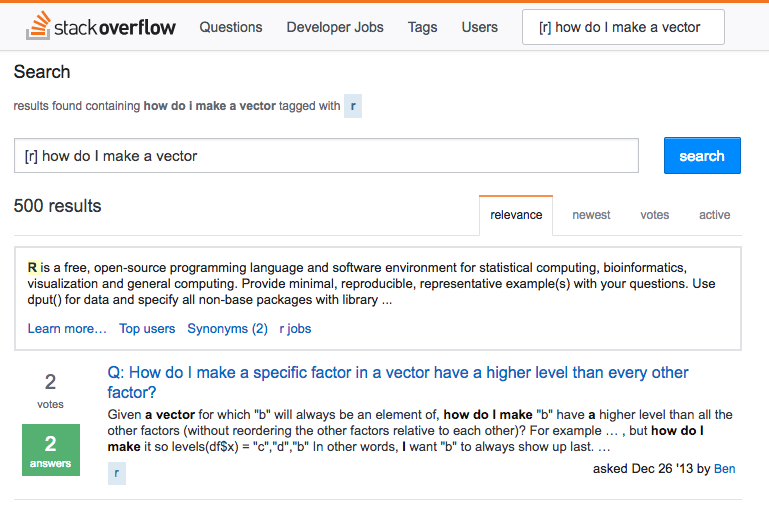
\includegraphics{images/stackoverflow.png}
\caption{}
\end{figure}

\begin{itemize}
\tightlist
\item
  The \textbf{only} way to learn coding is by tweaking existing
  examples, messing up, and searching the internet for help!
\end{itemize}

\chapter{\texorpdfstring{\texttt{R}
Objects}{R Objects}}\label{r-objects}

\texttt{R} is an \textbf{object-oriented} programming language, meaning
we will almost always store data in \textbf{objects} and run
\textbf{functions} on those objects. We \textbf{assign} values to
objects using the \textbf{assignment operator
(\texttt{\textless{}-})}\footnote{Think of the assignment operator like
  like an \(=\) sign, but we want to avoid using the equals sign.
  \texttt{\textless{}-} was
  \href{https://twitter.com/kwbroman/status/747829864091127809}{originally
  its own key} on early computer keyboards.}

\begin{Shaded}
\begin{Highlighting}[]
\NormalTok{myobject<-value}
\end{Highlighting}
\end{Shaded}

The keyboard shortcut for inserting \texttt{\textless{}-} (inside the
Console or an \texttt{R} chunk) is \texttt{Alt}+\texttt{-} (on Windows)
or \texttt{Option}+\texttt{-} (on Mac).

\textbf{Functions} take the form:

\begin{Shaded}
\begin{Highlighting}[]
\KeywordTok{functionname}\NormalTok{(myobject)}
\end{Highlighting}
\end{Shaded}

Functions can have \emph{other} functions for \textbf{arguments} (the
object the function is run on), e.g.

\begin{Shaded}
\begin{Highlighting}[]
\KeywordTok{round}\NormalTok{(}\KeywordTok{rnorm}\NormalTok{(}\DecValTok{5}\NormalTok{),}\DecValTok{2}\NormalTok{) }
\CommentTok{# rnorm(5) takes 5 random draws from a normal distribution}
\CommentTok{# then round(, 2) rounds the result to 2 decimal places}
\end{Highlighting}
\end{Shaded}

\section{Vectors}\label{vectors}

The simplest data structure in \texttt{R} is a \textbf{vector}, simply a
collection of objects or elements. To construct a vector, use the
``combine/concatenate'' function ``\texttt{c()}''

As an example, let's make a vector of the numbers 1 through 5, called
\texttt{v}.

\begin{Shaded}
\begin{Highlighting}[]
\NormalTok{v<-}\KeywordTok{c}\NormalTok{(}\DecValTok{1}\NormalTok{,}\DecValTok{2}\NormalTok{,}\DecValTok{3}\NormalTok{,}\DecValTok{4}\NormalTok{,}\DecValTok{5}\NormalTok{)}
\end{Highlighting}
\end{Shaded}

We can also build vectors via generating mathematical \textbf{series}
with the \texttt{:} operator, which lists all integers in a series from
\texttt{beginning:end}.

\begin{Shaded}
\begin{Highlighting}[]
\NormalTok{v<-}\DecValTok{1}\OperatorTok{:}\DecValTok{5}
\end{Highlighting}
\end{Shaded}

To inspect an object, we simply ``call'' it up by typing the name of the
object to print its contents.

\begin{Shaded}
\begin{Highlighting}[]
\NormalTok{v}
\end{Highlighting}
\end{Shaded}

\begin{verbatim}
## [1] 1 2 3 4 5
\end{verbatim}

\subsection{Functions}\label{functions}

Since a vector is an object, we can run functions on that object. Let's
start with some simple mathematical functions, such as taking the sum
and taking the mean of our simple vector \texttt{v}.

\begin{Shaded}
\begin{Highlighting}[]
\KeywordTok{sum}\NormalTok{(v)}
\end{Highlighting}
\end{Shaded}

\begin{verbatim}
## [1] 15
\end{verbatim}

\begin{Shaded}
\begin{Highlighting}[]
\KeywordTok{mean}\NormalTok{(v)}
\end{Highlighting}
\end{Shaded}

\begin{verbatim}
## [1] 3
\end{verbatim}

Functions in \texttt{R} are ``vectorized,'' meaning the function is run
on every object inside a vector.

We can perform mathematical operations on a vector as a whole:

\begin{Shaded}
\begin{Highlighting}[]
\KeywordTok{sum}\NormalTok{(}\DecValTok{1}\OperatorTok{:}\DecValTok{5}\NormalTok{)}
\end{Highlighting}
\end{Shaded}

\begin{verbatim}
## [1] 15
\end{verbatim}

\begin{Shaded}
\begin{Highlighting}[]
\KeywordTok{mean}\NormalTok{(}\DecValTok{1}\OperatorTok{:}\DecValTok{5}\NormalTok{)}
\end{Highlighting}
\end{Shaded}

\begin{verbatim}
## [1] 3
\end{verbatim}

\section{Other Object Types}\label{other-object-types}

\subsection{Lists}\label{lists}

\begin{itemize}
\tightlist
\item
  A \textbf{list} is a non-atomic vector, meaning you can gather data
  elements of different classes in one object
\end{itemize}

\begin{Shaded}
\begin{Highlighting}[]
\NormalTok{mylist<-}\KeywordTok{list}\NormalTok{(}\DecValTok{5}\NormalTok{, pi, }\OtherTok{TRUE}\NormalTok{, }\FloatTok{4.3}\NormalTok{, }\StringTok{"cabbage"}\NormalTok{)}
\KeywordTok{class}\NormalTok{(mylist)}
\end{Highlighting}
\end{Shaded}

\begin{verbatim}
## [1] "list"
\end{verbatim}

\begin{itemize}
\tightlist
\item
  Another great property of lists is that elements of the list can
  themselves be vectors
\end{itemize}

\begin{Shaded}
\begin{Highlighting}[]
\NormalTok{vectored.list<-}\KeywordTok{list}\NormalTok{(}\KeywordTok{c}\NormalTok{(}\FloatTok{1.82}\NormalTok{, }\DecValTok{1940}\NormalTok{, }\FloatTok{93.20}\NormalTok{, }\FloatTok{192.917}\NormalTok{),}
     \KeywordTok{c}\NormalTok{(}\StringTok{"Orange"}\NormalTok{, }\StringTok{"Cyan"}\NormalTok{, }\StringTok{"Pink"}\NormalTok{),}
     \KeywordTok{c}\NormalTok{(}\OtherTok{TRUE}\NormalTok{, }\OtherTok{FALSE}\NormalTok{, }\OtherTok{TRUE}\NormalTok{, }\OtherTok{TRUE}\NormalTok{, }\OtherTok{FALSE}\NormalTok{, }\OtherTok{TRUE}\NormalTok{, }\OtherTok{FALSE}\NormalTok{, }\OtherTok{FALSE}\NormalTok{))}

\KeywordTok{str}\NormalTok{(vectored.list) }\CommentTok{# look at structure of the list}
\end{Highlighting}
\end{Shaded}

\begin{verbatim}
## List of 3
##  $ : num [1:4] 1.82 1940 93.2 192.92
##  $ : chr [1:3] "Orange" "Cyan" "Pink"
##  $ : logi [1:8] TRUE FALSE TRUE TRUE FALSE TRUE ...
\end{verbatim}

\begin{itemize}
\tightlist
\item
  We can create a \textbf{label} for each element in a list, called a
  \texttt{name}
\end{itemize}

\begin{Shaded}
\begin{Highlighting}[]
\NormalTok{vectored.list<-}\KeywordTok{list}\NormalTok{(}\DataTypeTok{numbers=}\KeywordTok{c}\NormalTok{(}\FloatTok{1.82}\NormalTok{, }\DecValTok{1940}\NormalTok{, }\FloatTok{93.20}\NormalTok{, }\FloatTok{192.917}\NormalTok{), }\CommentTok{# first element is a vector called 'numbers'}
     \DataTypeTok{colors=}\KeywordTok{c}\NormalTok{(}\StringTok{"Orange"}\NormalTok{, }\StringTok{"Cyan"}\NormalTok{, }\StringTok{"Pink"}\NormalTok{), }\CommentTok{# second element is a vector called `colors`}
     \DataTypeTok{logic=}\KeywordTok{c}\NormalTok{(}\OtherTok{TRUE}\NormalTok{, }\OtherTok{FALSE}\NormalTok{, }\OtherTok{TRUE}\NormalTok{, }\OtherTok{TRUE}\NormalTok{, }\OtherTok{FALSE}\NormalTok{, }\OtherTok{TRUE}\NormalTok{, }\OtherTok{FALSE}\NormalTok{, }\OtherTok{FALSE}\NormalTok{)) }\CommentTok{# third element is a vector called `logic`}

\NormalTok{vectored.list}
\end{Highlighting}
\end{Shaded}

\begin{verbatim}
## $numbers
## [1]    1.820 1940.000   93.200  192.917
## 
## $colors
## [1] "Orange" "Cyan"   "Pink"  
## 
## $logic
## [1]  TRUE FALSE  TRUE  TRUE FALSE  TRUE FALSE FALSE
\end{verbatim}

\begin{itemize}
\tightlist
\item
  The \texttt{names} command prints (or changes) the name of the label
  of each element in the list
\end{itemize}

\begin{Shaded}
\begin{Highlighting}[]
\KeywordTok{names}\NormalTok{(vectored.list) }\CommentTok{# print the names of the list elements}
\end{Highlighting}
\end{Shaded}

\begin{verbatim}
## [1] "numbers" "colors"  "logic"
\end{verbatim}

\begin{Shaded}
\begin{Highlighting}[]
\KeywordTok{names}\NormalTok{(vectored.list)<-}\KeywordTok{c}\NormalTok{(}\StringTok{"name1"}\NormalTok{,}\StringTok{"name2"}\NormalTok{,}\StringTok{"name3"}\NormalTok{) }\CommentTok{# rename the lables to 'name1', 'name2', and 'name3'}

\KeywordTok{names}\NormalTok{(vectored.list) }\CommentTok{# print new names}
\end{Highlighting}
\end{Shaded}

\begin{verbatim}
## [1] "name1" "name2" "name3"
\end{verbatim}

\begin{Shaded}
\begin{Highlighting}[]
\NormalTok{vectored.list }\CommentTok{# print list with new names}
\end{Highlighting}
\end{Shaded}

\begin{verbatim}
## $name1
## [1]    1.820 1940.000   93.200  192.917
## 
## $name2
## [1] "Orange" "Cyan"   "Pink"  
## 
## $name3
## [1]  TRUE FALSE  TRUE  TRUE FALSE  TRUE FALSE FALSE
\end{verbatim}

\subsection{Matrix}\label{matrix}

\begin{itemize}
\tightlist
\item
  Everything thus far has been 1 dimension, but we often work with
  2-dimensional data

  \begin{itemize}
  \tightlist
  \item
    Rows are observations
  \item
    Columns are variables
  \end{itemize}
\item
  A \textbf{matrix}

  \begin{itemize}
  \tightlist
  \item
    \texttt{matrix()} command creates a matrix by column,

    \begin{itemize}
    \tightlist
    \item
      can define number of rows with \texttt{nrow=}, \texttt{R} will
      divide the elements into equal number of columns
    \end{itemize}
  \end{itemize}
\end{itemize}

\begin{Shaded}
\begin{Highlighting}[]
\NormalTok{matrix1<-}\KeywordTok{matrix}\NormalTok{(}\KeywordTok{c}\NormalTok{(}\DecValTok{1}\NormalTok{,}\DecValTok{2}\NormalTok{,}\DecValTok{3}\NormalTok{,}\DecValTok{4}\NormalTok{,}\DecValTok{5}\NormalTok{,}\DecValTok{6}\NormalTok{),}\DataTypeTok{nrow=}\DecValTok{3}\NormalTok{) }\CommentTok{# make a 3-row matrix}
\NormalTok{matrix1 }
\end{Highlighting}
\end{Shaded}

\begin{verbatim}
##      [,1] [,2]
## [1,]    1    4
## [2,]    2    5
## [3,]    3    6
\end{verbatim}

\subsection{Data Frame}\label{data-frame}

\begin{itemize}
\tightlist
\item
  The most important object in \texttt{R} is a \textbf{data frame} (what
  you call a ``spreadsheet''), used for statistics, plots, regressions,
  etc

  \begin{itemize}
  \tightlist
  \item
    ``Rectangular'' data, rows are observations, columns are variables
  \item
    Can hold variables of different classes (e.g.~a quantitative
    variable like income, a character variable like name, etc)
  \item
    In essence, data frames are actually lists (where each list object
    itself is a vector)
  \item
    All vectors (columns) must have the same length!
  \end{itemize}
\end{itemize}

\begin{Shaded}
\begin{Highlighting}[]
\NormalTok{df<-}\KeywordTok{data.frame}\NormalTok{(}\DataTypeTok{x =} \DecValTok{1}\OperatorTok{:}\DecValTok{3}\NormalTok{,}
           \DataTypeTok{y =} \KeywordTok{c}\NormalTok{(}\StringTok{"a"}\NormalTok{, }\StringTok{"b"}\NormalTok{, }\StringTok{"c"}\NormalTok{),}
           \DataTypeTok{z =} \KeywordTok{c}\NormalTok{(}\OtherTok{TRUE}\NormalTok{, }\OtherTok{FALSE}\NormalTok{, }\OtherTok{TRUE}\NormalTok{))}
\NormalTok{df}
\end{Highlighting}
\end{Shaded}

\begin{verbatim}
##   x y     z
## 1 1 a  TRUE
## 2 2 b FALSE
## 3 3 c  TRUE
\end{verbatim}

\section{Data Classes}\label{data-classes}

\begin{itemize}
\tightlist
\item
  Vectors \textbf{must} contain the same type of elements
  (e.g.~numerical or text)
\item
  Technically this refers to \textbf{atomic vectors} (nearly all vectors
  are atomic)
\item
  Vectors with ``mixed'' types will convert all elements to the
  lowest-common denominator, e.g.~character
\item
  You can always check the type of vector using \textbf{class()}
\end{itemize}

\begin{Shaded}
\begin{Highlighting}[]
\NormalTok{mixed<-}\KeywordTok{c}\NormalTok{(}\DecValTok{5}\NormalTok{, pi, }\OtherTok{TRUE}\NormalTok{, }\FloatTok{4.3}\NormalTok{, }\StringTok{"cabbage"}\NormalTok{)}
\KeywordTok{class}\NormalTok{(mixed)}
\end{Highlighting}
\end{Shaded}

\begin{verbatim}
## [1] "character"
\end{verbatim}

\subsection{Numeric}\label{numeric}

\begin{itemize}
\tightlist
\item
  \textbf{Numeric} (aka ``double''), as it sounds, can perform
  mathematical operations
\end{itemize}

\begin{Shaded}
\begin{Highlighting}[]
\NormalTok{numeric<-}\KeywordTok{c}\NormalTok{(}\DecValTok{1}\NormalTok{,}\DecValTok{2}\NormalTok{,}\DecValTok{3}\NormalTok{,}\DecValTok{4}\NormalTok{,}\DecValTok{5}\NormalTok{)}
\end{Highlighting}
\end{Shaded}

\begin{itemize}
\tightlist
\item
  There are two \textbf{types} of numeric objects: \textbf{double} and
  \textbf{integer}
\end{itemize}

\subsection{Double}\label{double}

\begin{itemize}
\tightlist
\item
  If numeric values contain decimal points, they are technically called
  \textbf{floating point double} or simply \textbf{double} class
\item
  \texttt{R} may simply call them numeric, but contrast with integer
  below
\end{itemize}

\begin{Shaded}
\begin{Highlighting}[]
\NormalTok{double<-}\KeywordTok{c}\NormalTok{(pi,}\FloatTok{2.34}\NormalTok{,}\FloatTok{9.99}\NormalTok{)}

\KeywordTok{class}\NormalTok{(double)}
\end{Highlighting}
\end{Shaded}

\begin{verbatim}
## [1] "numeric"
\end{verbatim}

\begin{Shaded}
\begin{Highlighting}[]
\KeywordTok{typeof}\NormalTok{(double) }\CommentTok{# will return the more specific type }
\end{Highlighting}
\end{Shaded}

\begin{verbatim}
## [1] "double"
\end{verbatim}

\begin{Shaded}
\begin{Highlighting}[]
\KeywordTok{is.double}\NormalTok{(double) }\CommentTok{# a logical test to see if object is "double" type}
\end{Highlighting}
\end{Shaded}

\begin{verbatim}
## [1] TRUE
\end{verbatim}

\begin{Shaded}
\begin{Highlighting}[]
\KeywordTok{is.integer}\NormalTok{(double) }\CommentTok{# a logical test to see if object is "integer" type}
\end{Highlighting}
\end{Shaded}

\begin{verbatim}
## [1] FALSE
\end{verbatim}

\subsubsection{Integer}\label{integer}

\begin{itemize}
\tightlist
\item
  If numeric values are all whole numbers, they are \textbf{integer}
  class
\end{itemize}

\begin{Shaded}
\begin{Highlighting}[]
\NormalTok{integers<-}\KeywordTok{c}\NormalTok{(}\DecValTok{1}\NormalTok{,}\DecValTok{2}\NormalTok{,}\DecValTok{3}\NormalTok{,}\DecValTok{4}\NormalTok{)}
\KeywordTok{class}\NormalTok{(integers)}
\end{Highlighting}
\end{Shaded}

\begin{verbatim}
## [1] "numeric"
\end{verbatim}

\begin{Shaded}
\begin{Highlighting}[]
\KeywordTok{typeof}\NormalTok{(integers)}
\end{Highlighting}
\end{Shaded}

\begin{verbatim}
## [1] "double"
\end{verbatim}

\begin{Shaded}
\begin{Highlighting}[]
\KeywordTok{is.double}\NormalTok{(double)}
\end{Highlighting}
\end{Shaded}

\begin{verbatim}
## [1] TRUE
\end{verbatim}

\begin{Shaded}
\begin{Highlighting}[]
\KeywordTok{is.integer}\NormalTok{(double)}
\end{Highlighting}
\end{Shaded}

\begin{verbatim}
## [1] FALSE
\end{verbatim}

\subsection{Logical}\label{logical}

\begin{itemize}
\tightlist
\item
  \textbf{Logical} is a series of binary elements or statements that can
  either be TRUE or FALSE
\end{itemize}

\begin{Shaded}
\begin{Highlighting}[]
\NormalTok{logical<-}\KeywordTok{c}\NormalTok{(}\OtherTok{TRUE}\NormalTok{,}\OtherTok{FALSE}\NormalTok{,}\OtherTok{FALSE}\NormalTok{,}\OtherTok{TRUE}\NormalTok{)}
\end{Highlighting}
\end{Shaded}

\begin{itemize}
\tightlist
\item
  We can perform logical tests with common operators:

  \begin{itemize}
  \tightlist
  \item
    \texttt{\textless{}} less than
  \item
    \texttt{\textgreater{}} greater than
  \item
    \texttt{\textless{}=} less than or equal to (\(\leq\))
  \item
    \texttt{\textgreater{}=} greater than or equal to (\(\geq\))
  \item
    \texttt{==} is equal to (note two equals signs are needed!)
  \item
    \texttt{!=} is not equal to
  \item
    \texttt{\%in\%} is a member of a set (\(\in\))
  \end{itemize}
\end{itemize}

\begin{Shaded}
\begin{Highlighting}[]
\DecValTok{3}\OperatorTok{==}\DecValTok{4} \CommentTok{#is 3 equal to 4?}
\end{Highlighting}
\end{Shaded}

\begin{verbatim}
## [1] FALSE
\end{verbatim}

\begin{Shaded}
\begin{Highlighting}[]
\DecValTok{3}\OperatorTok{<}\DecValTok{4} \CommentTok{# is three less than 4?}
\end{Highlighting}
\end{Shaded}

\begin{verbatim}
## [1] TRUE
\end{verbatim}

\begin{Shaded}
\begin{Highlighting}[]
\DecValTok{3}\OperatorTok{<=}\DecValTok{4} \CommentTok{# is three less than or equal to 4?}
\end{Highlighting}
\end{Shaded}

\begin{verbatim}
## [1] TRUE
\end{verbatim}

\begin{Shaded}
\begin{Highlighting}[]
\DecValTok{3}\OperatorTok{>}\DecValTok{4} \CommentTok{# is three greater than 4?}
\end{Highlighting}
\end{Shaded}

\begin{verbatim}
## [1] FALSE
\end{verbatim}

\begin{Shaded}
\begin{Highlighting}[]
\DecValTok{3}\OperatorTok{!=}\DecValTok{4} \CommentTok{# is three not equal to four?}
\end{Highlighting}
\end{Shaded}

\begin{verbatim}
## [1] TRUE
\end{verbatim}

\begin{Shaded}
\begin{Highlighting}[]
\DecValTok{3} \OperatorTok\StringTok{ }\KeywordTok{c}\NormalTok{(}\DecValTok{0}\NormalTok{,}\DecValTok{1}\NormalTok{,}\DecValTok{2}\NormalTok{) }\CommentTok{# is three in the following set of numbers?}
\end{Highlighting}
\end{Shaded}

\begin{verbatim}
## [1] FALSE
\end{verbatim}

\begin{Shaded}
\begin{Highlighting}[]
\DecValTok{3} \OperatorTok\StringTok{ }\KeywordTok{c}\NormalTok{(}\DecValTok{0}\NormalTok{,}\DecValTok{1}\NormalTok{,}\DecValTok{2}\NormalTok{,}\DecValTok{3}\NormalTok{) }\CommentTok{# is three in the following set of numbers?}
\end{Highlighting}
\end{Shaded}

\begin{verbatim}
## [1] TRUE
\end{verbatim}

\begin{itemize}
\tightlist
\item
  We are not limited to using numeric data, \texttt{R} can also perform
  logical tests on other classes of variable, like characters (which
  need quotes):
\end{itemize}

\begin{Shaded}
\begin{Highlighting}[]
\StringTok{"red"}\OperatorTok{==}\StringTok{"blue"} \CommentTok{# is red the same as blue?}
\end{Highlighting}
\end{Shaded}

\begin{verbatim}
## [1] FALSE
\end{verbatim}

\begin{Shaded}
\begin{Highlighting}[]
\StringTok{"red"}\OperatorTok{!=}\StringTok{"blue"} \CommentTok{# is red not equal to blue?}
\end{Highlighting}
\end{Shaded}

\begin{verbatim}
## [1] TRUE
\end{verbatim}

\begin{Shaded}
\begin{Highlighting}[]
\NormalTok{political.party<-}\KeywordTok{c}\NormalTok{(}\StringTok{"Republican"}\NormalTok{,}\StringTok{"Democrat"}\NormalTok{) }\CommentTok{# define political party as a set of Republican and Democrat}
\StringTok{"Libertarian"} \OperatorTok\StringTok{ }\NormalTok{political.party }\CommentTok{# check if Libertarian is in the set of political parties we created}
\end{Highlighting}
\end{Shaded}

\begin{verbatim}
## [1] FALSE
\end{verbatim}

\begin{Shaded}
\begin{Highlighting}[]
\StringTok{"Democrat"} \OperatorTok\StringTok{ }\NormalTok{political.party }\CommentTok{# check if Democrat is in our set of political parties }
\end{Highlighting}
\end{Shaded}

\begin{verbatim}
## [1] TRUE
\end{verbatim}

\begin{itemize}
\tightlist
\item
  We can also perform more than one test at a time with multiple
  conditions:

  \begin{itemize}
  \tightlist
  \item
    \texttt{\&} AND
  \item
    \texttt{\textbar{}} OR
  \end{itemize}
\end{itemize}

\begin{Shaded}
\begin{Highlighting}[]
\DecValTok{2}\OperatorTok{==}\DecValTok{2} \OperatorTok{&}\StringTok{ }\DecValTok{2}\OperatorTok{>}\DecValTok{3} \CommentTok{# is 2 equal to 2 AND greater than 3? }
\end{Highlighting}
\end{Shaded}

\begin{verbatim}
## [1] FALSE
\end{verbatim}

\begin{Shaded}
\begin{Highlighting}[]
\DecValTok{2}\OperatorTok{==}\DecValTok{2} \OperatorTok{|}\StringTok{ }\DecValTok{2}\OperatorTok{>}\DecValTok{3} \CommentTok{# is 2 equal to 2 OR greater than 3? }
\end{Highlighting}
\end{Shaded}

\begin{verbatim}
## [1] TRUE
\end{verbatim}

\begin{itemize}
\tightlist
\item
  These commands will become very useful when we want to subset data or
  look at portions of our data based on some condition
\end{itemize}

\subsection{Character}\label{character}

\begin{itemize}
\tightlist
\item
  \textbf{Character} is a string of text: letters, numbers, and symbols,
  cannot perform mathematical operations

  \begin{itemize}
  \tightlist
  \item
    Character values require quotation marks around each value
  \end{itemize}
\end{itemize}

\begin{Shaded}
\begin{Highlighting}[]
\NormalTok{character<-}\KeywordTok{c}\NormalTok{(}\StringTok{"one"}\NormalTok{,}\StringTok{"two"}\NormalTok{,}\StringTok{"7"}\NormalTok{,}\StringTok{"orange"}\NormalTok{)}
\end{Highlighting}
\end{Shaded}

\subsubsection{Dates}\label{dates}

\begin{itemize}
\tightlist
\item
  Dates are a specific type of character class
\item
  Specific dates

  \begin{itemize}
  \tightlist
  \item
    Can do days, weeks, months, quarters, years
  \end{itemize}
\end{itemize}

\begin{Shaded}
\begin{Highlighting}[]
\NormalTok{today<-}\KeywordTok{Sys.Date}\NormalTok{() }\CommentTok{#print today's date }
\KeywordTok{format}\NormalTok{(today, }\DataTypeTok{format=}\StringTok{"%B %d %Y"}\NormalTok{) }\CommentTok{# specify how to report date format }
\end{Highlighting}
\end{Shaded}

\begin{verbatim}
## [1] "December 18 2018"
\end{verbatim}

\begin{Shaded}
\begin{Highlighting}[]
\NormalTok{months<-}\KeywordTok{seq}\NormalTok{(}\KeywordTok{as.Date}\NormalTok{(}\StringTok{"2010/1/1"}\NormalTok{), }\KeywordTok{as.Date}\NormalTok{(}\StringTok{"2012/1/1"}\NormalTok{), }\StringTok{"months"}\NormalTok{) }\CommentTok{# generate sequence of months between Jan 2010 and Jan 2012}
\NormalTok{months}
\end{Highlighting}
\end{Shaded}

\begin{verbatim}
##  [1] "2010-01-01" "2010-02-01" "2010-03-01" "2010-04-01" "2010-05-01"
##  [6] "2010-06-01" "2010-07-01" "2010-08-01" "2010-09-01" "2010-10-01"
## [11] "2010-11-01" "2010-12-01" "2011-01-01" "2011-02-01" "2011-03-01"
## [16] "2011-04-01" "2011-05-01" "2011-06-01" "2011-07-01" "2011-08-01"
## [21] "2011-09-01" "2011-10-01" "2011-11-01" "2011-12-01" "2012-01-01"
\end{verbatim}

\subsection{Factor}\label{factor}

\begin{itemize}
\tightlist
\item
  \textbf{Factor} is a special type of character variable, often used to
  indicate membership in one of several possible categories, called
  \textbf{levels} (e.g.~for plotting, or conditional statistics and data
  work)
\end{itemize}

\begin{Shaded}
\begin{Highlighting}[]
\NormalTok{students<-}\KeywordTok{factor}\NormalTok{(}\KeywordTok{c}\NormalTok{(}\StringTok{"freshman"}\NormalTok{, }\StringTok{"senior"}\NormalTok{, }\StringTok{"senior"}\NormalTok{, }\StringTok{"junior"}\NormalTok{, }\StringTok{"freshman"}\NormalTok{, }
                   \StringTok{"sophomore"}\NormalTok{, }\StringTok{"freshman"}\NormalTok{))}
\NormalTok{students }\CommentTok{# note order is arbitrary}
\end{Highlighting}
\end{Shaded}

\begin{verbatim}
## [1] freshman  senior    senior    junior    freshman  sophomore freshman 
## Levels: freshman junior senior sophomore
\end{verbatim}

\begin{Shaded}
\begin{Highlighting}[]
\KeywordTok{levels}\NormalTok{(students) }\CommentTok{#extract unique levels }
\end{Highlighting}
\end{Shaded}

\begin{verbatim}
## [1] "freshman"  "junior"    "senior"    "sophomore"
\end{verbatim}

\begin{Shaded}
\begin{Highlighting}[]
\KeywordTok{nlevels}\NormalTok{(students) }\CommentTok{#count the number of levels }
\end{Highlighting}
\end{Shaded}

\begin{verbatim}
## [1] 4
\end{verbatim}

\begin{Shaded}
\begin{Highlighting}[]
\KeywordTok{table}\NormalTok{(students) }\CommentTok{#tabulate number of values for each level }
\end{Highlighting}
\end{Shaded}

\begin{verbatim}
## students
##  freshman    junior    senior sophomore 
##         3         1         2         1
\end{verbatim}

\subsubsection{Ordered Factors}\label{ordered-factors}

\begin{itemize}
\tightlist
\item
  Factors have ordered \texttt{levels()} which control the order on
  plots and in \texttt{table()}
\end{itemize}

\begin{Shaded}
\begin{Highlighting}[]
\NormalTok{students.o<-}\KeywordTok{ordered}\NormalTok{(students, }\DataTypeTok{levels=}\KeywordTok{c}\NormalTok{(}\StringTok{"freshman"}\NormalTok{,}\StringTok{"sophomore"}\NormalTok{,}\StringTok{"junior"}\NormalTok{,}\StringTok{"senior"}\NormalTok{))}
\NormalTok{students.o}
\end{Highlighting}
\end{Shaded}

\begin{verbatim}
## [1] freshman  senior    senior    junior    freshman  sophomore freshman 
## Levels: freshman < sophomore < junior < senior
\end{verbatim}

\begin{itemize}
\tightlist
\item
  \textbf{Be advised}: when \texttt{R} stores and calls factors, it
  actually stores them as integers {[}1..k, for k categories{]} instead
  of characters (e.g. ``freshman''=1, ``sophomore''=2), making this a
  \textbf{nominal} variable. This allows for some mathematical
  operations.
\item
  An \textbf{ordered factor} is where the ordering matters (e.g.
  ``small'', ``medium'', ``large'' coded as 1, 2, 3 in order)
\end{itemize}

\section{Checking or Reclassifying
Objects}\label{checking-or-reclassifying-objects}

\begin{itemize}
\tightlist
\item
  We can always check the class of an object with \texttt{class()} or
  \texttt{typeof()}.

  \begin{itemize}
  \tightlist
  \item
    We can perform logical tests \texttt{is.numeric()},
    \texttt{is.factor()}, etc. to see if an object is a specified type
  \item
    We can change the class of an object by redefining it with
    \texttt{as.classname()}, e.g.
  \end{itemize}
\end{itemize}

\begin{Shaded}
\begin{Highlighting}[]
\NormalTok{x<-}\DecValTok{1}\OperatorTok{:}\DecValTok{5}
\KeywordTok{is.numeric}\NormalTok{(x) }\CommentTok{# check if x is numeric}
\end{Highlighting}
\end{Shaded}

\begin{verbatim}
## [1] TRUE
\end{verbatim}

\begin{Shaded}
\begin{Highlighting}[]
\KeywordTok{is.factor}\NormalTok{(x) }\CommentTok{# check if x is a character}
\end{Highlighting}
\end{Shaded}

\begin{verbatim}
## [1] FALSE
\end{verbatim}

\begin{Shaded}
\begin{Highlighting}[]
\NormalTok{x<-}\KeywordTok{as.character}\NormalTok{(x) }\CommentTok{# change vector x to a character}
\KeywordTok{class}\NormalTok{(x)}
\end{Highlighting}
\end{Shaded}

\begin{verbatim}
## [1] "character"
\end{verbatim}

\begin{Shaded}
\begin{Highlighting}[]
\NormalTok{x<-}\KeywordTok{as.numeric}\NormalTok{(x) }\CommentTok{# change vector x back to numeric }
\KeywordTok{class}\NormalTok{(x)}
\end{Highlighting}
\end{Shaded}

\begin{verbatim}
## [1] "numeric"
\end{verbatim}

\chapter{Data Wrangling}\label{data-wrangling}

\textbf{Major Work in Progress}

\begin{itemize}
\tightlist
\item
  90\% of data work is ``wrangling'' raw data files into something we
  can actually work with
\end{itemize}

There are perhaps 5 common tasks that most data analysis will require
some combination of: 1. Importing data (from an external source) 2.
Merging data (from multiple sources) 3. Tidying data (transforming it to
a useful structure) 4. Subsetting data (for conditional analysis) 5.
Summarizing data (in summary statistics and plots)

\section{Packages}\label{packages-1}

All of the tasks in this section can be undertaken with base \texttt{R}
commands. However, several packages make these tasks much more efficient
and intuitive to understand and document. - \texttt{dplyr} -
\texttt{tidyr} - \texttt{readr}

\section{Importing Data}\label{importing-data}

\texttt{getwd()} \texttt{setwd()} \texttt{list.files()}
\texttt{list.dirs()}

\section{Merging Data}\label{merging-data}

\begin{itemize}
\tightlist
\item
  A simple merge
\end{itemize}

\section{\texorpdfstring{Using the \texttt{\%\textgreater{}\%} ``Pipe''
Operator}{Using the \%\textgreater{}\% Pipe Operator}}\label{using-the-pipe-operator}

\section{Subsetting}\label{subsetting}

\hypertarget{plotting}{\chapter{Plotting}\label{plotting}}

Data visualization is one of the most useful tools and gives you the
most ``bang for your buck.'' Base \texttt{R} is very powerful and
intuitive to plot, but is not very aesthetically pleasing or advanced.
We also use the \texttt{ggplot2} package, part of the \texttt{tidyverse}
to suit our advanced plotting needs.

\section{\texorpdfstring{Plotting in Base
\texttt{R}}{Plotting in Base R}}\label{plotting-in-base-r}

The basic syntax is quite simple, put the variable(s) you wish to plot
(which come from a dataframe) inside the argument of a plot function:

\begin{Shaded}
\begin{Highlighting}[]
\KeywordTok{plottype}\NormalTok{(my_df}\OperatorTok{$}\NormalTok{my_variable1, my_df}\OperatorTok{$}\NormalTok{my_variable2)}
\end{Highlighting}
\end{Shaded}

If you are using multiple variables, you can avoid having to invoke the
same dataframe and \texttt{\$} multiple times by just including the
\texttt{names} of the variables in the dataframe, and then add
\texttt{,\ data=my\_df} as the final argument of the function, e.g.

\begin{Shaded}
\begin{Highlighting}[]
\KeywordTok{plottype}\NormalTok{(my_variable1, my_variable_}\DecValTok{2}\NormalTok{, }\DataTypeTok{data=}\NormalTok{my_df)}
\end{Highlighting}
\end{Shaded}

The three simple plots that we can look at are

\begin{longtable}[]{@{}lll@{}}
\toprule
\begin{minipage}[b]{0.14\columnwidth}\raggedright\strut
Function\strut
\end{minipage} & \begin{minipage}[b]{0.14\columnwidth}\raggedright\strut
Plot Type\strut
\end{minipage} & \begin{minipage}[b]{0.63\columnwidth}\raggedright\strut
When Used\strut
\end{minipage}\tabularnewline
\midrule
\endhead
\begin{minipage}[t]{0.14\columnwidth}\raggedright\strut
\texttt{hist()}\strut
\end{minipage} & \begin{minipage}[t]{0.14\columnwidth}\raggedright\strut
Histogram\strut
\end{minipage} & \begin{minipage}[t]{0.63\columnwidth}\raggedright\strut
Exploring the distribution of a single variable\strut
\end{minipage}\tabularnewline
\begin{minipage}[t]{0.14\columnwidth}\raggedright\strut
\texttt{barplot()}\strut
\end{minipage} & \begin{minipage}[t]{0.14\columnwidth}\raggedright\strut
Bar Graph\strut
\end{minipage} & \begin{minipage}[t]{0.63\columnwidth}\raggedright\strut
Exploring the counts of different categories of a variable\strut
\end{minipage}\tabularnewline
\begin{minipage}[t]{0.14\columnwidth}\raggedright\strut
\texttt{boxplot()}\strut
\end{minipage} & \begin{minipage}[t]{0.14\columnwidth}\raggedright\strut
Boxplot\strut
\end{minipage} & \begin{minipage}[t]{0.63\columnwidth}\raggedright\strut
Exploring the distribution of a single variable\strut
\end{minipage}\tabularnewline
\begin{minipage}[t]{0.14\columnwidth}\raggedright\strut
\texttt{plot()}\strut
\end{minipage} & \begin{minipage}[t]{0.14\columnwidth}\raggedright\strut
Scatterplot\strut
\end{minipage} & \begin{minipage}[t]{0.63\columnwidth}\raggedright\strut
Exploring the relationship between two variables\strut
\end{minipage}\tabularnewline
\bottomrule
\end{longtable}

\subsection{Histogram}\label{histogram}

\begin{Shaded}
\begin{Highlighting}[]
\KeywordTok{library}\NormalTok{(}\StringTok{"gapminder"}\NormalTok{)}
\KeywordTok{hist}\NormalTok{(gapminder}\OperatorTok{$}\NormalTok{gdpPercap)}
\end{Highlighting}
\end{Shaded}

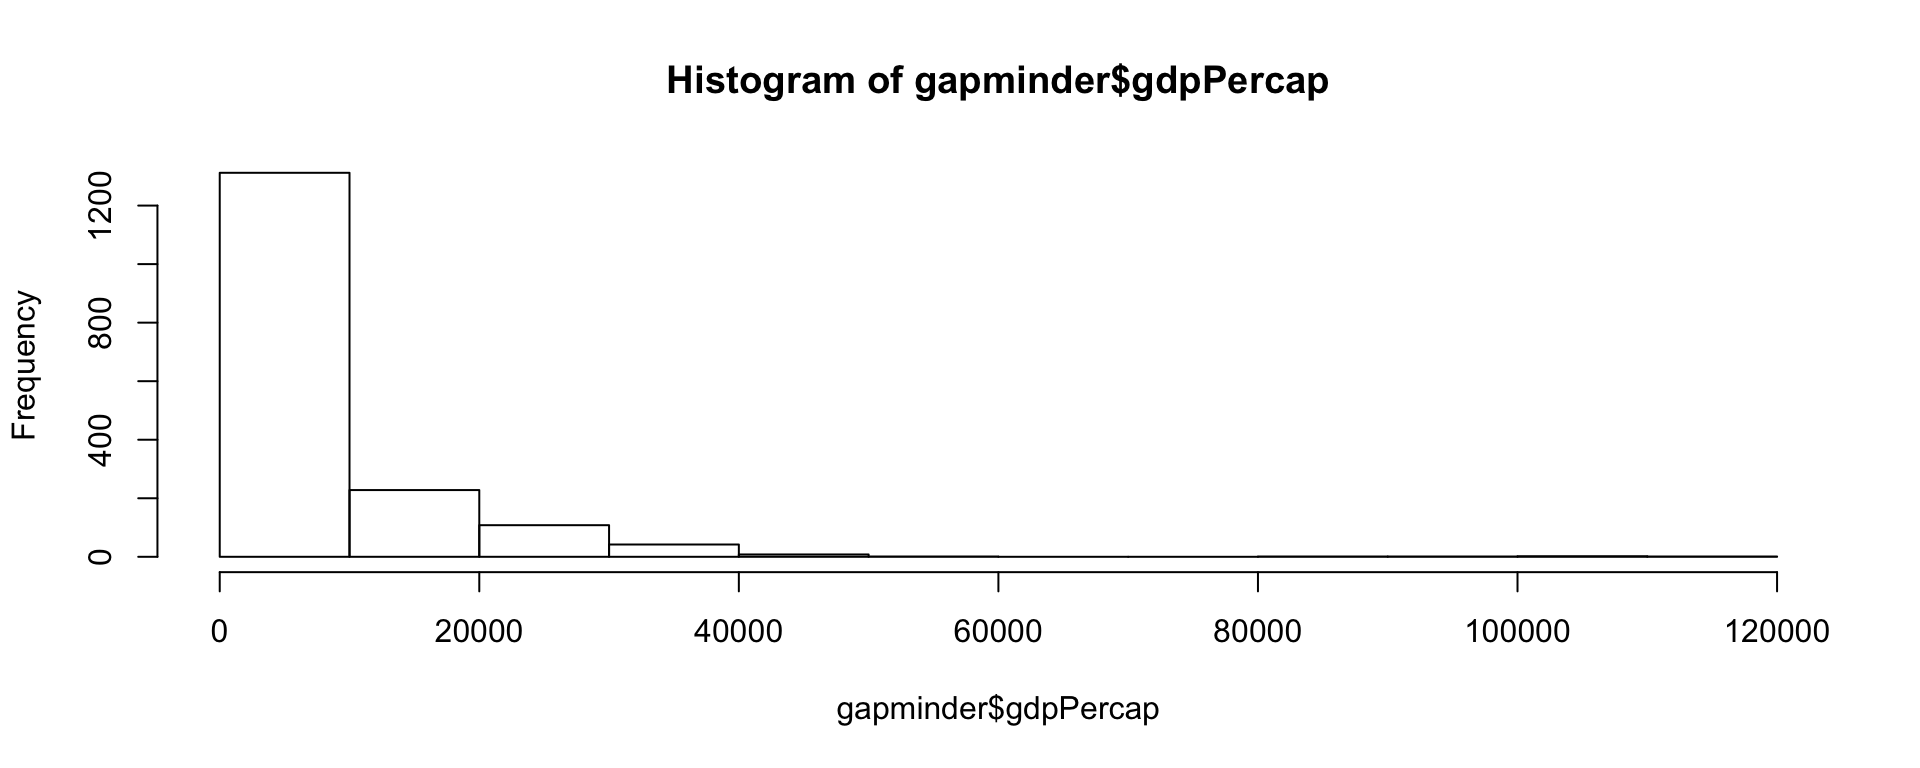
\includegraphics{R4EH_book_files/figure-latex/unnamed-chunk-23-1.pdf}

\subsection{Boxplot}\label{boxplot}

\begin{itemize}
\tightlist
\item
  Boxplots are similar syntax
\end{itemize}

\begin{Shaded}
\begin{Highlighting}[]
\KeywordTok{boxplot}\NormalTok{(gapminder}\OperatorTok{$}\NormalTok{gdpPercap)}
\end{Highlighting}
\end{Shaded}

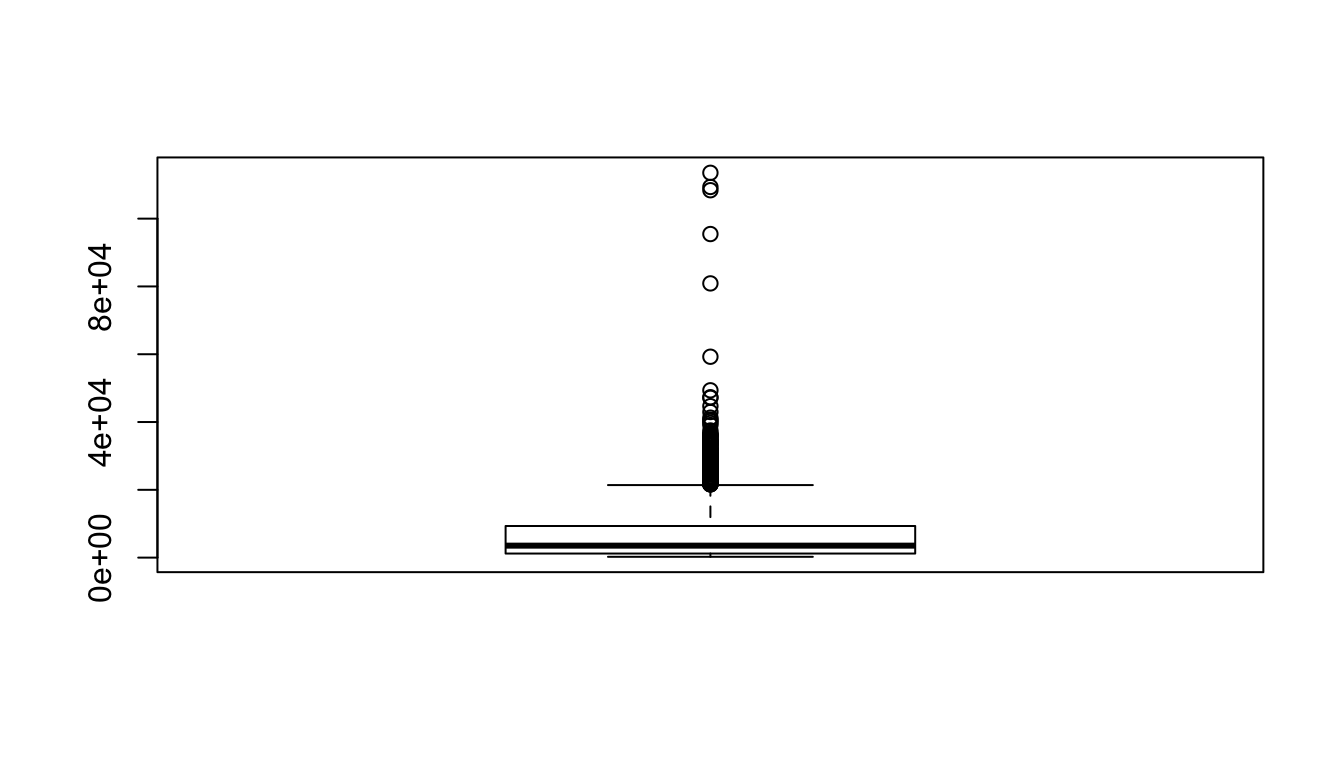
\includegraphics{R4EH_book_files/figure-latex/unnamed-chunk-24-1.pdf}

\begin{itemize}
\tightlist
\item
  If we want a boxplot for each category, use
  \texttt{variable.name\textasciitilde{}category.variable.name} to tell
  \texttt{R} to plot a boxplot \textbf{by} category
\end{itemize}

\begin{Shaded}
\begin{Highlighting}[]
\KeywordTok{boxplot}\NormalTok{(gdpPercap}\OperatorTok{~}\NormalTok{continent,}\DataTypeTok{data=}\NormalTok{gapminder)}
\end{Highlighting}
\end{Shaded}

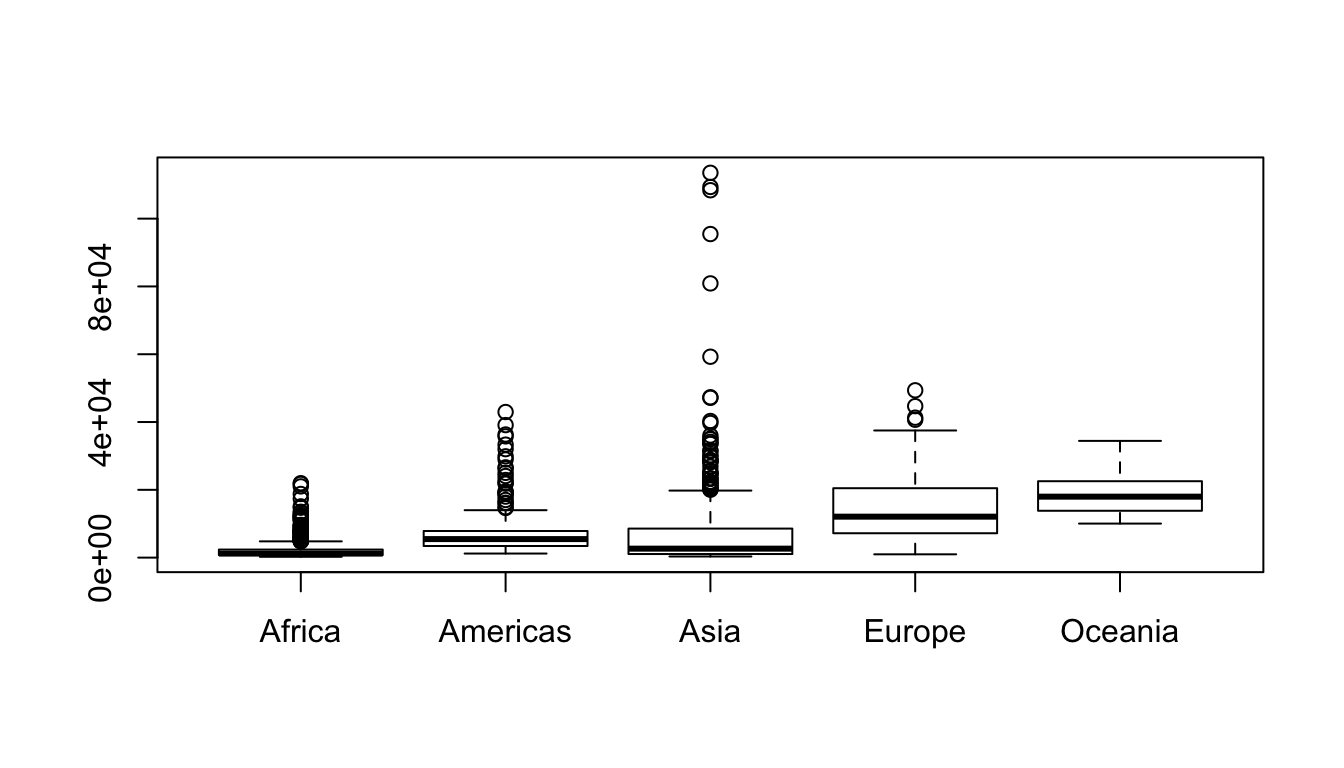
\includegraphics{R4EH_book_files/figure-latex/unnamed-chunk-25-1.pdf}

\subsection{Scatterplot}\label{scatterplot}

\begin{itemize}
\tightlist
\item
  Scatterplot syntax for plotting is similar to \texttt{hist()} and
  \texttt{boxplot()}: \texttt{plot(df\$x,df\$y)}
\end{itemize}

\begin{Shaded}
\begin{Highlighting}[]
\KeywordTok{plot}\NormalTok{(gapminder}\OperatorTok{$}\NormalTok{gdpPercap, gapminder}\OperatorTok{$}\NormalTok{lifeExp)}
\end{Highlighting}
\end{Shaded}

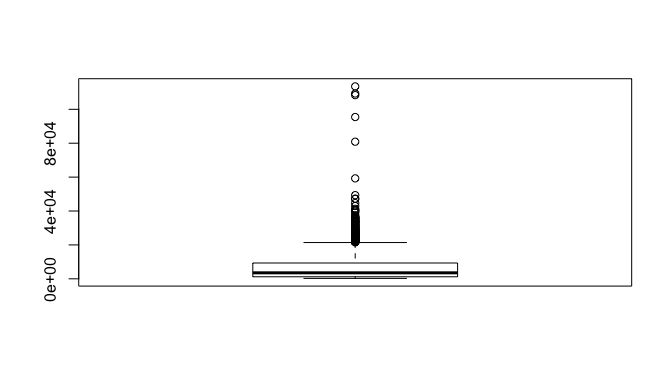
\includegraphics{R4EH_book_files/figure-latex/unnamed-chunk-26-1.pdf}

\section{\texorpdfstring{With
\texttt{ggplot2}}{With ggplot2}}\label{with-ggplot2}

`\texttt{ggplot2} is one of the premier packages at the center of the
\texttt{tidyverse}. It is very powerful and creates beautiful data
visualizations, but has a steeper learning curve at first. All of those
``cool graphics'' you see in media outlets such as the
\href{https://archive.nytimes.com/www.nytimes.com/interactive/sports/football/2013-fantasy-football-tier-charts-QB.html}{New
York Times},
\href{https://fivethirtyeight.com/features/fastest-airlines-fastest-airports/}{fivethirtyeight},
Vox, the Economist, etc use something are based off of \texttt{ggplot2}.
The \texttt{gg} stands for a ``grammar of graphics''

\subsection{Two Ways to Plot}\label{two-ways-to-plot}

\begin{enumerate}
\def\labelenumi{\arabic{enumi}.}
\tightlist
\item
  Just the single \texttt{ggplot} command

  \begin{itemize}
  \tightlist
  \item
    Will view plot right after producing it
  \item
    Does not save as an object
  \item
    Need to rerun or copy/paste full command producing plot in order to
    modify or view it again
  \item
    Can still put it in a document
  \end{itemize}
\end{enumerate}

\begin{Shaded}
\begin{Highlighting}[]
\KeywordTok{ggplot}\NormalTok{(...) }\CommentTok{# make and view plot}
\KeywordTok{ggplot}\NormalTok{(some.options) }\CommentTok{# remake plot with new options and view plot}
\end{Highlighting}
\end{Shaded}

\subsection{Two Ways to Plot II}\label{two-ways-to-plot-ii}

\begin{enumerate}
\def\labelenumi{\arabic{enumi}.}
\setcounter{enumi}{1}
\tightlist
\item
  Create an object (as usual in \texttt{R})

  \begin{itemize}
  \tightlist
  \item
    This allows you to save the plot for later (re)use
  \item
    Also allows you to modify it
  \item
    Any time you want to view display it (i.e.~for putting it in a
    document), just call up the plot by name
  \end{itemize}
\end{enumerate}

\begin{Shaded}
\begin{Highlighting}[]
\NormalTok{plot.name<-}\KeywordTok{ggplot}\NormalTok{(...) }\CommentTok{# make plot}
\NormalTok{plot.name<-plot.name}\OperatorTok{+}\NormalTok{some.options }\CommentTok{# add new options to existing plot}
\NormalTok{plot.name }\CommentTok{# view plot }
\end{Highlighting}
\end{Shaded}

\begin{Shaded}
\begin{Highlighting}[]
\NormalTok{plot.name<-}\KeywordTok{ggplot}\NormalTok{(}\DataTypeTok{data=}\NormalTok{mydf, }\DataTypeTok{mapping=}\KeywordTok{aes}\NormalTok{(}\DataTypeTok{x=}\NormalTok{xvar,}\DataTypeTok{y=}\NormalTok{yvar))}\OperatorTok{+}
\StringTok{  }\KeywordTok{geom_something}\NormalTok{(options)}\OperatorTok{+}
\StringTok{  }\NormalTok{moreoptions...}
\end{Highlighting}
\end{Shaded}

\begin{itemize}
\tightlist
\item
  \texttt{gg} ``grammar of graphics'' implies any graphic can be built
  from the same components/layers:

  \begin{enumerate}
  \def\labelenumi{\arabic{enumi}.}
  \tightlist
  \item
    \textbf{Data}: base-layer describes the data used

    \begin{itemize}
    \tightlist
    \item
      \texttt{mydf} is the dataframe containing \texttt{xvar} and
      \texttt{yvar}
    \item
      \texttt{aes()} ``aesthetics'' identifies \texttt{xvar} (and if
      applicable \texttt{yvar}) from data to be ``mapped'' to a visual
      mark
    \end{itemize}
  \item
    \textbf{Geoms}: visual marks that represent data observations or
    models, common examples:

    \begin{itemize}
    \tightlist
    \item
      e.g. \texttt{geom\_point}, \texttt{geom\_line},
      \texttt{geom\_bar}, \texttt{geom\_histogram},
      \texttt{geom\_density}, \texttt{geom\_boxplot}
    \end{itemize}
  \item
    \textbf{Coordinates}: Cartesian coordinates are default

    \begin{itemize}
    \tightlist
    \item
      change scales, axes, labels, etc; advanced options like maps
    \end{itemize}
  \end{enumerate}
\item
  Most important idea to master is \texttt{aes()} \textbf{aesthetics}
  that map data to visual markings
\item
  Aesthetics come in many forms and many options, depending on the
  context of the data

  \begin{itemize}
  \tightlist
  \item
    Must identify position (e.g.~what is \texttt{x} and \texttt{y})
  \item
    Determine the marking with various \texttt{geoms} (points, bars,
    lines, boxes, etc)
  \item
    Can pass additional options into \texttt{geom} (color, size, shape,
    etc)

    \begin{itemize}
    \tightlist
    \item
      Particularly important if we want color, size, or shape to depend
      on a particular variable in dataset
    \end{itemize}
  \end{itemize}
\end{itemize}

\begin{figure}
\centering
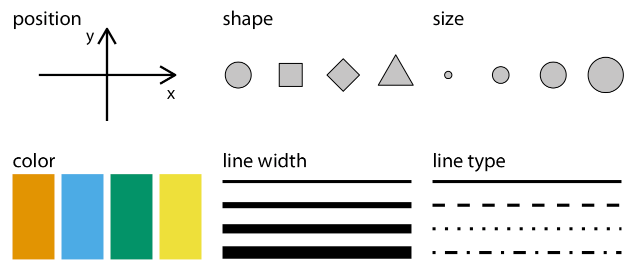
\includegraphics[height=1.50000in]{images/ggplotaes.png}
\caption{}
\end{figure}

For our example, we'll use the
\href{https://ggplot2.tidyverse.org/reference/mpg.html}{mpg dataset}
loaded with the \texttt{ggplot2} package

\begin{Shaded}
\begin{Highlighting}[]
\KeywordTok{library}\NormalTok{(}\StringTok{"ggplot2"}\NormalTok{) }\CommentTok{#load ggplot2}
\NormalTok{mpg }\CommentTok{#look at dataset}
\end{Highlighting}
\end{Shaded}

\begin{verbatim}
## # A tibble: 234 x 11
##    manufacturer model    displ  year   cyl trans   drv     cty   hwy fl   
##    <chr>        <chr>    <dbl> <int> <int> <chr>   <chr> <int> <int> <chr>
##  1 audi         a4         1.8  1999     4 auto(l~ f        18    29 p    
##  2 audi         a4         1.8  1999     4 manual~ f        21    29 p    
##  3 audi         a4         2    2008     4 manual~ f        20    31 p    
##  4 audi         a4         2    2008     4 auto(a~ f        21    30 p    
##  5 audi         a4         2.8  1999     6 auto(l~ f        16    26 p    
##  6 audi         a4         2.8  1999     6 manual~ f        18    26 p    
##  7 audi         a4         3.1  2008     6 auto(a~ f        18    27 p    
##  8 audi         a4 quat~   1.8  1999     4 manual~ 4        18    26 p    
##  9 audi         a4 quat~   1.8  1999     4 auto(l~ 4        16    25 p    
## 10 audi         a4 quat~   2    2008     4 manual~ 4        20    28 p    
## # ... with 224 more rows, and 1 more variable: class <chr>
\end{verbatim}

\begin{itemize}
\tightlist
\item
  Start with the \textbf{base layer}: establish the data source, define
  \(x\) variable
\end{itemize}

\begin{Shaded}
\begin{Highlighting}[]
\NormalTok{mpg.h<-}\KeywordTok{ggplot}\NormalTok{(}\DataTypeTok{data=}\NormalTok{mpg,}\DataTypeTok{mapping=}\KeywordTok{aes}\NormalTok{(}\DataTypeTok{x=}\NormalTok{hwy))}
\NormalTok{mpg.h}
\end{Highlighting}
\end{Shaded}

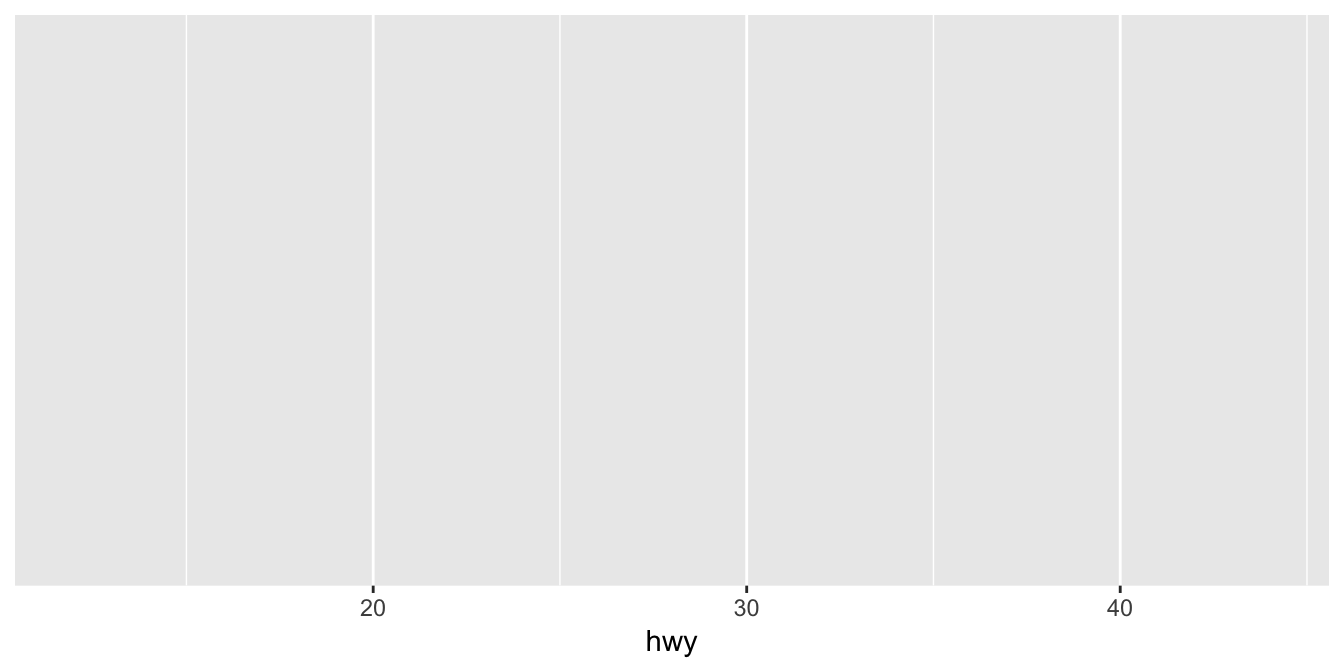
\includegraphics{R4EH_book_files/figure-latex/unnamed-chunk-31-1.pdf}

\begin{itemize}
\tightlist
\item
  Add a histogram \texttt{geom\_} layer of \texttt{hwy}
\end{itemize}

\begin{Shaded}
\begin{Highlighting}[]
\NormalTok{mpg.h1<-mpg.h}\OperatorTok{+}\KeywordTok{geom_histogram}\NormalTok{()}
\NormalTok{mpg.h1}
\end{Highlighting}
\end{Shaded}

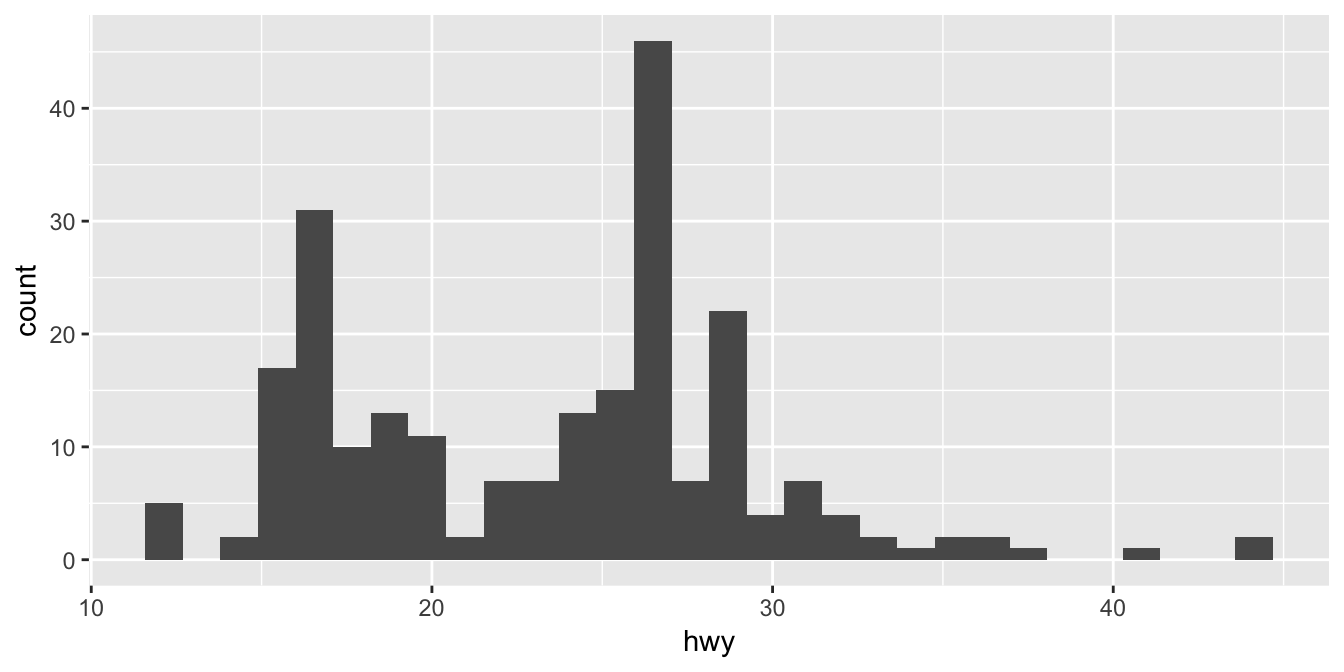
\includegraphics{R4EH_book_files/figure-latex/unnamed-chunk-32-1.pdf}

\begin{itemize}
\tightlist
\item
  Customize the histogram \texttt{geom\_} layer (\# of bins, color, etc)
\end{itemize}

\begin{Shaded}
\begin{Highlighting}[]
\NormalTok{mpg.h2<-mpg.h}\OperatorTok{+}\KeywordTok{geom_histogram}\NormalTok{(}\DataTypeTok{bins=}\DecValTok{20}\NormalTok{, }\DataTypeTok{color=}\StringTok{"black"}\NormalTok{,}\DataTypeTok{fill=}\StringTok{"indianred"}\NormalTok{)}
\NormalTok{mpg.h2}
\end{Highlighting}
\end{Shaded}

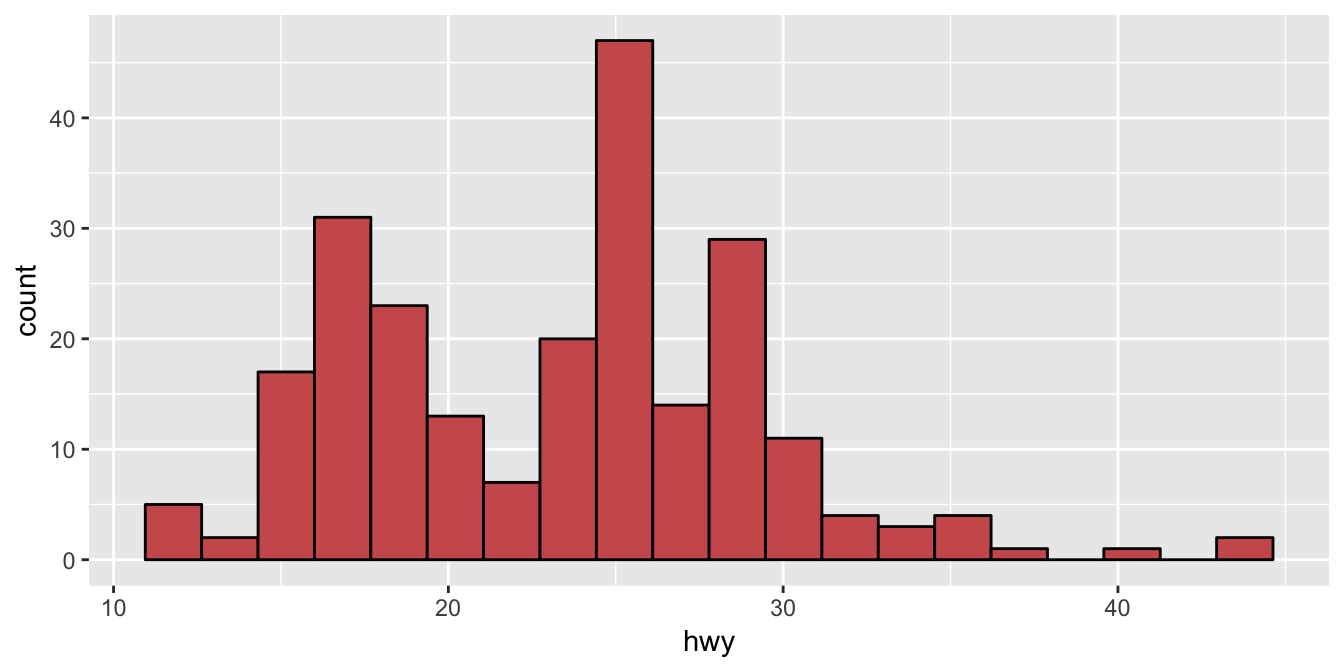
\includegraphics{R4EH_book_files/figure-latex/unnamed-chunk-33-1.pdf}

\begin{itemize}
\item
  Adding additional \texttt{geom\_} layers
\item
  Add a vertical line for the mean with another \texttt{geom} called
  \texttt{vline}
\end{itemize}

\begin{Shaded}
\begin{Highlighting}[]
\NormalTok{mpg.h2<-mpg.h2}\OperatorTok{+}
\StringTok{  }\KeywordTok{geom_vline}\NormalTok{(}\DataTypeTok{xintercept=}\KeywordTok{mean}\NormalTok{(mpg}\OperatorTok{$}\NormalTok{hwy),}\DataTypeTok{linetype=}\StringTok{"dotted"}\NormalTok{,}\DataTypeTok{color=}\StringTok{"blue"}\NormalTok{,}\DataTypeTok{size=}\DecValTok{1}\NormalTok{)}
\NormalTok{mpg.h2}
\end{Highlighting}
\end{Shaded}

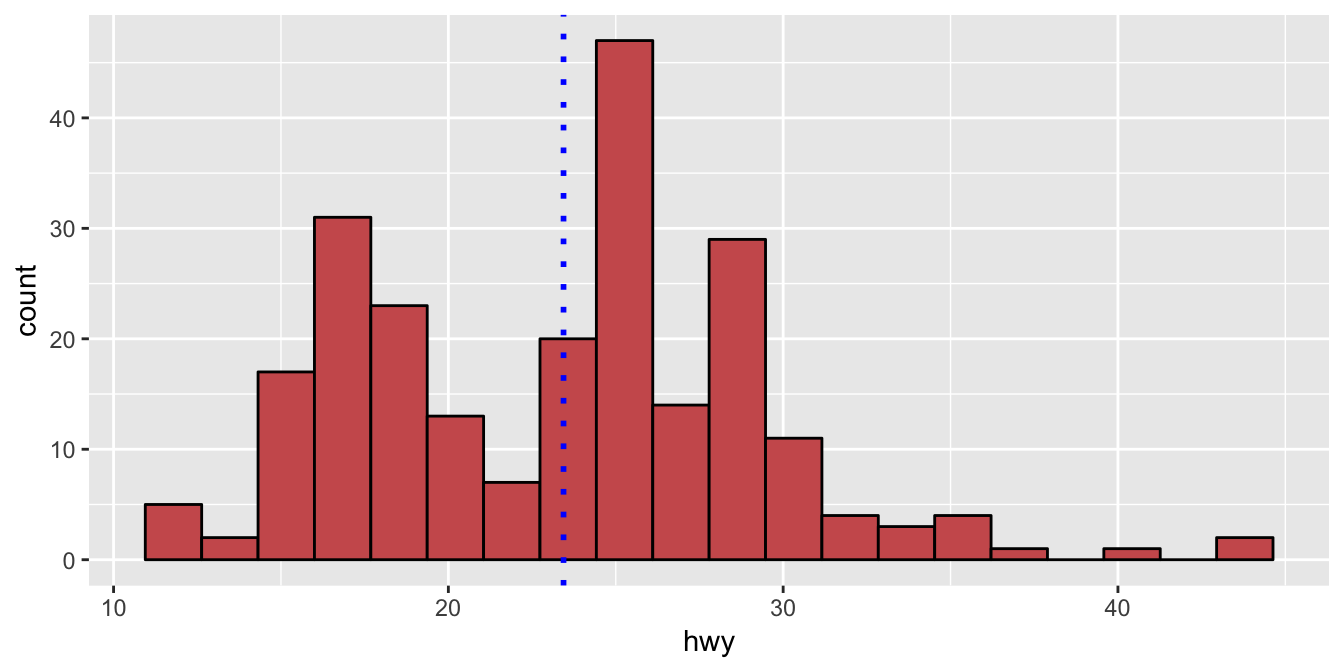
\includegraphics{R4EH_book_files/figure-latex/unnamed-chunk-34-1.pdf}

\begin{itemize}
\item
  Editing Coordinates (Axes)
\item
  Change the labels on the axes with \texttt{xlab()} and \texttt{ylab()}
\end{itemize}

\begin{Shaded}
\begin{Highlighting}[]
\NormalTok{mpg.h2<-mpg.h2}\OperatorTok{+}\KeywordTok{xlab}\NormalTok{(}\StringTok{"Miles Per Gallon (on Highway)"}\NormalTok{)}\OperatorTok{+}\KeywordTok{ylab}\NormalTok{(}\StringTok{"Number of Cars"}\NormalTok{)}
\NormalTok{mpg.h2}
\end{Highlighting}
\end{Shaded}

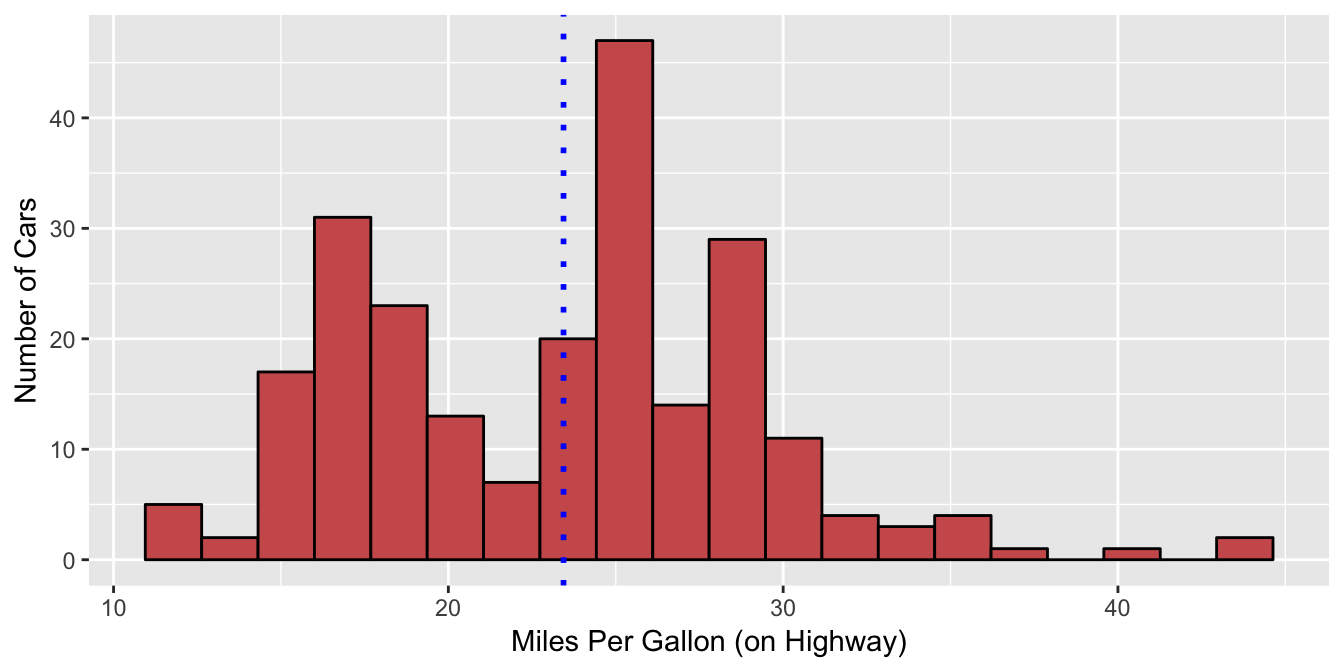
\includegraphics{R4EH_book_files/figure-latex/unnamed-chunk-35-1.pdf}

Other Geoms

\begin{itemize}
\tightlist
\item
  How about a \textbf{density plot}: use \texttt{geom\_density()}
  instead of \texttt{geom\_histogram()}
\end{itemize}

\begin{Shaded}
\begin{Highlighting}[]
\NormalTok{mpg.d<-}\KeywordTok{ggplot}\NormalTok{(}\DataTypeTok{data=}\NormalTok{mpg,}\KeywordTok{aes}\NormalTok{(}\DataTypeTok{x=}\NormalTok{hwy))}\OperatorTok{+}
\StringTok{  }\KeywordTok{geom_density}\NormalTok{(}\DataTypeTok{fill=}\StringTok{"indianred"}\NormalTok{)}
\NormalTok{mpg.d}
\end{Highlighting}
\end{Shaded}

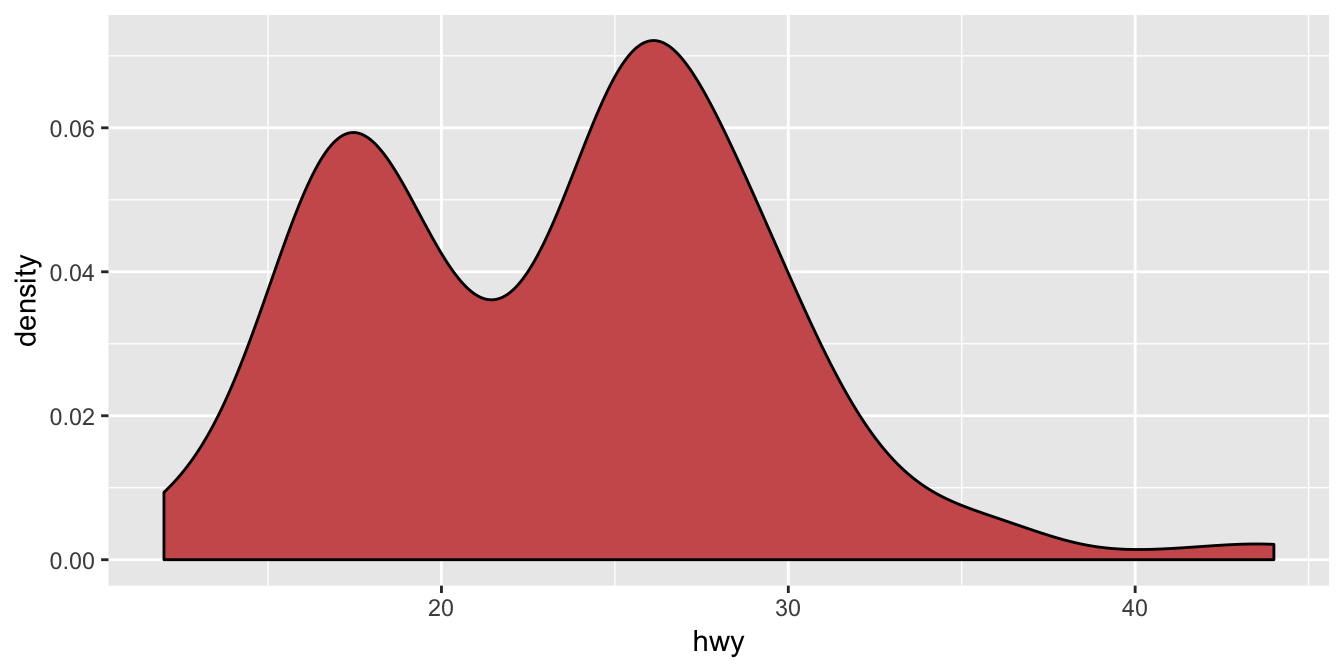
\includegraphics{R4EH_book_files/figure-latex/unnamed-chunk-36-1.pdf}

\begin{itemize}
\tightlist
\item
  Let's make a separate density plot for each \texttt{class}, set
  \texttt{aes} to \texttt{fill} by \texttt{class}
\end{itemize}

\begin{Shaded}
\begin{Highlighting}[]
\NormalTok{mpg.d<-}\KeywordTok{ggplot}\NormalTok{(}\DataTypeTok{data=}\NormalTok{mpg,}\KeywordTok{aes}\NormalTok{(}\DataTypeTok{x=}\NormalTok{hwy,}\DataTypeTok{fill=}\NormalTok{class))}\OperatorTok{+}
\StringTok{  }\KeywordTok{geom_density}\NormalTok{(}\DataTypeTok{alpha=}\FloatTok{0.5}\NormalTok{) }\CommentTok{# alpha adds transparency}
\NormalTok{mpg.d}
\end{Highlighting}
\end{Shaded}

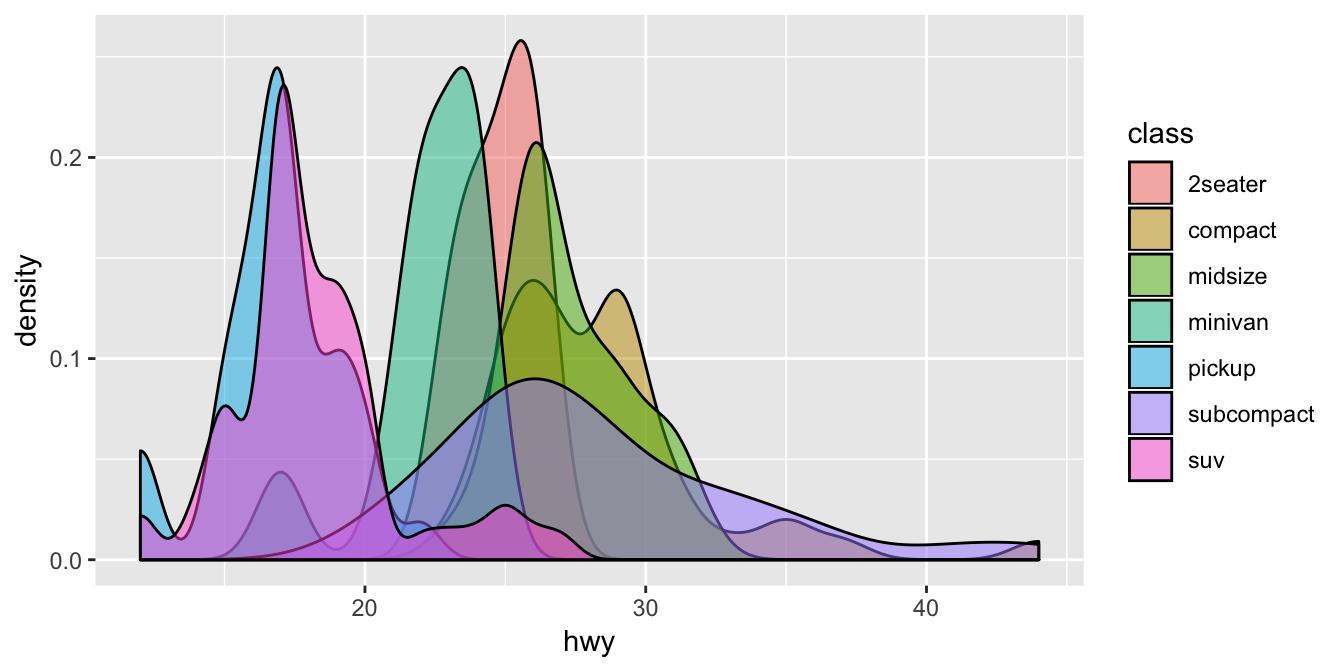
\includegraphics{R4EH_book_files/figure-latex/unnamed-chunk-37-1.pdf}

\begin{itemize}
\tightlist
\item
  Instead of a density plot, a \texttt{boxplot} by \texttt{class} (note
  now \texttt{x} is \texttt{class} and \texttt{y} is \texttt{hwy}):
\end{itemize}

\begin{Shaded}
\begin{Highlighting}[]
\NormalTok{mpg.b<-}\KeywordTok{ggplot}\NormalTok{(}\DataTypeTok{data=}\NormalTok{mpg,}\KeywordTok{aes}\NormalTok{(}\DataTypeTok{x=}\NormalTok{class,}\DataTypeTok{y=}\NormalTok{hwy,}\DataTypeTok{fill=}\NormalTok{class))}\OperatorTok{+}
\StringTok{  }\KeywordTok{geom_boxplot}\NormalTok{()}
\NormalTok{mpg.b}
\end{Highlighting}
\end{Shaded}

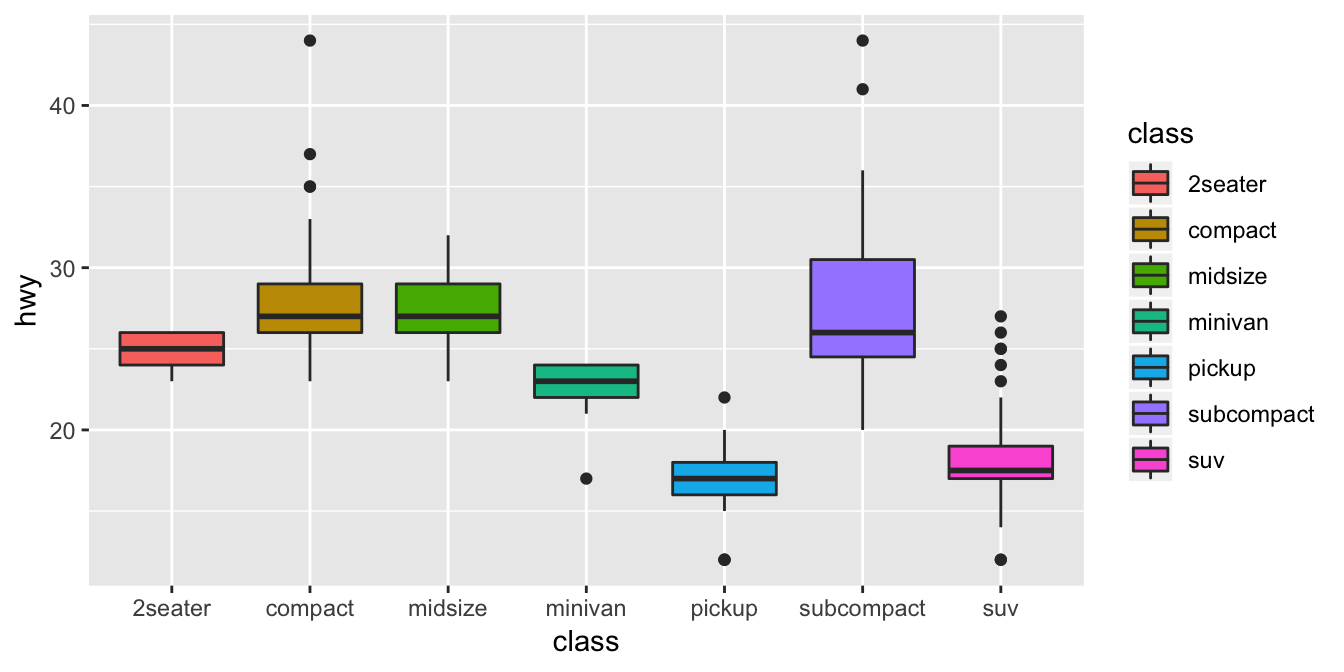
\includegraphics{R4EH_book_files/figure-latex/unnamed-chunk-38-1.pdf}

\begin{itemize}
\tightlist
\item
  Start with the base layer: establish data source, define \(x\) and
  \(y\) variables
\end{itemize}

\begin{Shaded}
\begin{Highlighting}[]
\NormalTok{mpg.p<-}\KeywordTok{ggplot}\NormalTok{(}\DataTypeTok{data=}\NormalTok{mpg,}\KeywordTok{aes}\NormalTok{(}\DataTypeTok{x=}\NormalTok{displ, }\DataTypeTok{y=}\NormalTok{hwy)) }\CommentTok{#use mtcars df, let x=displ, y=hwy}

\NormalTok{mpg.p}
\end{Highlighting}
\end{Shaded}

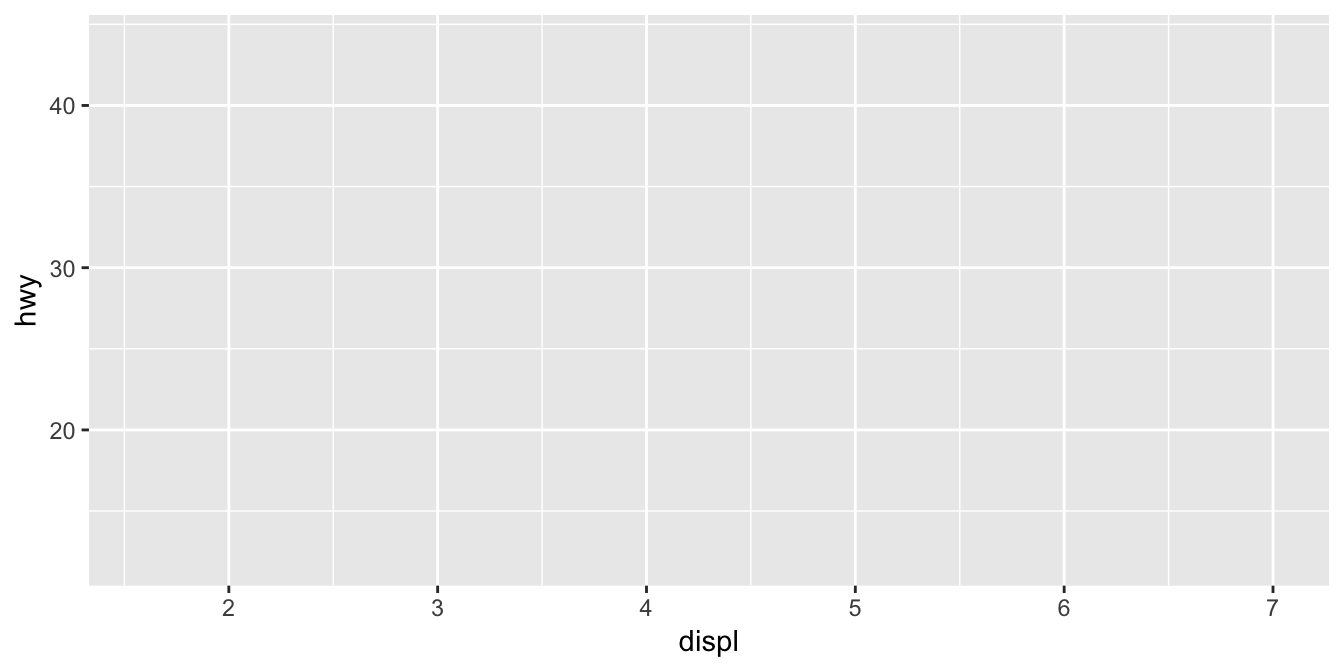
\includegraphics{R4EH_book_files/figure-latex/unnamed-chunk-39-1.pdf}

\begin{Shaded}
\begin{Highlighting}[]
\NormalTok{mpg.p<-mpg.p}\OperatorTok{+}\KeywordTok{geom_point}\NormalTok{() }\CommentTok{# specify observations as points on graph}

\NormalTok{mpg.p}
\end{Highlighting}
\end{Shaded}

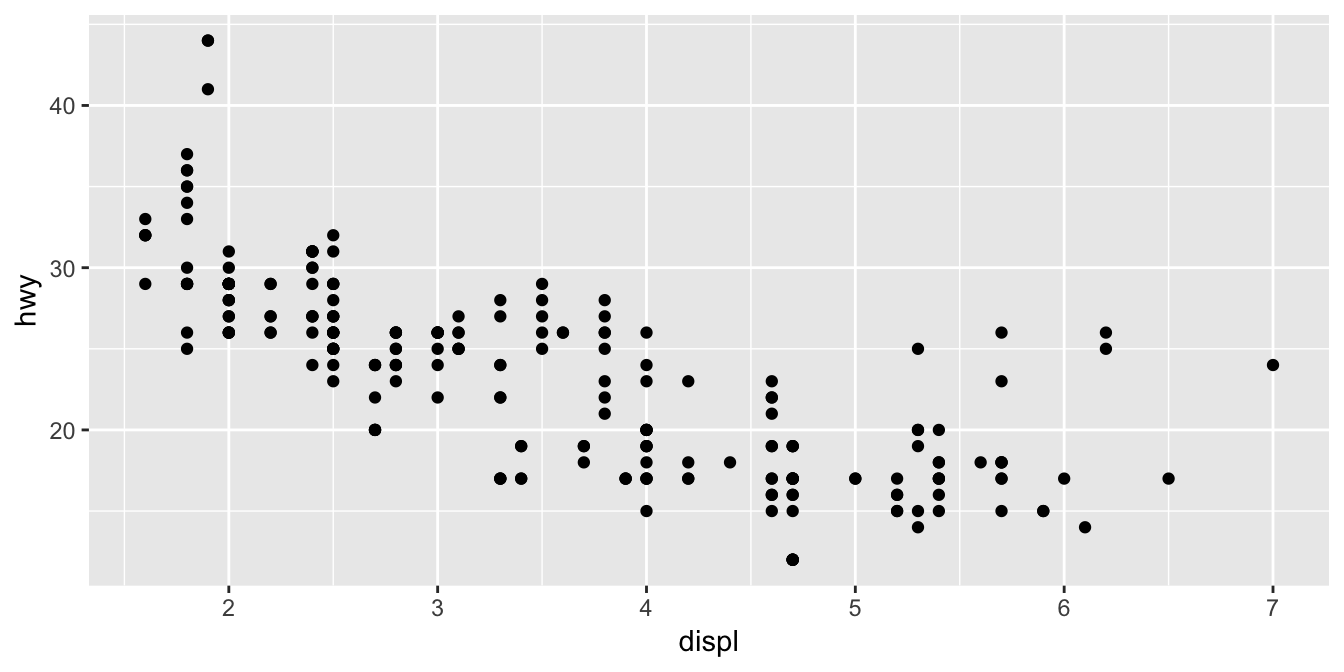
\includegraphics{R4EH_book_files/figure-latex/unnamed-chunk-40-1.pdf}

\begin{Shaded}
\begin{Highlighting}[]
\NormalTok{mpg.p<-mpg.p}\OperatorTok{+}\KeywordTok{geom_point}\NormalTok{(}\KeywordTok{aes}\NormalTok{(}\DataTypeTok{color=}\NormalTok{manufacturer)) }\CommentTok{# color data points by manuf.}

\NormalTok{mpg.p}
\end{Highlighting}
\end{Shaded}

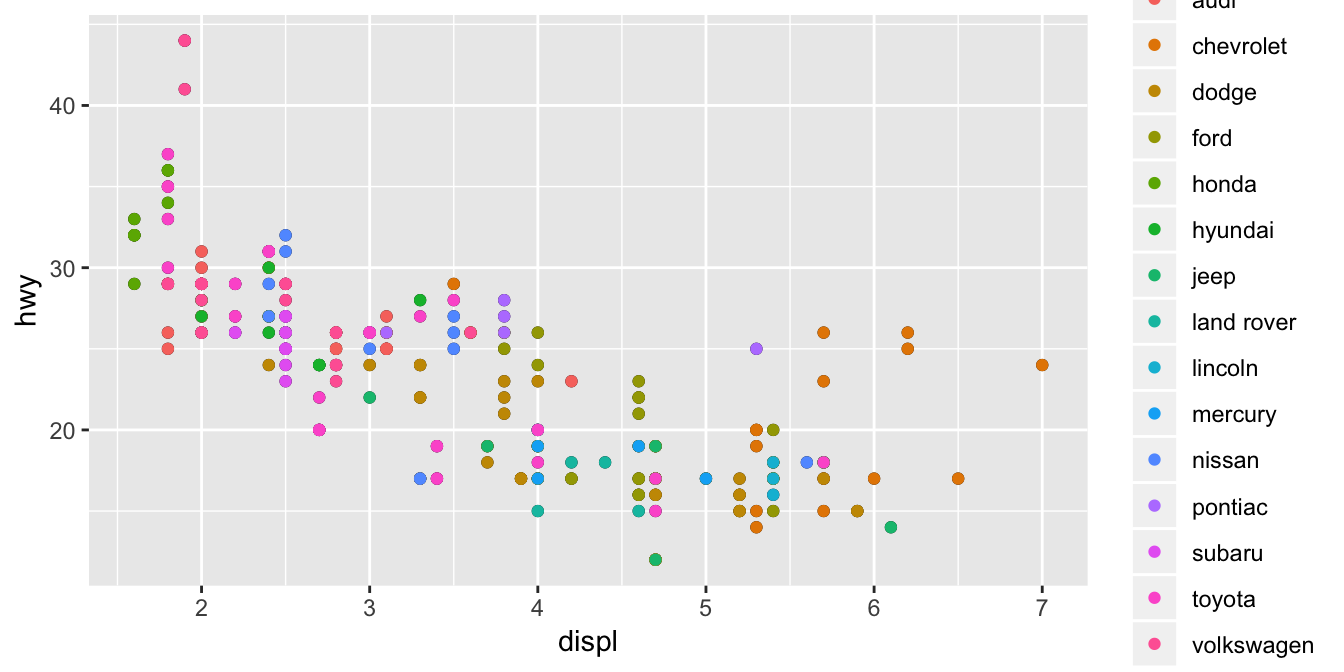
\includegraphics{R4EH_book_files/figure-latex/unnamed-chunk-41-1.pdf}

\begin{Shaded}
\begin{Highlighting}[]
\NormalTok{mpg.p<-mpg.p}\OperatorTok{+}\KeywordTok{geom_smooth}\NormalTok{(}\DataTypeTok{method=}\StringTok{"lm"}\NormalTok{, }\DataTypeTok{color=}\StringTok{"black"}\NormalTok{) }\CommentTok{# add a black OLS line }

\NormalTok{mpg.p}
\end{Highlighting}
\end{Shaded}

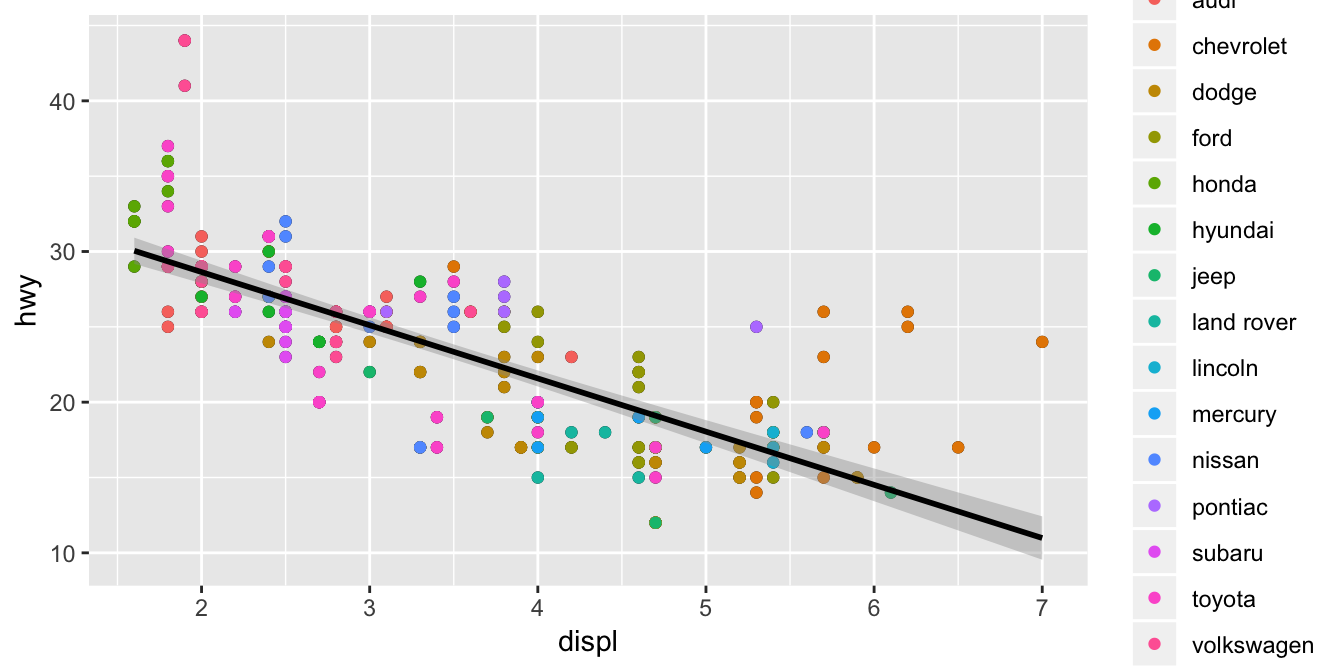
\includegraphics{R4EH_book_files/figure-latex/unnamed-chunk-42-1.pdf}

\begin{Shaded}
\begin{Highlighting}[]
\NormalTok{mpg.p<-mpg.p}\OperatorTok{+}\KeywordTok{xlab}\NormalTok{(}\StringTok{"Engine Displacement (Liters)"}\NormalTok{)}\OperatorTok{+}
\StringTok{  }\KeywordTok{ylab}\NormalTok{(}\StringTok{"Miles Per Gallon on Highway"}\NormalTok{)}
\NormalTok{mpg.p}
\end{Highlighting}
\end{Shaded}

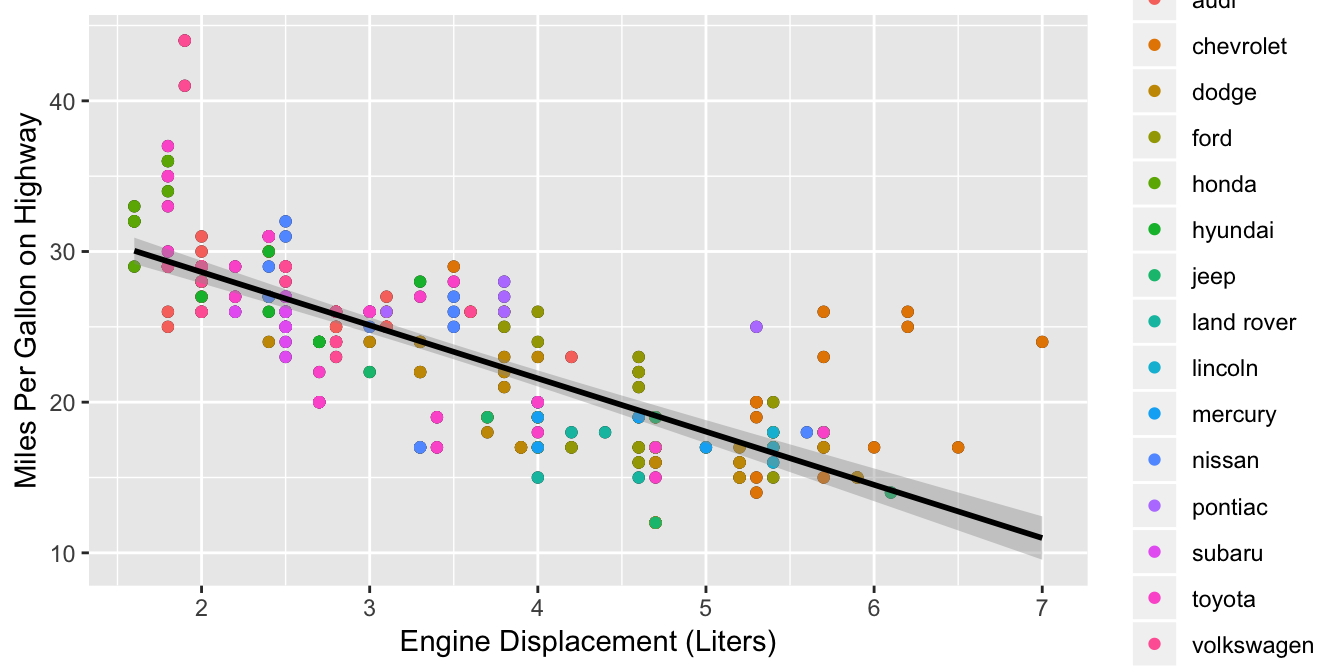
\includegraphics{R4EH_book_files/figure-latex/unnamed-chunk-43-1.pdf}

\begin{itemize}
\tightlist
\item
  Let's have some fun changing the theme
\end{itemize}

\begin{Shaded}
\begin{Highlighting}[]
\KeywordTok{library}\NormalTok{(}\StringTok{"ggthemes"}\NormalTok{) }\CommentTok{# need ggthemes package (install if first use)}
\NormalTok{mpg.p<-mpg.p}\OperatorTok{+}\KeywordTok{theme_economist_white}\NormalTok{() }\CommentTok{#make it look like The Economist magazine}
\NormalTok{mpg.p}
\end{Highlighting}
\end{Shaded}

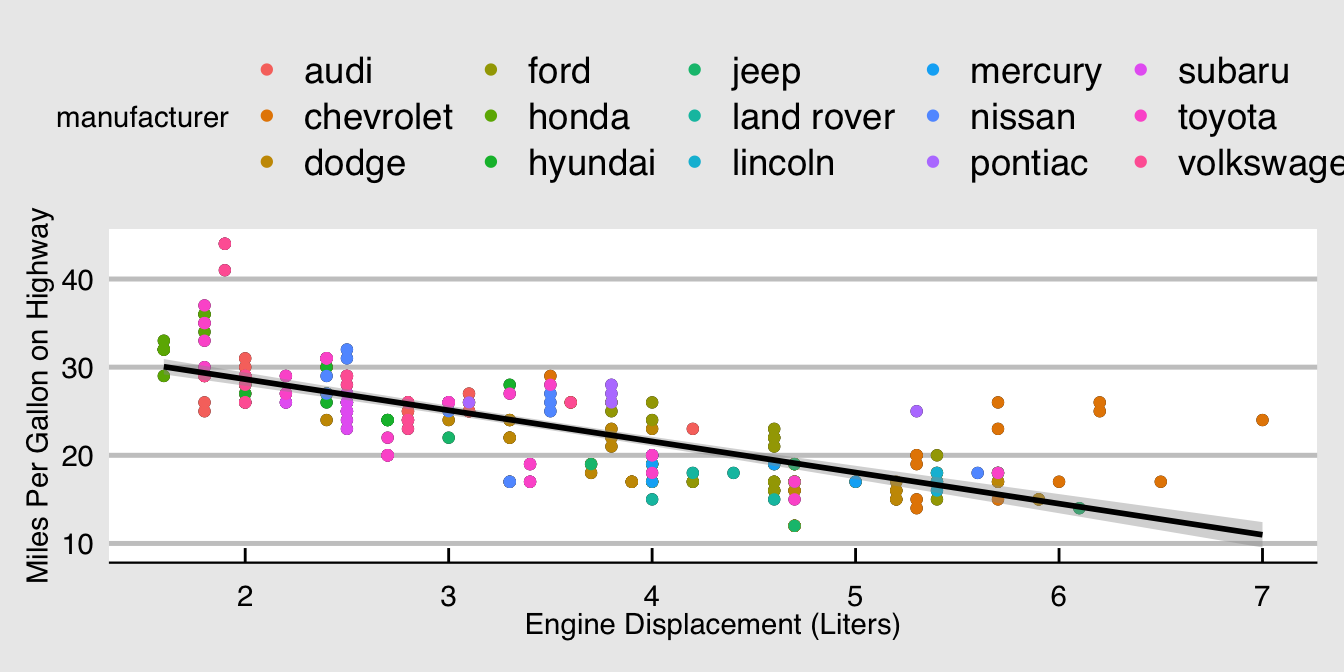
\includegraphics{R4EH_book_files/figure-latex/unnamed-chunk-44-1.pdf}

\begin{Shaded}
\begin{Highlighting}[]
\NormalTok{mpg.p<-mpg.p}\OperatorTok{+}\KeywordTok{theme_fivethirtyeight}\NormalTok{() }\CommentTok{#make it look like fivethirtyeight}
\NormalTok{mpg.p}
\end{Highlighting}
\end{Shaded}

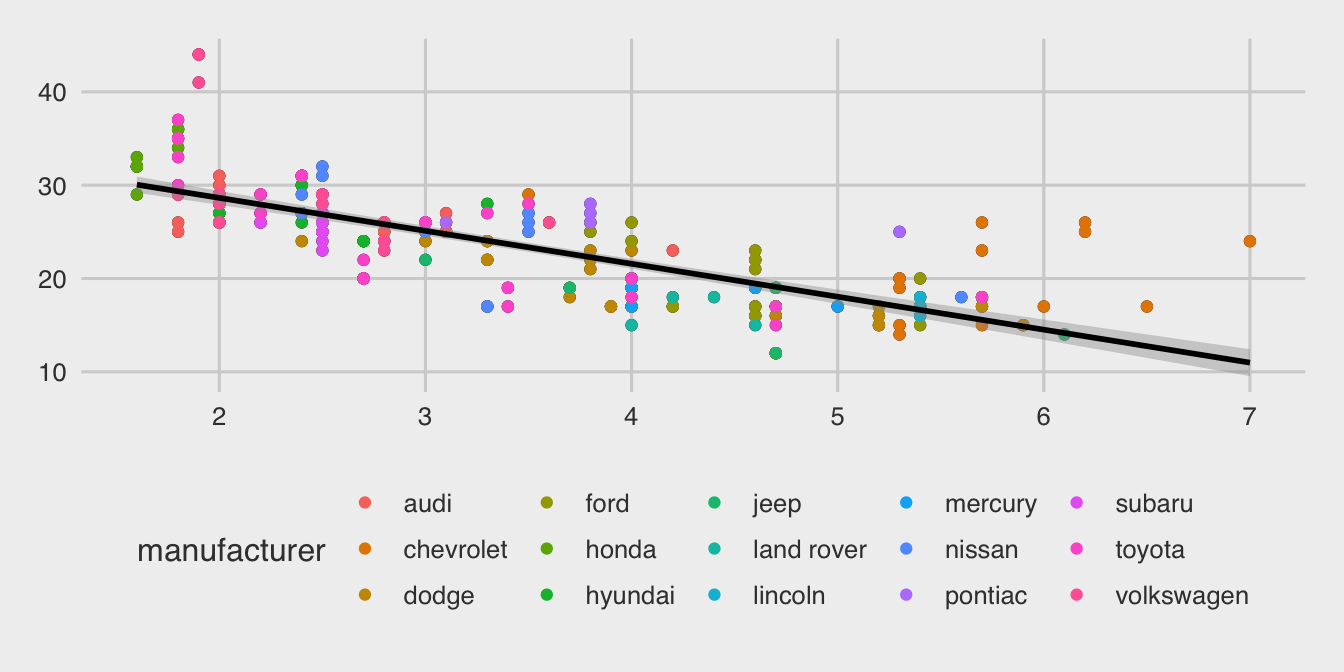
\includegraphics{R4EH_book_files/figure-latex/unnamed-chunk-45-1.pdf}

\begin{Shaded}
\begin{Highlighting}[]
\CommentTok{# make columns of separate 'facet' figures for each class of car}
\NormalTok{mpg.p<-mpg.p}\OperatorTok{+}\KeywordTok{facet_grid}\NormalTok{(}\DataTypeTok{cols =} \KeywordTok{vars}\NormalTok{(class)) }\CommentTok{# make 'columns' by variable 'class'}
\NormalTok{mpg.p}
\end{Highlighting}
\end{Shaded}

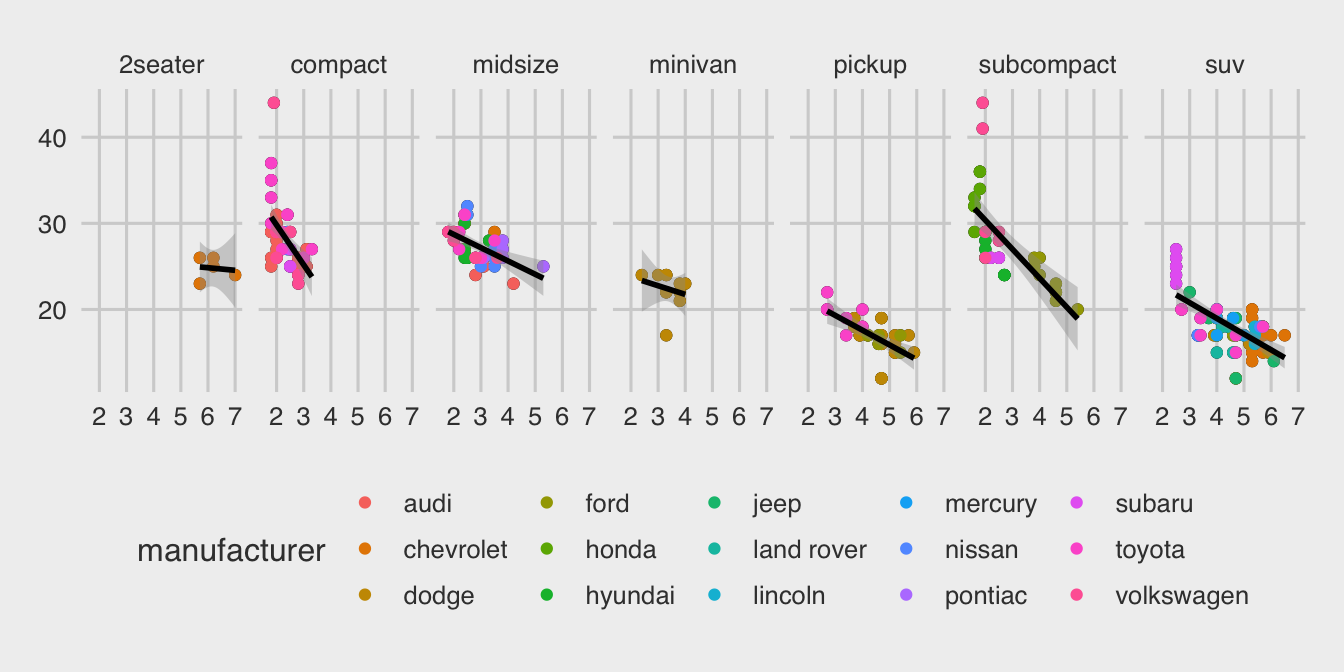
\includegraphics{R4EH_book_files/figure-latex/unnamed-chunk-46-1.pdf}

\begin{Shaded}
\begin{Highlighting}[]
\KeywordTok{ggplot}\NormalTok{(}\DataTypeTok{data=}\NormalTok{mpg,}\KeywordTok{aes}\NormalTok{(}\DataTypeTok{x=}\NormalTok{displ, }\DataTypeTok{y=}\NormalTok{hwy))}\OperatorTok{+}\KeywordTok{geom_point}\NormalTok{(}\KeywordTok{aes}\NormalTok{(}\DataTypeTok{color=}\NormalTok{manufacturer))}\OperatorTok{+}
\StringTok{  }\KeywordTok{geom_smooth}\NormalTok{(}\DataTypeTok{color=}\StringTok{"black"}\NormalTok{,}\DataTypeTok{method=}\StringTok{"lm"}\NormalTok{)}\OperatorTok{+}
\StringTok{  }\KeywordTok{xlab}\NormalTok{(}\StringTok{"Engine Displacement (Liters)"}\NormalTok{)}\OperatorTok{+}\KeywordTok{ylab}\NormalTok{(}\StringTok{"Miles Per Gallon on Highway"}\NormalTok{)}\OperatorTok{+}
\StringTok{  }\KeywordTok{theme_fivethirtyeight}\NormalTok{()}\OperatorTok{+}\KeywordTok{facet_grid}\NormalTok{(}\DataTypeTok{cols =} \KeywordTok{vars}\NormalTok{(class)) }
\end{Highlighting}
\end{Shaded}

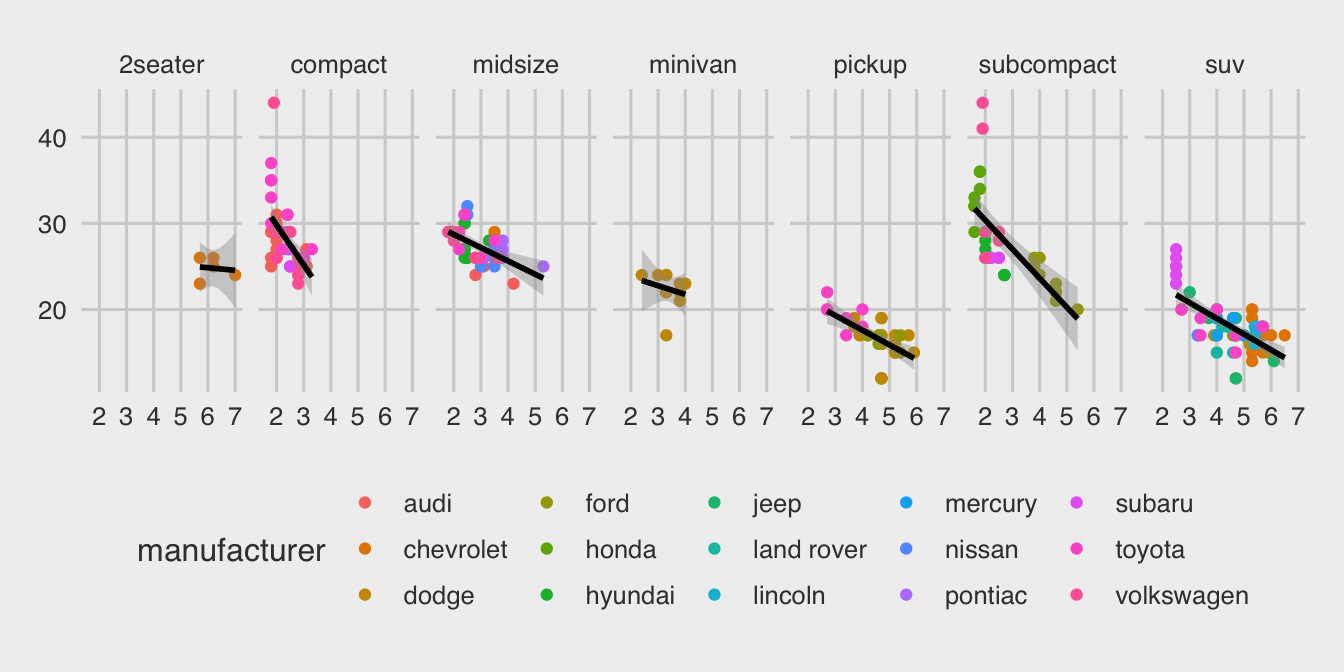
\includegraphics{R4EH_book_files/figure-latex/unnamed-chunk-47-1.pdf}

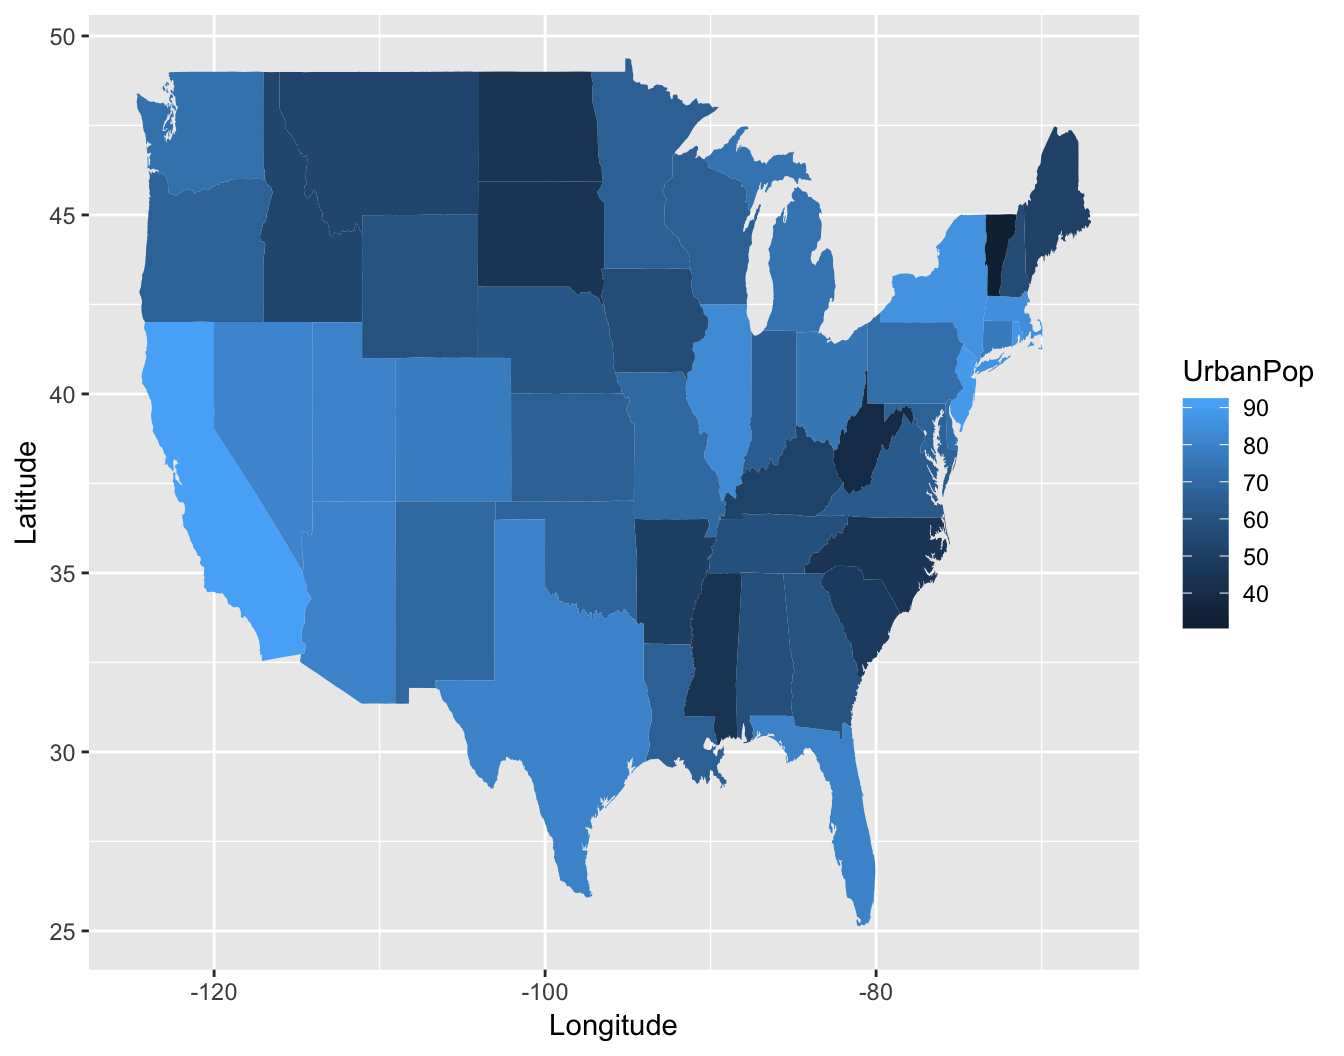
\includegraphics{R4EH_book_files/figure-latex/unnamed-chunk-48-1.pdf}

\chapter{Regression Basics}\label{regression-basics}

\section{Ordinary Least Squares (OLS)
Regression}\label{ordinary-least-squares-ols-regression}

In \texttt{R}, the Ordinary Least Squares (OLS) regression model is
simply called the \textbf{``linear model''}, abbreviated \texttt{lm}.
Regressions are run on several variables from a \texttt{data.frame} and
stored as a \texttt{lm} object that we can inspect and modify.

\begin{Shaded}
\begin{Highlighting}[]
\NormalTok{set.seed=}\DecValTok{1} \CommentTok{#makes 'random' draws reproducible }
\NormalTok{x<-}\KeywordTok{runif}\NormalTok{(}\DecValTok{500}\NormalTok{,}\DataTypeTok{min=}\DecValTok{0}\NormalTok{,}\DataTypeTok{max=}\DecValTok{10}\NormalTok{) }\CommentTok{#500 draws from uniform distr }
\NormalTok{y<-}\DecValTok{2}\OperatorTok{*}\NormalTok{x}\OperatorTok{+}\KeywordTok{rnorm}\NormalTok{(}\DecValTok{500}\NormalTok{,}\DecValTok{2}\NormalTok{,}\DecValTok{4}\NormalTok{)}
\NormalTok{my_df<-}\KeywordTok{data.frame}\NormalTok{(x,y)}

\KeywordTok{ggplot}\NormalTok{(my_df, }\KeywordTok{aes}\NormalTok{(}\DataTypeTok{x=}\NormalTok{x,}\DataTypeTok{y=}\NormalTok{y))}\OperatorTok{+}
\StringTok{        }\KeywordTok{geom_point}\NormalTok{(}\DataTypeTok{alpha=}\FloatTok{0.5}\NormalTok{)}\OperatorTok{+}
\StringTok{        }\KeywordTok{geom_smooth}\NormalTok{(}\DataTypeTok{method=}\StringTok{"lm"}\NormalTok{, }\DataTypeTok{color=}\StringTok{"green"}\NormalTok{)}\OperatorTok{+}
\StringTok{        }\KeywordTok{xlim}\NormalTok{(}\KeywordTok{c}\NormalTok{(}\DecValTok{0}\NormalTok{,}\DecValTok{10}\NormalTok{))}\OperatorTok{+}\KeywordTok{theme_light}\NormalTok{()}
\end{Highlighting}
\end{Shaded}

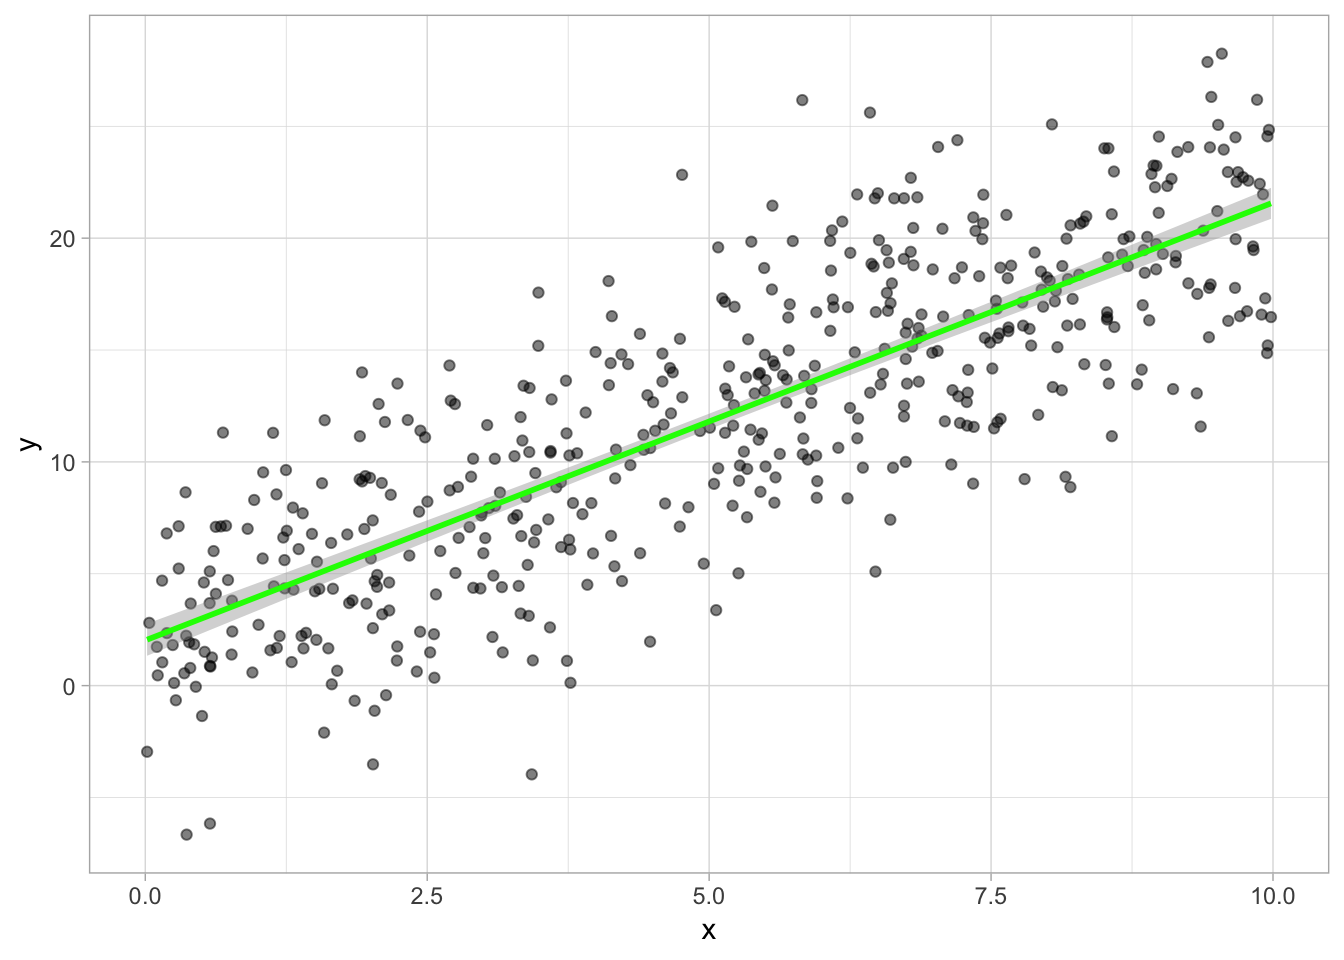
\includegraphics{R4EH_book_files/figure-latex/unnamed-chunk-50-1.pdf}

The syntax for running a regression in \texttt{R} is simple. We store
the regression as an \texttt{lm()} object (e.g.~called
``\texttt{my\_reg}'') and regress our dependent (\texttt{mydf\$y})
variable on (\texttt{\textasciitilde{}}) the independent
(\texttt{my\_df\$x}) variable.

\begin{Shaded}
\begin{Highlighting}[]
\NormalTok{my_reg<-}\KeywordTok{lm}\NormalTok{(df}\OperatorTok{$}\NormalTok{y}\OperatorTok{~}\NormalTok{df}\OperatorTok{$}\NormalTok{x)}
\end{Highlighting}
\end{Shaded}

Alternatively, we can simply use the variable \texttt{names} from
\texttt{my\_df} and then tell \texttt{R} that the variables are coming
from \texttt{my\_df}:

\begin{Shaded}
\begin{Highlighting}[]
\NormalTok{my_reg<-}\KeywordTok{lm}\NormalTok{(y}\OperatorTok{~}\NormalTok{x, }\DataTypeTok{data =}\NormalTok{ my_df)}
\end{Highlighting}
\end{Shaded}

\[y=\beta_0+\beta_1 x\]

When we inspect our \texttt{lm} object, \texttt{R} simply prints the
coefficients (``\texttt{Intercept}'' for \(\hat{\beta_0}\)) and
(``\texttt{x}'' for \(\hat{\beta_1}\) on \(x\)):

\begin{Shaded}
\begin{Highlighting}[]
\NormalTok{my_reg}
\end{Highlighting}
\end{Shaded}

\begin{verbatim}
## 
## Call:
## lm(formula = y ~ x, data = my_df)
## 
## Coefficients:
## (Intercept)            x  
##       2.677        1.872
\end{verbatim}

We can get a more detailed summary by running \texttt{summary()} on our
\texttt{lm} object.

\begin{Shaded}
\begin{Highlighting}[]
\KeywordTok{summary}\NormalTok{(my_reg)}
\end{Highlighting}
\end{Shaded}

\begin{verbatim}
## 
## Call:
## lm(formula = y ~ x, data = my_df)
## 
## Residuals:
##     Min      1Q  Median      3Q     Max 
## -10.087  -2.787  -0.041   2.771  11.726 
## 
## Coefficients:
##             Estimate Std. Error t value Pr(>|t|)    
## (Intercept)  2.67721    0.36953   7.245 1.66e-12 ***
## x            1.87239    0.06421  29.162  < 2e-16 ***
## ---
## Signif. codes:  0 '***' 0.001 '**' 0.01 '*' 0.05 '.' 0.1 ' ' 1
## 
## Residual standard error: 4.043 on 498 degrees of freedom
## Multiple R-squared:  0.6307, Adjusted R-squared:  0.6299 
## F-statistic: 850.4 on 1 and 498 DF,  p-value: < 2.2e-16
\end{verbatim}

The \texttt{summary()} prints:

\begin{itemize}
\tightlist
\item
  The formula for the regression
\item
  A 5 number summary of the distribution of the residuals
\item
  Table of coefficients

  \begin{itemize}
  \tightlist
  \item
    Column 1: Estimate for each \(\beta\)
  \item
    Column 2: Standard error of each \(\beta\)
  \item
    Column 3: \(t\)-statistic for each \(\beta\) with
    \(H_0: \, \beta=0\)
  \item
    Column 4: \(p\)-value for the \(t\)-test
  \end{itemize}
\item
  Regression Diagnostics

  \begin{itemize}
  \tightlist
  \item
    Standard error of the regression (SER), \texttt{R} calls it
    \texttt{Residual\ standard\ error\ (RSE)}
  \item
    \texttt{R-squared} and \texttt{Adjusted\ R-squared}
  \item
    ``All \(F\)-test'' where \(H_0: \text{ all } \beta\text{'s}=0\)
  \end{itemize}
\end{itemize}

Inside the \texttt{lm} object \texttt{my\_reg} is stored a lot of things
that may not show up in the \texttt{summary}. To get a full inspection,
check the structure with \texttt{str()}.

\begin{Shaded}
\begin{Highlighting}[]
\KeywordTok{str}\NormalTok{(my_reg)}
\end{Highlighting}
\end{Shaded}

\begin{verbatim}
## List of 12
##  $ coefficients : Named num [1:2] 2.68 1.87
##   ..- attr(*, "names")= chr [1:2] "(Intercept)" "x"
##  $ residuals    : Named num [1:500] 3.988 -2.198 -6.438 0.895 0.568 ...
##   ..- attr(*, "names")= chr [1:500] "1" "2" "3" "4" ...
##  $ effects      : Named num [1:500] -270.018 -117.902 -6.724 0.678 0.248 ...
##   ..- attr(*, "names")= chr [1:500] "(Intercept)" "x" "" "" ...
##  $ rank         : int 2
##  $ fitted.values: Named num [1:500] 20.63 14.23 6.61 10.09 4.9 ...
##   ..- attr(*, "names")= chr [1:500] "1" "2" "3" "4" ...
##  $ assign       : int [1:2] 0 1
##  $ qr           :List of 5
##   ..$ qr   : num [1:500, 1:2] -22.3607 0.0447 0.0447 0.0447 0.0447 ...
##   .. ..- attr(*, "dimnames")=List of 2
##   .. .. ..$ : chr [1:500] "1" "2" "3" "4" ...
##   .. .. ..$ : chr [1:2] "(Intercept)" "x"
##   .. ..- attr(*, "assign")= int [1:2] 0 1
##   ..$ qraux: num [1:2] 1.04 1.02
##   ..$ pivot: int [1:2] 1 2
##   ..$ tol  : num 1e-07
##   ..$ rank : int 2
##   ..- attr(*, "class")= chr "qr"
##  $ df.residual  : int 498
##  $ xlevels      : Named list()
##  $ call         : language lm(formula = y ~ x, data = my_df)
##  $ terms        :Classes 'terms', 'formula'  language y ~ x
##   .. ..- attr(*, "variables")= language list(y, x)
##   .. ..- attr(*, "factors")= int [1:2, 1] 0 1
##   .. .. ..- attr(*, "dimnames")=List of 2
##   .. .. .. ..$ : chr [1:2] "y" "x"
##   .. .. .. ..$ : chr "x"
##   .. ..- attr(*, "term.labels")= chr "x"
##   .. ..- attr(*, "order")= int 1
##   .. ..- attr(*, "intercept")= int 1
##   .. ..- attr(*, "response")= int 1
##   .. ..- attr(*, ".Environment")=<environment: R_GlobalEnv> 
##   .. ..- attr(*, "predvars")= language list(y, x)
##   .. ..- attr(*, "dataClasses")= Named chr [1:2] "numeric" "numeric"
##   .. .. ..- attr(*, "names")= chr [1:2] "y" "x"
##  $ model        :'data.frame':   500 obs. of  2 variables:
##   ..$ y: num [1:500] 24.622 12.028 0.174 10.985 5.473 ...
##   ..$ x: num [1:500] 9.59 6.17 2.1 3.96 1.19 ...
##   ..- attr(*, "terms")=Classes 'terms', 'formula'  language y ~ x
##   .. .. ..- attr(*, "variables")= language list(y, x)
##   .. .. ..- attr(*, "factors")= int [1:2, 1] 0 1
##   .. .. .. ..- attr(*, "dimnames")=List of 2
##   .. .. .. .. ..$ : chr [1:2] "y" "x"
##   .. .. .. .. ..$ : chr "x"
##   .. .. ..- attr(*, "term.labels")= chr "x"
##   .. .. ..- attr(*, "order")= int 1
##   .. .. ..- attr(*, "intercept")= int 1
##   .. .. ..- attr(*, "response")= int 1
##   .. .. ..- attr(*, ".Environment")=<environment: R_GlobalEnv> 
##   .. .. ..- attr(*, "predvars")= language list(y, x)
##   .. .. ..- attr(*, "dataClasses")= Named chr [1:2] "numeric" "numeric"
##   .. .. .. ..- attr(*, "names")= chr [1:2] "y" "x"
##  - attr(*, "class")= chr "lm"
\end{verbatim}

Note that \texttt{lm} objects are actually \texttt{list}s,
(\texttt{data.frame}s are also \texttt{list}s), so we can extract
elements of the list and subset using \texttt{\$} or
\texttt{{[}{[}{]}{]}}. Some of the important elements of the list:

\begin{itemize}
\tightlist
\item
  \texttt{my\_reg\$coefficients} is a list of coefficients
\item
  \texttt{my\_reg\$residuals} is a list comprised of the residual for
  each \texttt{x} value
\item
  \texttt{my\_reg\$fitted.values} is a list comprised of the
  predicted/fitted value (\(\hat{y}\)) for each \texttt{x} value
\end{itemize}

\begin{Shaded}
\begin{Highlighting}[]
\NormalTok{my_reg}\OperatorTok{$}\NormalTok{coefficients }\CommentTok{# look at coefficients}
\end{Highlighting}
\end{Shaded}

\begin{verbatim}
## (Intercept)           x 
##    2.677215    1.872389
\end{verbatim}

\begin{Shaded}
\begin{Highlighting}[]
\NormalTok{my_reg}\OperatorTok{$}\NormalTok{residuals[}\DecValTok{1}\OperatorTok{:}\DecValTok{5}\NormalTok{] }\CommentTok{# look at first 5 residuals}
\end{Highlighting}
\end{Shaded}

\begin{verbatim}
##          1          2          3          4          5 
##  3.9884520 -2.1980466 -6.4380695  0.8951915  0.5683835
\end{verbatim}

\begin{Shaded}
\begin{Highlighting}[]
\NormalTok{my_reg}\OperatorTok{$}\NormalTok{fitted.values[}\DecValTok{1}\OperatorTok{:}\DecValTok{5}\NormalTok{] }\CommentTok{# look at first 5 fitted.values}
\end{Highlighting}
\end{Shaded}

\begin{verbatim}
##         1         2         3         4         5 
## 20.633940 14.225803  6.611669 10.089501  4.904677
\end{verbatim}

These stored values will come in handy. We can run functions on them,
for example, to discover things about the residuals:

\begin{Shaded}
\begin{Highlighting}[]
\KeywordTok{summary}\NormalTok{(my_reg}\OperatorTok{$}\NormalTok{residuals) }\CommentTok{# the same as the first thing printed in the regression output above!}
\end{Highlighting}
\end{Shaded}

\begin{verbatim}
##    Min. 1st Qu.  Median    Mean 3rd Qu.    Max. 
## -10.087  -2.787  -0.041   0.000   2.771  11.726
\end{verbatim}

\begin{Shaded}
\begin{Highlighting}[]
\KeywordTok{sd}\NormalTok{(my_reg}\OperatorTok{$}\NormalTok{residuals) }\CommentTok{# the standard deviation of the residuals }
\end{Highlighting}
\end{Shaded}

\begin{verbatim}
## [1] 4.038888
\end{verbatim}

Since these are stored in \texttt{lm} as objects, we can also assign
them to new columns in our original \texttt{data.frame},
\texttt{my\_df}. This can be helpful for plotting with \texttt{x},
\texttt{y}, the residuals \(\epsilon\), and the predicted values
\(\hat{y}\).

\begin{Shaded}
\begin{Highlighting}[]
\CommentTok{# save predicted values from model as "yhat"}
\NormalTok{my_df}\OperatorTok{$}\NormalTok{yhat<-my_reg}\OperatorTok{$}\NormalTok{fitted.values}

\CommentTok{# save residuals from model as "res"}
\NormalTok{my_df}\OperatorTok{$}\NormalTok{res<-my_reg}\OperatorTok{$}\NormalTok{residuals}

\CommentTok{# look at new dataframe}
\KeywordTok{kable}\NormalTok{(}\KeywordTok{head}\NormalTok{(my_df))}
\end{Highlighting}
\end{Shaded}

\begin{tabular}{r|r|r|r}
\hline
x & y & yhat & res\\
\hline
9.5902731 & 24.6223923 & 20.633940 & 3.9884520\\
\hline
6.1678348 & 12.0277566 & 14.225803 & -2.1980466\\
\hline
2.1013011 & 0.1735993 & 6.611669 & -6.4380695\\
\hline
3.9587309 & 10.9846920 & 10.089500 & 0.8951915\\
\hline
1.1896360 & 5.4730601 & 4.904677 & 0.5683835\\
\hline
0.2770433 & 1.0337800 & 3.195948 & -2.1621679\\
\hline
\end{tabular}

There are also specific functions for assigning the predicted values and
the residuals to a \texttt{data.frame}, using the \texttt{lm} object as
the argument. They will produce the same result as above.

\begin{Shaded}
\begin{Highlighting}[]
\CommentTok{# save predicted values from model as "yhat"}
\NormalTok{my_df}\OperatorTok{$}\NormalTok{yhat<-}\KeywordTok{predict}\NormalTok{(my_reg)}

\CommentTok{# save residuals from model as "res"}
\NormalTok{my_df}\OperatorTok{$}\NormalTok{res<-}\KeywordTok{residuals}\NormalTok{(my_reg)}

\CommentTok{# we get the same result}
\KeywordTok{head}\NormalTok{(my_df)}
\end{Highlighting}
\end{Shaded}

\begin{verbatim}
##           x          y      yhat        res
## 1 9.5902731 24.6223923 20.633940  3.9884520
## 2 6.1678348 12.0277566 14.225803 -2.1980466
## 3 2.1013011  0.1735993  6.611669 -6.4380695
## 4 3.9587309 10.9846920 10.089501  0.8951915
## 5 1.1896360  5.4730601  4.904677  0.5683835
## 6 0.2770433  1.0337800  3.195948 -2.1621679
\end{verbatim}

\subsection{Diagnostics}\label{diagnostics}

Some of the regression diagnostics are stored (idiosyncratically) in the
\texttt{summary()} object, and can be extracted by name:

\begin{Shaded}
\begin{Highlighting}[]
\KeywordTok{summary}\NormalTok{(my_reg)}\OperatorTok{$}\NormalTok{sigma }\CommentTok{# extract residual squared error (SER)}
\end{Highlighting}
\end{Shaded}

\begin{verbatim}
## [1] 4.042941
\end{verbatim}

\begin{Shaded}
\begin{Highlighting}[]
\KeywordTok{summary}\NormalTok{(my_reg)}\OperatorTok{$}\NormalTok{r.squared }\CommentTok{# extract R^2}
\end{Highlighting}
\end{Shaded}

\begin{verbatim}
## [1] 0.6306864
\end{verbatim}

\begin{Shaded}
\begin{Highlighting}[]
\KeywordTok{summary}\NormalTok{(my_reg)}\OperatorTok{$}\NormalTok{adj.r.squared }\CommentTok{# extract adjusted R^2}
\end{Highlighting}
\end{Shaded}

\begin{verbatim}
## [1] 0.6299448
\end{verbatim}

\begin{Shaded}
\begin{Highlighting}[]
\KeywordTok{summary}\NormalTok{(my_reg)}\OperatorTok{$}\NormalTok{f }\CommentTok{# extract the F-statistic }
\end{Highlighting}
\end{Shaded}

\begin{verbatim}
##    value    numdf    dendf 
## 850.4475   1.0000 498.0000
\end{verbatim}

These might be useful if we wished to perform manual calculations using
these statistics. As an example, if we wanted to calculate the
correlation coefficient between \(X\) and \(Y\), and we know that
\(R^2\) is the correlation coefficient squared:

\begin{Shaded}
\begin{Highlighting}[]
\NormalTok{R2<-}\KeywordTok{summary}\NormalTok{(my_reg)}\OperatorTok{$}\NormalTok{r.squared}
\KeywordTok{sqrt}\NormalTok{(R2) }
\end{Highlighting}
\end{Shaded}

\begin{verbatim}
## [1] 0.7941577
\end{verbatim}

\begin{Shaded}
\begin{Highlighting}[]
\CommentTok{# compare to actual correlation coefficient}
\KeywordTok{cor}\NormalTok{(my_df}\OperatorTok{$}\NormalTok{x, my_df}\OperatorTok{$}\NormalTok{y)}
\end{Highlighting}
\end{Shaded}

\begin{verbatim}
## [1] 0.7941577
\end{verbatim}

\section{Prediction}\label{prediction}

We can use the model to make pedictions using the estimated regression
model.

\[\hat{Y}=2.090+1.974X\]

\begin{Shaded}
\begin{Highlighting}[]
\NormalTok{x<-}\DecValTok{3}
\NormalTok{prediction<-my_reg}\OperatorTok{$}\NormalTok{coef[}\DecValTok{1}\NormalTok{]}\OperatorTok{+}\NormalTok{my_reg}\OperatorTok{$}\NormalTok{coef[}\DecValTok{2}\NormalTok{]}\OperatorTok{*}\NormalTok{x}
\NormalTok{prediction}
\end{Highlighting}
\end{Shaded}

\begin{verbatim}
## (Intercept) 
##    8.294383
\end{verbatim}

\begin{Shaded}
\begin{Highlighting}[]
\CommentTok{# multiple predictions}
\NormalTok{x<-}\KeywordTok{c}\NormalTok{(}\DecValTok{1}\NormalTok{,}\DecValTok{3}\NormalTok{,}\DecValTok{7}\NormalTok{,}\DecValTok{10}\NormalTok{)}
\NormalTok{prediction<-my_reg}\OperatorTok{$}\NormalTok{coef[}\DecValTok{1}\NormalTok{]}\OperatorTok{+}\NormalTok{my_reg}\OperatorTok{$}\NormalTok{coef[}\DecValTok{2}\NormalTok{]}\OperatorTok{*}\NormalTok{x}
\NormalTok{prediction}
\end{Highlighting}
\end{Shaded}

\begin{verbatim}
## [1]  4.549604  8.294383 15.783940 21.401109
\end{verbatim}

\begin{Shaded}
\begin{Highlighting}[]
\CommentTok{# alternatively, we can use the predict() function and insert }
\CommentTok{# a dataframe of our desired x values to predict y-hat}
\NormalTok{prediction2<-}\KeywordTok{predict}\NormalTok{(my_reg, }\KeywordTok{data.frame}\NormalTok{(}\DataTypeTok{x=}\KeywordTok{c}\NormalTok{(}\DecValTok{1}\NormalTok{,}\DecValTok{3}\NormalTok{,}\DecValTok{7}\NormalTok{,}\DecValTok{10}\NormalTok{)))}
\NormalTok{prediction2}
\end{Highlighting}
\end{Shaded}

\begin{verbatim}
##         1         2         3         4 
##  4.549604  8.294383 15.783940 21.401109
\end{verbatim}

\section{Residual Plots}\label{residual-plots}

For more, see \protect\hyperlink{plotting}{Plotting}\{\#04-plotting\}.

\begin{Shaded}
\begin{Highlighting}[]
\KeywordTok{ggplot}\NormalTok{(}\DataTypeTok{data =}\NormalTok{ my_df, }\KeywordTok{aes}\NormalTok{(}\DataTypeTok{x =}\NormalTok{ x, }\DataTypeTok{y =}\NormalTok{ res))}\OperatorTok{+}
\StringTok{  }\KeywordTok{geom_point}\NormalTok{(}\DataTypeTok{color=}\StringTok{"red"}\NormalTok{)}\OperatorTok{+}
\StringTok{  }\KeywordTok{geom_hline}\NormalTok{(}\DataTypeTok{yintercept=}\DecValTok{0}\NormalTok{, }\DataTypeTok{color=}\StringTok{"blue"}\NormalTok{)}\OperatorTok{+}\StringTok{ }\CommentTok{# add horizontal line at y=0}
\StringTok{  }\KeywordTok{theme_light}\NormalTok{()}
\end{Highlighting}
\end{Shaded}

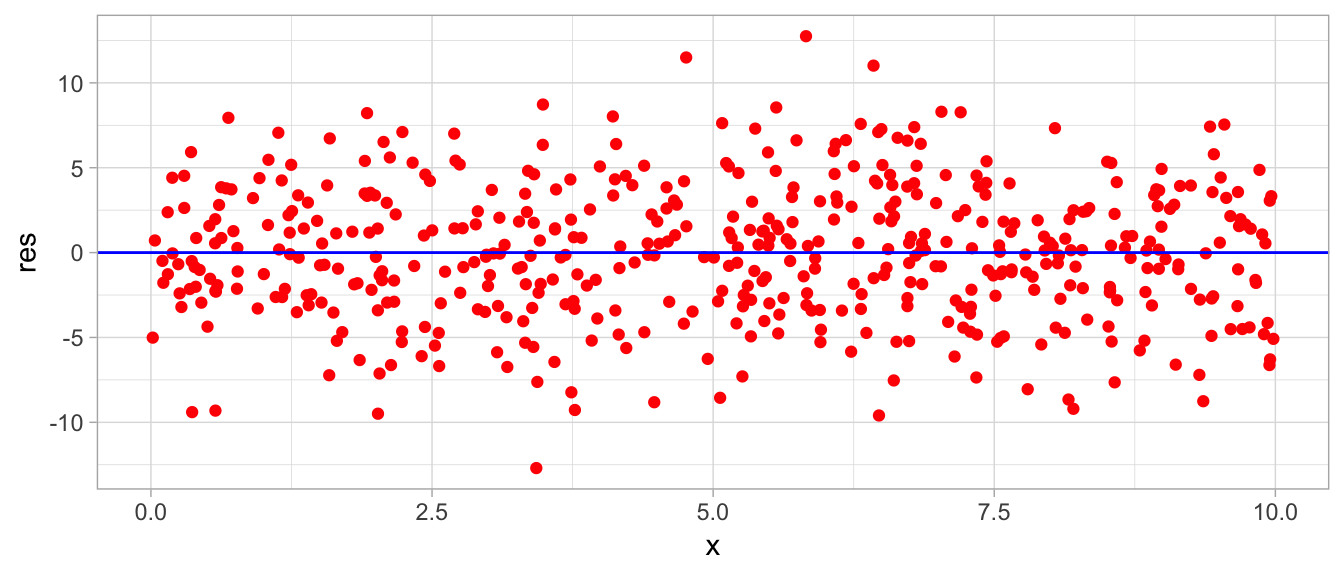
\includegraphics{R4EH_book_files/figure-latex/unnamed-chunk-64-1.pdf}

\section{Regression Output Table}\label{regression-output-table}

The \texttt{broom} package converts \texttt{lm} objects into a tidy
\texttt{data.frame} that can easily be printed in a nice table using
\texttt{knitr}'s \texttt{kable()} function for \texttt{html} output.

\begin{Shaded}
\begin{Highlighting}[]
\CommentTok{# install.packages("broom") # install first if you don't have }
\KeywordTok{library}\NormalTok{(broom)}
\NormalTok{reg2<-}\KeywordTok{tidy}\NormalTok{(my_reg)}
\KeywordTok{kable}\NormalTok{(reg2)}
\end{Highlighting}
\end{Shaded}

\begin{tabular}{l|r|r|r|r}
\hline
term & estimate & std.error & statistic & p.value\\
\hline
(Intercept) & 2.677215 & 0.3695302 & 7.244915 & 0\\
\hline
x & 1.872389 & 0.0642055 & 29.162433 & 0\\
\hline
\end{tabular}

\begin{Shaded}
\begin{Highlighting}[]
\KeywordTok{stargazer}\NormalTok{(my_reg, }\DataTypeTok{type=}\StringTok{"html"}\NormalTok{) }
\end{Highlighting}
\end{Shaded}

Dependent variable:

y

x

1.872***

(0.064)

Constant

2.677***

(0.370)

Observations

500

R2

0.631

Adjusted R2

0.630

Residual Std. Error

4.043 (df = 498)

F Statistic

850.447*** (df = 1; 498)

Note:

\emph{p\textless{}0.1; \textbf{p\textless{}0.05; }}p\textless{}0.01

\chapter{Advanced Regression}\label{advanced-regression}

\textbf{Work in Progress}

Most code is here, but not text explaining everything\ldots{}

\section{Multivariate Regression}\label{multivariate-regression}

\begin{Shaded}
\begin{Highlighting}[]
\KeywordTok{set.seed}\NormalTok{(}\DecValTok{1}\NormalTok{)}
\NormalTok{x<-}\KeywordTok{rnorm}\NormalTok{(}\DecValTok{500}\NormalTok{,}\DecValTok{10}\NormalTok{,}\DecValTok{2}\NormalTok{)}
\NormalTok{z<-}\KeywordTok{runif}\NormalTok{(}\DecValTok{500}\NormalTok{,}\DecValTok{10}\NormalTok{,}\DecValTok{20}\NormalTok{)}
\NormalTok{y<-}\KeywordTok{rnorm}\NormalTok{(}\DecValTok{500}\NormalTok{,}\DecValTok{2}\OperatorTok{*}\NormalTok{x}\OperatorTok{*}\NormalTok{z,}\DecValTok{2}\NormalTok{)}
\NormalTok{year<-}\KeywordTok{sample}\NormalTok{(}\KeywordTok{seq}\NormalTok{(}\DecValTok{2000}\NormalTok{,}\DecValTok{2018}\NormalTok{,}\DecValTok{1}\NormalTok{),}\DecValTok{500}\NormalTok{,}\DataTypeTok{replace=}\OtherTok{TRUE}\NormalTok{)}

\CommentTok{# generate categorical variables}

\CommentTok{# make a shape variable }
\NormalTok{shapes<-}\KeywordTok{c}\NormalTok{(}\StringTok{"square"}\NormalTok{,}\StringTok{"circle"}\NormalTok{,}\StringTok{"triangle"}\NormalTok{,}\StringTok{"rectangle"}\NormalTok{,}\StringTok{"trapezoid"}\NormalTok{)}
\NormalTok{shape<-}\KeywordTok{sample}\NormalTok{(shapes,}\DecValTok{500}\NormalTok{,}\DataTypeTok{replace=}\OtherTok{TRUE}\NormalTok{) }\CommentTok{# sample 500 random draws with replacement from shapes}

\CommentTok{# make a region variable }
\NormalTok{regions<-}\KeywordTok{c}\NormalTok{(}\StringTok{"north"}\NormalTok{,}\StringTok{"south"}\NormalTok{,}\StringTok{"east"}\NormalTok{,}\StringTok{"west"}\NormalTok{)}
\NormalTok{region<-}\KeywordTok{sample}\NormalTok{(regions,}\DecValTok{500}\NormalTok{,}\DataTypeTok{replace=}\OtherTok{TRUE}\NormalTok{) }\CommentTok{# sample 500 random draws with replacement from regions}

\CommentTok{# make a dummy variable }
\NormalTok{yes<-}\KeywordTok{sample}\NormalTok{(}\KeywordTok{c}\NormalTok{(}\DecValTok{0}\NormalTok{,}\DecValTok{1}\NormalTok{),}\DecValTok{500}\NormalTok{,}\DataTypeTok{replace=}\OtherTok{TRUE}\NormalTok{) }

\CommentTok{# combine into dataframe called df}

\NormalTok{df<-}\KeywordTok{data.frame}\NormalTok{(}\DataTypeTok{x=}\NormalTok{x,}
               \DataTypeTok{y=}\NormalTok{y,}
               \DataTypeTok{z=}\NormalTok{z,}
               \DataTypeTok{shape=}\KeywordTok{factor}\NormalTok{(shape),}
               \DataTypeTok{region=}\KeywordTok{factor}\NormalTok{(region),}
               \DataTypeTok{yes=}\NormalTok{yes,}
               \DataTypeTok{year=}\KeywordTok{factor}\NormalTok{(year))}

\CommentTok{# look at new df}

\KeywordTok{head}\NormalTok{(df)}
\end{Highlighting}
\end{Shaded}

\begin{verbatim}
##           x        y        z     shape region yes year
## 1  8.747092 264.8931 15.30809 trapezoid   east   0 2009
## 2 10.367287 347.6574 16.84861  triangle   west   1 2001
## 3  8.328743 227.9193 13.83283    square   east   0 2016
## 4 13.190562 517.0824 19.54988    circle   east   0 2008
## 5 10.659016 235.8301 11.18357 trapezoid  north   1 2018
## 6  8.359063 169.6481 10.39100 trapezoid   west   0 2009
\end{verbatim}

It is quite simply to simply add additional covariates to a regression.
In the \texttt{lm} object, we add variables with \texttt{+}.

\begin{Shaded}
\begin{Highlighting}[]
\NormalTok{reg1<-}\KeywordTok{lm}\NormalTok{(y}\OperatorTok{~}\NormalTok{x}\OperatorTok{+}\NormalTok{z, }\DataTypeTok{data=}\NormalTok{df)}
\KeywordTok{summary}\NormalTok{(reg1)}
\end{Highlighting}
\end{Shaded}

\begin{verbatim}
## 
## Call:
## lm(formula = y ~ x + z, data = df)
## 
## Residuals:
##     Min      1Q  Median      3Q     Max 
## -47.969  -5.115  -0.013   5.756  42.078 
## 
## Coefficients:
##              Estimate Std. Error t value Pr(>|t|)    
## (Intercept) -295.7258     3.7549  -78.76   <2e-16 ***
## x             29.4336     0.2671  110.19   <2e-16 ***
## z             20.1389     0.1849  108.94   <2e-16 ***
## ---
## Signif. codes:  0 '***' 0.001 '**' 0.01 '*' 0.05 '.' 0.1 ' ' 1
## 
## Residual standard error: 12.05 on 497 degrees of freedom
## Multiple R-squared:  0.9809, Adjusted R-squared:  0.9808 
## F-statistic: 1.277e+04 on 2 and 497 DF,  p-value: < 2.2e-16
\end{verbatim}

\section{Dummy Variables}\label{dummy-variables}

\begin{Shaded}
\begin{Highlighting}[]
\NormalTok{reg_d<-}\KeywordTok{lm}\NormalTok{(y}\OperatorTok{~}\NormalTok{yes, }\DataTypeTok{data=}\NormalTok{df)}
\KeywordTok{summary}\NormalTok{(reg_d)}
\end{Highlighting}
\end{Shaded}

\begin{verbatim}
## 
## Call:
## lm(formula = y ~ yes, data = df)
## 
## Residuals:
##      Min       1Q   Median       3Q      Max 
## -199.739  -65.966   -8.196   64.445  272.577 
## 
## Coefficients:
##             Estimate Std. Error t value Pr(>|t|)    
## (Intercept)  296.881      5.324  55.767   <2e-16 ***
## yes            2.588      7.815   0.331    0.741    
## ---
## Signif. codes:  0 '***' 0.001 '**' 0.01 '*' 0.05 '.' 0.1 ' ' 1
## 
## Residual standard error: 87.15 on 498 degrees of freedom
## Multiple R-squared:  0.0002202,  Adjusted R-squared:  -0.001787 
## F-statistic: 0.1097 on 1 and 498 DF,  p-value: 0.7406
\end{verbatim}

The effect on \texttt{y} of going from ``No'' to ``Yes'' is 2.59.

If we wanted to make a dummy variable for an existing categorical
variable

\begin{Shaded}
\begin{Highlighting}[]
\NormalTok{df}\OperatorTok{$}\NormalTok{north<-}\KeywordTok{ifelse}\NormalTok{(region}\OperatorTok{==}\StringTok{"north"}\NormalTok{,}\DecValTok{1}\NormalTok{,}\DecValTok{0}\NormalTok{)}
\NormalTok{df}\OperatorTok{$}\NormalTok{south<-}\KeywordTok{ifelse}\NormalTok{(region}\OperatorTok{==}\StringTok{"south"}\NormalTok{,}\DecValTok{1}\NormalTok{,}\DecValTok{0}\NormalTok{)}
\NormalTok{df}\OperatorTok{$}\NormalTok{east<-}\KeywordTok{ifelse}\NormalTok{(region}\OperatorTok{==}\StringTok{"east"}\NormalTok{,}\DecValTok{1}\NormalTok{,}\DecValTok{0}\NormalTok{)}
\NormalTok{df}\OperatorTok{$}\NormalTok{west<-}\KeywordTok{ifelse}\NormalTok{(region}\OperatorTok{==}\StringTok{"west"}\NormalTok{,}\DecValTok{1}\NormalTok{,}\DecValTok{0}\NormalTok{)}

\KeywordTok{head}\NormalTok{(df)}
\end{Highlighting}
\end{Shaded}

\begin{verbatim}
##           x        y        z     shape region yes year north south east
## 1  8.747092 264.8931 15.30809 trapezoid   east   0 2009     0     0    1
## 2 10.367287 347.6574 16.84861  triangle   west   1 2001     0     0    0
## 3  8.328743 227.9193 13.83283    square   east   0 2016     0     0    1
## 4 13.190562 517.0824 19.54988    circle   east   0 2008     0     0    1
## 5 10.659016 235.8301 11.18357 trapezoid  north   1 2018     1     0    0
## 6  8.359063 169.6481 10.39100 trapezoid   west   0 2009     0     0    0
##   west
## 1    0
## 2    1
## 3    0
## 4    0
## 5    0
## 6    1
\end{verbatim}

Here is where a \texttt{for} loop also can come in handy:

\begin{Shaded}
\begin{Highlighting}[]
\ControlFlowTok{for}\NormalTok{(i }\ControlFlowTok{in} \KeywordTok{unique}\NormalTok{(df}\OperatorTok{$}\NormalTok{region))\{}
\NormalTok{  region[i]<-}\KeywordTok{ifelse}\NormalTok{(df}\OperatorTok{$}\NormalTok{region}\OperatorTok{==}\NormalTok{i,}\DecValTok{1}\NormalTok{,}\DecValTok{0}\NormalTok{)}
\NormalTok{\}}
\end{Highlighting}
\end{Shaded}

\begin{verbatim}
## Warning in region[i] <- ifelse(df$region == i, 1, 0): number of items to
## replace is not a multiple of replacement length

## Warning in region[i] <- ifelse(df$region == i, 1, 0): number of items to
## replace is not a multiple of replacement length

## Warning in region[i] <- ifelse(df$region == i, 1, 0): number of items to
## replace is not a multiple of replacement length

## Warning in region[i] <- ifelse(df$region == i, 1, 0): number of items to
## replace is not a multiple of replacement length
\end{verbatim}

\begin{Shaded}
\begin{Highlighting}[]
\KeywordTok{head}\NormalTok{(df)}
\end{Highlighting}
\end{Shaded}

\begin{verbatim}
##           x        y        z     shape region yes year north south east
## 1  8.747092 264.8931 15.30809 trapezoid   east   0 2009     0     0    1
## 2 10.367287 347.6574 16.84861  triangle   west   1 2001     0     0    0
## 3  8.328743 227.9193 13.83283    square   east   0 2016     0     0    1
## 4 13.190562 517.0824 19.54988    circle   east   0 2008     0     0    1
## 5 10.659016 235.8301 11.18357 trapezoid  north   1 2018     1     0    0
## 6  8.359063 169.6481 10.39100 trapezoid   west   0 2009     0     0    0
##   west
## 1    0
## 2    1
## 3    0
## 4    0
## 5    0
## 6    1
\end{verbatim}

\section{Polynomial Regression}\label{polynomial-regression}

\begin{Shaded}
\begin{Highlighting}[]
\NormalTok{x1<-}\KeywordTok{rnorm}\NormalTok{(}\DecValTok{500}\NormalTok{,}\DecValTok{5}\NormalTok{,}\DecValTok{1}\NormalTok{)}
\NormalTok{y1<-(x1}\OperatorTok{-}\DecValTok{5}\NormalTok{)}\OperatorTok{^}\DecValTok{2}\OperatorTok{+}\DecValTok{2}\OperatorTok{+}\KeywordTok{rnorm}\NormalTok{(}\DecValTok{500}\NormalTok{,}\DecValTok{1}\NormalTok{,}\FloatTok{0.5}\NormalTok{)}

\NormalTok{quad<-}\KeywordTok{data.frame}\NormalTok{(}\DataTypeTok{x=}\NormalTok{x1,}
                 \DataTypeTok{y=}\NormalTok{y1)}
\end{Highlighting}
\end{Shaded}

\begin{Shaded}
\begin{Highlighting}[]
\KeywordTok{library}\NormalTok{(ggplot2)}
\KeywordTok{ggplot}\NormalTok{(quad, }\KeywordTok{aes}\NormalTok{(}\DataTypeTok{x=}\NormalTok{x,}\DataTypeTok{y=}\NormalTok{y))}\OperatorTok{+}
\StringTok{  }\KeywordTok{geom_point}\NormalTok{()}\OperatorTok{+}\KeywordTok{theme_light}\NormalTok{()}
\end{Highlighting}
\end{Shaded}

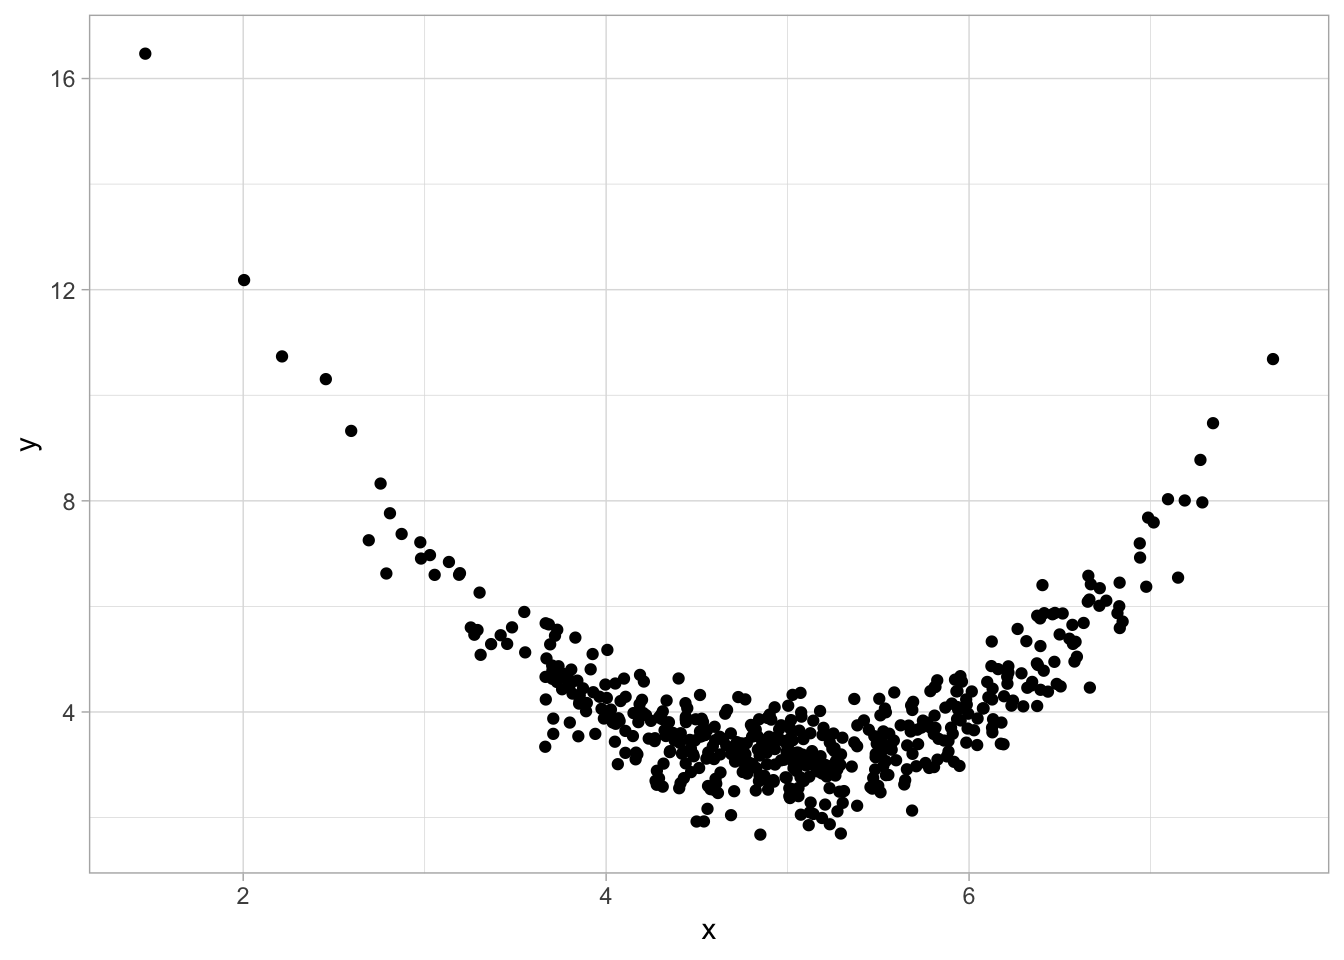
\includegraphics{R4EH_book_files/figure-latex/unnamed-chunk-73-1.pdf}

\begin{Shaded}
\begin{Highlighting}[]
\NormalTok{reg<-}\KeywordTok{lm}\NormalTok{(y}\OperatorTok{~}\NormalTok{x, }\DataTypeTok{data=}\NormalTok{quad)}
\KeywordTok{summary}\NormalTok{(reg)}
\end{Highlighting}
\end{Shaded}

\begin{verbatim}
## 
## Call:
## lm(formula = y ~ x, data = quad)
## 
## Residuals:
##     Min      1Q  Median      3Q     Max 
## -2.3498 -0.8570 -0.3221  0.4573 12.1560 
## 
## Coefficients:
##             Estimate Std. Error t value Pr(>|t|)    
## (Intercept)  4.43961    0.34604   12.83   <2e-16 ***
## x           -0.08518    0.06763   -1.26    0.208    
## ---
## Signif. codes:  0 '***' 0.001 '**' 0.01 '*' 0.05 '.' 0.1 ' ' 1
## 
## Residual standard error: 1.482 on 498 degrees of freedom
## Multiple R-squared:  0.003176,   Adjusted R-squared:  0.001174 
## F-statistic: 1.586 on 1 and 498 DF,  p-value: 0.2084
\end{verbatim}

\begin{Shaded}
\begin{Highlighting}[]
\NormalTok{quadreg<-}\KeywordTok{lm}\NormalTok{(y}\OperatorTok{~}\NormalTok{x}\OperatorTok{+}\KeywordTok{I}\NormalTok{(x}\OperatorTok{^}\DecValTok{2}\NormalTok{), }\DataTypeTok{data=}\NormalTok{quad)}
\KeywordTok{summary}\NormalTok{(quadreg)}
\end{Highlighting}
\end{Shaded}

\begin{verbatim}
## 
## Call:
## lm(formula = y ~ x + I(x^2), data = quad)
## 
## Residuals:
##      Min       1Q   Median       3Q      Max 
## -1.51798 -0.32487  0.01175  0.33870  1.39794 
## 
## Coefficients:
##              Estimate Std. Error t value Pr(>|t|)    
## (Intercept)  28.22753    0.43975   64.19   <2e-16 ***
## x           -10.05640    0.17820  -56.43   <2e-16 ***
## I(x^2)        1.00407    0.01777   56.51   <2e-16 ***
## ---
## Signif. codes:  0 '***' 0.001 '**' 0.01 '*' 0.05 '.' 0.1 ' ' 1
## 
## Residual standard error: 0.5445 on 497 degrees of freedom
## Multiple R-squared:  0.8657, Adjusted R-squared:  0.8652 
## F-statistic:  1602 on 2 and 497 DF,  p-value: < 2.2e-16
\end{verbatim}

\begin{Shaded}
\begin{Highlighting}[]
\KeywordTok{suppressPackageStartupMessages}\NormalTok{(}\KeywordTok{library}\NormalTok{(dplyr))}
\NormalTok{quad<-quad }\OperatorTok
\StringTok{  }\KeywordTok{mutate}\NormalTok{(}\DataTypeTok{x2=}\NormalTok{x}\OperatorTok{^}\DecValTok{2}\NormalTok{,}
         \DataTypeTok{x3=}\NormalTok{x}\OperatorTok{^}\DecValTok{3}\NormalTok{)}

\KeywordTok{head}\NormalTok{(quad)}
\end{Highlighting}
\end{Shaded}

\begin{verbatim}
##          x        y       x2        x3
## 1 6.210004 4.668968 38.56415 239.48352
## 2 4.247019 3.831857 18.03717  76.60422
## 3 4.350733 3.239984 18.92888  82.35448
## 4 4.745756 3.405515 22.52220 106.88484
## 5 3.703630 4.782279 13.71688  50.80225
## 6 4.575343 2.538057 20.93376  95.77914
\end{verbatim}

\begin{Shaded}
\begin{Highlighting}[]
\NormalTok{quadreg2<-}\KeywordTok{lm}\NormalTok{(y}\OperatorTok{~}\NormalTok{x}\OperatorTok{+}\NormalTok{x2, }\DataTypeTok{data=}\NormalTok{quad)}
\KeywordTok{summary}\NormalTok{(quadreg2)}
\end{Highlighting}
\end{Shaded}

\begin{verbatim}
## 
## Call:
## lm(formula = y ~ x + x2, data = quad)
## 
## Residuals:
##      Min       1Q   Median       3Q      Max 
## -1.51798 -0.32487  0.01175  0.33870  1.39794 
## 
## Coefficients:
##              Estimate Std. Error t value Pr(>|t|)    
## (Intercept)  28.22753    0.43975   64.19   <2e-16 ***
## x           -10.05640    0.17820  -56.43   <2e-16 ***
## x2            1.00407    0.01777   56.51   <2e-16 ***
## ---
## Signif. codes:  0 '***' 0.001 '**' 0.01 '*' 0.05 '.' 0.1 ' ' 1
## 
## Residual standard error: 0.5445 on 497 degrees of freedom
## Multiple R-squared:  0.8657, Adjusted R-squared:  0.8652 
## F-statistic:  1602 on 2 and 497 DF,  p-value: < 2.2e-16
\end{verbatim}

Estimating marginal effects.

\begin{Shaded}
\begin{Highlighting}[]
\NormalTok{marginaleffect<-}\ControlFlowTok{function}\NormalTok{(x)\{}
\NormalTok{  quadreg}\OperatorTok{$}\NormalTok{coef[}\DecValTok{2}\NormalTok{]}\OperatorTok{+}\DecValTok{2}\OperatorTok{*}\NormalTok{quadreg}\OperatorTok{$}\NormalTok{coef[}\DecValTok{3}\NormalTok{]}\OperatorTok{*}\NormalTok{x}
\NormalTok{\}}
\KeywordTok{marginaleffect}\NormalTok{(}\DecValTok{1}\OperatorTok{:}\DecValTok{10}\NormalTok{)}
\end{Highlighting}
\end{Shaded}

\begin{verbatim}
##  [1] -8.04826512 -6.04013174 -4.03199837 -2.02386500 -0.01573162
##  [6]  1.99240175  4.00053513  6.00866850  8.01680187 10.02493525
\end{verbatim}

\subsection{Higher Polynomials}\label{higher-polynomials}

\begin{Shaded}
\begin{Highlighting}[]
\NormalTok{cubicreg<-}\KeywordTok{lm}\NormalTok{(y}\OperatorTok{~}\NormalTok{x}\OperatorTok{+}\NormalTok{x2}\OperatorTok{+}\NormalTok{x3, }\DataTypeTok{data=}\NormalTok{quad)}
\KeywordTok{summary}\NormalTok{(cubicreg)}
\end{Highlighting}
\end{Shaded}

\begin{verbatim}
## 
## Call:
## lm(formula = y ~ x + x2 + x3, data = quad)
## 
## Residuals:
##     Min      1Q  Median      3Q     Max 
## -1.5223 -0.3211  0.0116  0.3374  1.3989 
## 
## Coefficients:
##              Estimate Std. Error t value Pr(>|t|)    
## (Intercept) 28.034692   1.102316  25.433  < 2e-16 ***
## x           -9.922597   0.723542 -13.714  < 2e-16 ***
## x2           0.974731   0.154766   6.298 6.65e-10 ***
## x3           0.002049   0.010738   0.191    0.849    
## ---
## Signif. codes:  0 '***' 0.001 '**' 0.01 '*' 0.05 '.' 0.1 ' ' 1
## 
## Residual standard error: 0.545 on 496 degrees of freedom
## Multiple R-squared:  0.8658, Adjusted R-squared:  0.8649 
## F-statistic:  1066 on 3 and 496 DF,  p-value: < 2.2e-16
\end{verbatim}

\begin{Shaded}
\begin{Highlighting}[]
\NormalTok{cubicreg2<-}\KeywordTok{lm}\NormalTok{(y}\OperatorTok{~}\NormalTok{x}\OperatorTok{+}\KeywordTok{I}\NormalTok{(x}\OperatorTok{^}\DecValTok{2}\NormalTok{)}\OperatorTok{+}\KeywordTok{I}\NormalTok{(x}\OperatorTok{^}\DecValTok{3}\NormalTok{), }\DataTypeTok{data=}\NormalTok{quad)}
\KeywordTok{summary}\NormalTok{(cubicreg2)}
\end{Highlighting}
\end{Shaded}

\begin{verbatim}
## 
## Call:
## lm(formula = y ~ x + I(x^2) + I(x^3), data = quad)
## 
## Residuals:
##     Min      1Q  Median      3Q     Max 
## -1.5223 -0.3211  0.0116  0.3374  1.3989 
## 
## Coefficients:
##              Estimate Std. Error t value Pr(>|t|)    
## (Intercept) 28.034692   1.102316  25.433  < 2e-16 ***
## x           -9.922597   0.723542 -13.714  < 2e-16 ***
## I(x^2)       0.974731   0.154766   6.298 6.65e-10 ***
## I(x^3)       0.002049   0.010738   0.191    0.849    
## ---
## Signif. codes:  0 '***' 0.001 '**' 0.01 '*' 0.05 '.' 0.1 ' ' 1
## 
## Residual standard error: 0.545 on 496 degrees of freedom
## Multiple R-squared:  0.8658, Adjusted R-squared:  0.8649 
## F-statistic:  1066 on 3 and 496 DF,  p-value: < 2.2e-16
\end{verbatim}

\begin{Shaded}
\begin{Highlighting}[]
\NormalTok{cubicreg3<-}\KeywordTok{lm}\NormalTok{(y}\OperatorTok{~}\KeywordTok{poly}\NormalTok{(x,}\DecValTok{3}\NormalTok{, }\DataTypeTok{raw=}\OtherTok{TRUE}\NormalTok{), }\DataTypeTok{data=}\NormalTok{quad)}
\KeywordTok{summary}\NormalTok{(cubicreg3)}
\end{Highlighting}
\end{Shaded}

\begin{verbatim}
## 
## Call:
## lm(formula = y ~ poly(x, 3, raw = TRUE), data = quad)
## 
## Residuals:
##     Min      1Q  Median      3Q     Max 
## -1.5223 -0.3211  0.0116  0.3374  1.3989 
## 
## Coefficients:
##                          Estimate Std. Error t value Pr(>|t|)    
## (Intercept)             28.034692   1.102316  25.433  < 2e-16 ***
## poly(x, 3, raw = TRUE)1 -9.922597   0.723542 -13.714  < 2e-16 ***
## poly(x, 3, raw = TRUE)2  0.974731   0.154766   6.298 6.65e-10 ***
## poly(x, 3, raw = TRUE)3  0.002049   0.010738   0.191    0.849    
## ---
## Signif. codes:  0 '***' 0.001 '**' 0.01 '*' 0.05 '.' 0.1 ' ' 1
## 
## Residual standard error: 0.545 on 496 degrees of freedom
## Multiple R-squared:  0.8658, Adjusted R-squared:  0.8649 
## F-statistic:  1066 on 3 and 496 DF,  p-value: < 2.2e-16
\end{verbatim}

Finding the maximum or minimum.

\begin{Shaded}
\begin{Highlighting}[]
\NormalTok{min.x<-(}\OperatorTok{-}\FloatTok{0.5}\OperatorTok{*}\NormalTok{quadreg}\OperatorTok{$}\NormalTok{coef[}\DecValTok{2}\NormalTok{]}\OperatorTok{/}\NormalTok{quadreg}\OperatorTok{$}\NormalTok{coef[}\DecValTok{3}\NormalTok{])}
\NormalTok{min.x}
\end{Highlighting}
\end{Shaded}

\begin{verbatim}
##        x 
## 5.007834
\end{verbatim}

\begin{Shaded}
\begin{Highlighting}[]
\CommentTok{# the predicted value of y at the minimum}
\NormalTok{min.yhat<-quadreg}\OperatorTok{$}\NormalTok{coef[}\DecValTok{1}\NormalTok{]}\OperatorTok{+}\NormalTok{quadreg}\OperatorTok{$}\NormalTok{coef[}\DecValTok{2}\NormalTok{]}\OperatorTok{*}\NormalTok{min.x}\OperatorTok{+}\NormalTok{quadreg}\OperatorTok{$}\NormalTok{coef[}\DecValTok{3}\NormalTok{]}\OperatorTok{*}\NormalTok{min.x}
\NormalTok{min.yhat}
\end{Highlighting}
\end{Shaded}

\begin{verbatim}
## (Intercept) 
##   -17.10504
\end{verbatim}

\texttt{yhat} reaches a minimum of -17.11 when \texttt{x} is 5.01.

\(F\)-test of nonlinearity, \(H_0: \beta_2=\beta_3=0\)

\begin{Shaded}
\begin{Highlighting}[]
\KeywordTok{library}\NormalTok{(car)}
\KeywordTok{linearHypothesis}\NormalTok{(cubicreg, }\KeywordTok{c}\NormalTok{(}\StringTok{"x2"}\NormalTok{,}\StringTok{"x3"}\NormalTok{))}
\end{Highlighting}
\end{Shaded}

\begin{verbatim}
## Linear hypothesis test
## 
## Hypothesis:
## x2 = 0
## x3 = 0
## 
## Model 1: restricted model
## Model 2: y ~ x + x2 + x3
## 
##   Res.Df     RSS Df Sum of Sq      F    Pr(>F)    
## 1    498 1093.99                                  
## 2    496  147.34  2    946.66 1593.4 < 2.2e-16 ***
## ---
## Signif. codes:  0 '***' 0.001 '**' 0.01 '*' 0.05 '.' 0.1 ' ' 1
\end{verbatim}

\section{Logarithmic Models}\label{logarithmic-models}

\begin{Shaded}
\begin{Highlighting}[]
\NormalTok{quad<-quad }\OperatorTok
\StringTok{  }\KeywordTok{mutate}\NormalTok{(}\DataTypeTok{l.x=}\KeywordTok{log}\NormalTok{(x),}
         \DataTypeTok{l.y=}\KeywordTok{log}\NormalTok{(y))}

\KeywordTok{head}\NormalTok{(quad)}
\end{Highlighting}
\end{Shaded}

\begin{verbatim}
##          x        y       x2        x3      l.x       l.y
## 1 6.210004 4.668968 38.56415 239.48352 1.826162 1.5409380
## 2 4.247019 3.831857 18.03717  76.60422 1.446217 1.3433495
## 3 4.350733 3.239984 18.92888  82.35448 1.470344 1.1755685
## 4 4.745756 3.405515 22.52220 106.88484 1.557251 1.2253962
## 5 3.703630 4.782279 13.71688  50.80225 1.309314 1.5649173
## 6 4.575343 2.538057 20.93376  95.77914 1.520682 0.9313989
\end{verbatim}

\begin{Shaded}
\begin{Highlighting}[]
\CommentTok{# linear log model}
\NormalTok{lin_log_reg<-}\KeywordTok{lm}\NormalTok{(y}\OperatorTok{~}\NormalTok{l.x, }\DataTypeTok{data =}\NormalTok{ quad)}
\KeywordTok{summary}\NormalTok{(lin_log_reg)}
\end{Highlighting}
\end{Shaded}

\begin{verbatim}
## 
## Call:
## lm(formula = y ~ l.x, data = quad)
## 
## Residuals:
##     Min      1Q  Median      3Q     Max 
## -2.3562 -0.8767 -0.3256  0.4280 10.6428 
## 
## Coefficients:
##             Estimate Std. Error t value Pr(>|t|)    
## (Intercept)   6.3950     0.4952  12.914  < 2e-16 ***
## l.x          -1.4960     0.3082  -4.854 1.62e-06 ***
## ---
## Signif. codes:  0 '***' 0.001 '**' 0.01 '*' 0.05 '.' 0.1 ' ' 1
## 
## Residual standard error: 1.451 on 498 degrees of freedom
## Multiple R-squared:  0.04518,    Adjusted R-squared:  0.04326 
## F-statistic: 23.56 on 1 and 498 DF,  p-value: 1.619e-06
\end{verbatim}

\begin{Shaded}
\begin{Highlighting}[]
\CommentTok{# log-linear model}
\NormalTok{log_lin_reg<-}\KeywordTok{lm}\NormalTok{(l.y}\OperatorTok{~}\NormalTok{x, }\DataTypeTok{data =}\NormalTok{ quad)}
\KeywordTok{summary}\NormalTok{(log_lin_reg)}
\end{Highlighting}
\end{Shaded}

\begin{verbatim}
## 
## Call:
## lm(formula = l.y ~ x, data = quad)
## 
## Residuals:
##      Min       1Q   Median       3Q      Max 
## -0.82126 -0.18617 -0.03703  0.16323  1.44956 
## 
## Coefficients:
##              Estimate Std. Error t value Pr(>|t|)    
## (Intercept)  1.358081   0.072125  18.829   <2e-16 ***
## x           -0.004126   0.014096  -0.293     0.77    
## ---
## Signif. codes:  0 '***' 0.001 '**' 0.01 '*' 0.05 '.' 0.1 ' ' 1
## 
## Residual standard error: 0.3089 on 498 degrees of freedom
## Multiple R-squared:  0.000172,   Adjusted R-squared:  -0.001836 
## F-statistic: 0.08567 on 1 and 498 DF,  p-value: 0.7699
\end{verbatim}

\begin{Shaded}
\begin{Highlighting}[]
\CommentTok{# log-log model}
\NormalTok{log_log_reg<-}\KeywordTok{lm}\NormalTok{(l.y}\OperatorTok{~}\NormalTok{l.x, }\DataTypeTok{data =}\NormalTok{ quad)}
\KeywordTok{summary}\NormalTok{(log_log_reg)}
\end{Highlighting}
\end{Shaded}

\begin{verbatim}
## 
## Call:
## lm(formula = l.y ~ l.x, data = quad)
## 
## Residuals:
##      Min       1Q   Median       3Q      Max 
## -0.82359 -0.19326 -0.03528  0.15071  1.20178 
## 
## Coefficients:
##             Estimate Std. Error t value Pr(>|t|)    
## (Intercept)  1.68170    0.10432   16.12  < 2e-16 ***
## l.x         -0.21616    0.06492   -3.33 0.000934 ***
## ---
## Signif. codes:  0 '***' 0.001 '**' 0.01 '*' 0.05 '.' 0.1 ' ' 1
## 
## Residual standard error: 0.3056 on 498 degrees of freedom
## Multiple R-squared:  0.02178,    Adjusted R-squared:  0.01981 
## F-statistic: 11.09 on 1 and 498 DF,  p-value: 0.0009342
\end{verbatim}

\begin{Shaded}
\begin{Highlighting}[]
\KeywordTok{suppressPackageStartupMessages}\NormalTok{(}\KeywordTok{library}\NormalTok{(stargazer))}
\KeywordTok{stargazer}\NormalTok{(lin_log_reg, log_lin_reg, log_log_reg, }\DataTypeTok{type=}\StringTok{"html"}\NormalTok{, }\DataTypeTok{column.labels =} \KeywordTok{c}\NormalTok{(}\StringTok{"Linear-Log"}\NormalTok{, }\StringTok{"Log-Linear"}\NormalTok{, }\StringTok{"Log-Log"}\NormalTok{))}
\end{Highlighting}
\end{Shaded}

Dependent variable:

y

l.y

Linear-Log

Log-Linear

Log-Log

(1)

(2)

(3)

l.x

-1.496***

-0.216***

(0.308)

(0.065)

x

-0.004

(0.014)

Constant

6.395***

1.358***

1.682***

(0.495)

(0.072)

(0.104)

Observations

500

500

500

R2

0.045

0.0002

0.022

Adjusted R2

0.043

-0.002

0.020

Residual Std. Error (df = 498)

1.451

0.309

0.306

F Statistic (df = 1; 498)

23.564***

0.086

11.086***

Note:

\emph{p\textless{}0.1; \textbf{p\textless{}0.05; }}p\textless{}0.01

Interpretting the coefficients:

\begin{itemize}
\tightlist
\item
  \textbf{Linear-log model}: a 1\% change in \texttt{x} yields a -149.6
  units change in \texttt{y}
\item
  \textbf{Log-linear model}: a 1 unit change in \texttt{x} yields a 0\%
  change in \texttt{y}
\item
  \textbf{Log-log model}: a 1\% change in \texttt{x} yields a -0.22\%
  change in \texttt{y}
\end{itemize}

\section{Standardizing Variables}\label{standardizing-variables}

Easiest way is to use the \texttt{scale()} command as part of the
\texttt{mutate()} command in \texttt{dplyr}.

\begin{Shaded}
\begin{Highlighting}[]
\KeywordTok{library}\NormalTok{(gapminder)}
\NormalTok{gapminder<-gapminder }\OperatorTok\StringTok{ }
\StringTok{  }\KeywordTok{mutate}\NormalTok{(}\DataTypeTok{s.life=}\KeywordTok{scale}\NormalTok{(lifeExp),}
         \DataTypeTok{s.gdp=}\KeywordTok{scale}\NormalTok{(gdpPercap),}
         \DataTypeTok{s.pop=}\KeywordTok{scale}\NormalTok{(pop))}

\NormalTok{stdreg<-}\KeywordTok{lm}\NormalTok{(s.life}\OperatorTok{~}\NormalTok{s.gdp}\OperatorTok{+}\NormalTok{s.pop, }\DataTypeTok{data=}\NormalTok{gapminder)}
\KeywordTok{summary}\NormalTok{(stdreg)}
\end{Highlighting}
\end{Shaded}

\begin{verbatim}
## 
## Call:
## lm(formula = s.life ~ s.gdp + s.pop, data = gapminder)
## 
## Residuals:
##     Min      1Q  Median      3Q     Max 
## -6.4065 -0.5996  0.1591  0.6357  1.4348 
## 
## Coefficients:
##              Estimate Std. Error t value Pr(>|t|)    
## (Intercept) 1.038e-16  1.959e-02    0.00        1    
## s.gdp       5.858e-01  1.960e-02   29.89  < 2e-16 ***
## s.pop       7.995e-02  1.960e-02    4.08 4.72e-05 ***
## ---
## Signif. codes:  0 '***' 0.001 '**' 0.01 '*' 0.05 '.' 0.1 ' ' 1
## 
## Residual standard error: 0.8085 on 1701 degrees of freedom
## Multiple R-squared:  0.3471, Adjusted R-squared:  0.3463 
## F-statistic: 452.2 on 2 and 1701 DF,  p-value: < 2.2e-16
\end{verbatim}

Interpretting the coefficients:

\begin{itemize}
\tightlist
\item
  A 1 standard deviation change in \texttt{gdpPercap} yields a 0.59
  standard deviation change in \texttt{lifeExp}
\item
  A 1 standard deviation change in \texttt{pop} yields a 0.08 standard
  deviation change in \texttt{lifeExp}
\end{itemize}

\section{Panel Data}\label{panel-data}

\begin{Shaded}
\begin{Highlighting}[]
\KeywordTok{str}\NormalTok{(df)}
\end{Highlighting}
\end{Shaded}

\begin{verbatim}
## 'data.frame':    500 obs. of  11 variables:
##  $ x     : num  8.75 10.37 8.33 13.19 10.66 ...
##  $ y     : num  265 348 228 517 236 ...
##  $ z     : num  15.3 16.8 13.8 19.5 11.2 ...
##  $ shape : Factor w/ 5 levels "circle","rectangle",..: 4 5 3 1 4 4 3 1 2 4 ...
##  $ region: Factor w/ 4 levels "east","north",..: 1 4 1 1 2 4 3 3 1 1 ...
##  $ yes   : num  0 1 0 0 1 0 1 1 0 0 ...
##  $ year  : Factor w/ 19 levels "2000","2001",..: 10 2 17 9 19 10 18 1 4 8 ...
##  $ north : num  0 0 0 0 1 0 0 0 0 0 ...
##  $ south : num  0 0 0 0 0 0 1 1 0 0 ...
##  $ east  : num  1 0 1 1 0 0 0 0 1 1 ...
##  $ west  : num  0 1 0 0 0 1 0 0 0 0 ...
\end{verbatim}

Using \textbf{Least Squares Dummy Variable (LSDV)} approach

\begin{Shaded}
\begin{Highlighting}[]
\NormalTok{reg_fe<-}\KeywordTok{lm}\NormalTok{(y}\OperatorTok{~}\NormalTok{x}\OperatorTok{+}\NormalTok{region, }\DataTypeTok{data =}\NormalTok{ df)}
\KeywordTok{summary}\NormalTok{(reg_fe)}
\end{Highlighting}
\end{Shaded}

\begin{verbatim}
## 
## Call:
## lm(formula = y ~ x + region, data = df)
## 
## Residuals:
##      Min       1Q   Median       3Q      Max 
## -133.702  -46.165   -5.717   49.537  120.099 
## 
## Coefficients:
##             Estimate Std. Error t value Pr(>|t|)    
## (Intercept)   -9.916     14.659  -0.676    0.499    
## x             31.333      1.331  23.536   <2e-16 ***
## regionnorth  -11.107      8.031  -1.383    0.167    
## regionsouth  -12.089      7.968  -1.517    0.130    
## regionwest    -2.195      7.945  -0.276    0.782    
## ---
## Signif. codes:  0 '***' 0.001 '**' 0.01 '*' 0.05 '.' 0.1 ' ' 1
## 
## Residual standard error: 60.02 on 495 degrees of freedom
## Multiple R-squared:  0.5287, Adjusted R-squared:  0.5249 
## F-statistic: 138.8 on 4 and 495 DF,  p-value: < 2.2e-16
\end{verbatim}

De-meaned Method using \texttt{plm} package

\begin{Shaded}
\begin{Highlighting}[]
\KeywordTok{library}\NormalTok{(plm)}
\NormalTok{reg_fe2<-}\KeywordTok{plm}\NormalTok{(y}\OperatorTok{~}\NormalTok{x, }\DataTypeTok{data =}\NormalTok{ df, }\DataTypeTok{index =} \StringTok{"region"}\NormalTok{, }\DataTypeTok{model =} \StringTok{"within"}\NormalTok{)}
\KeywordTok{summary}\NormalTok{(reg_fe2)}
\end{Highlighting}
\end{Shaded}

\begin{verbatim}
## Oneway (individual) effect Within Model
## 
## Call:
## plm(formula = y ~ x, data = df, model = "within", index = "region")
## 
## Unbalanced Panel: n = 4, T = 98-137, N = 500
## 
## Residuals:
##      Min.   1st Qu.    Median   3rd Qu.      Max. 
## -133.7025  -46.1652   -5.7171   49.5375  120.0992 
## 
## Coefficients:
##   Estimate Std. Error t-value  Pr(>|t|)    
## x  31.3333     1.3313  23.536 < 2.2e-16 ***
## ---
## Signif. codes:  0 '***' 0.001 '**' 0.01 '*' 0.05 '.' 0.1 ' ' 1
## 
## Total Sum of Squares:    3778400
## Residual Sum of Squares: 1783000
## R-Squared:      0.5281
## Adj. R-Squared: 0.52428
## F-statistic: 553.946 on 1 and 495 DF, p-value: < 2.22e-16
\end{verbatim}

\subsection{Two Way Fixed Effects}\label{two-way-fixed-effects}

LSDV method

\begin{Shaded}
\begin{Highlighting}[]
\NormalTok{reg_2way_fe<-}\KeywordTok{lm}\NormalTok{(y}\OperatorTok{~}\NormalTok{x}\OperatorTok{+}\NormalTok{region}\OperatorTok{+}\NormalTok{year, }\DataTypeTok{data =}\NormalTok{ df)}
\KeywordTok{summary}\NormalTok{(reg_2way_fe)}
\end{Highlighting}
\end{Shaded}

\begin{verbatim}
## 
## Call:
## lm(formula = y ~ x + region + year, data = df)
## 
## Residuals:
##      Min       1Q   Median       3Q      Max 
## -144.498  -43.865   -3.377   49.134  127.820 
## 
## Coefficients:
##             Estimate Std. Error t value Pr(>|t|)    
## (Intercept)    5.271     20.281   0.260    0.795    
## x             30.875      1.356  22.775   <2e-16 ***
## regionnorth  -11.198      8.199  -1.366    0.173    
## regionsouth  -11.487      8.156  -1.408    0.160    
## regionwest    -1.072      8.096  -0.132    0.895    
## year2001     -26.478     18.142  -1.459    0.145    
## year2002      -3.579     17.490  -0.205    0.838    
## year2003     -18.924     17.587  -1.076    0.282    
## year2004     -22.182     17.521  -1.266    0.206    
## year2005     -11.986     18.819  -0.637    0.524    
## year2006     -22.034     18.293  -1.205    0.229    
## year2007       3.143     18.147   0.173    0.863    
## year2008       2.870     18.262   0.157    0.875    
## year2009     -12.448     18.742  -0.664    0.507    
## year2010     -16.316     17.583  -0.928    0.354    
## year2011      -4.261     17.522  -0.243    0.808    
## year2012      -6.719     19.379  -0.347    0.729    
## year2013     -19.188     19.911  -0.964    0.336    
## year2014       5.420     18.326   0.296    0.768    
## year2015     -14.284     19.692  -0.725    0.469    
## year2016     -11.172     17.851  -0.626    0.532    
## year2017      -7.987     18.493  -0.432    0.666    
## year2018     -19.580     17.895  -1.094    0.274    
## ---
## Signif. codes:  0 '***' 0.001 '**' 0.01 '*' 0.05 '.' 0.1 ' ' 1
## 
## Residual standard error: 60.39 on 477 degrees of freedom
## Multiple R-squared:  0.5402, Adjusted R-squared:  0.519 
## F-statistic: 25.47 on 22 and 477 DF,  p-value: < 2.2e-16
\end{verbatim}

\begin{Shaded}
\begin{Highlighting}[]
\NormalTok{states<-}\KeywordTok{c}\NormalTok{(}\StringTok{"AL"}\NormalTok{,}\StringTok{"AK"}\NormalTok{,}\StringTok{"AZ"}\NormalTok{,}\StringTok{"AR"}\NormalTok{,}\StringTok{"CA"}\NormalTok{,}\StringTok{"CO"}\NormalTok{,}\StringTok{"CT"}\NormalTok{,}\StringTok{"DE"}\NormalTok{,}\StringTok{"FL"}\NormalTok{,}\StringTok{"GA"}\NormalTok{,}\StringTok{"HI"}\NormalTok{,}\StringTok{"ID"}\NormalTok{,}\StringTok{"IL"}\NormalTok{,}\StringTok{"IN"}\NormalTok{,}\StringTok{"IA"}\NormalTok{,}\StringTok{"KS"}\NormalTok{,}\StringTok{"KY"}\NormalTok{,}\StringTok{"LA"}\NormalTok{,}\StringTok{"ME"}\NormalTok{,}\StringTok{"MD"}\NormalTok{,}\StringTok{"MA"}\NormalTok{,}\StringTok{"MI"}\NormalTok{,}\StringTok{"MN"}\NormalTok{,}\StringTok{"MS"}\NormalTok{,}\StringTok{"MO"}\NormalTok{,}\StringTok{"MT"}\NormalTok{,}\StringTok{"NE"}\NormalTok{,}\StringTok{"NV"}\NormalTok{,}\StringTok{"NH"}\NormalTok{,}\StringTok{"NJ"}\NormalTok{,}\StringTok{"NM"}\NormalTok{,}\StringTok{"NY"}\NormalTok{,}\StringTok{"NC"}\NormalTok{,}\StringTok{"ND"}\NormalTok{,}\StringTok{"OH"}\NormalTok{,}\StringTok{"OK"}\NormalTok{,}\StringTok{"OR"}\NormalTok{,}\StringTok{"PA"}\NormalTok{,}\StringTok{"RI"}\NormalTok{,}\StringTok{"SC"}\NormalTok{,}\StringTok{"SD"}\NormalTok{,}\StringTok{"TN"}\NormalTok{,}\StringTok{"TX"}\NormalTok{,}\StringTok{"UT"}\NormalTok{,}\StringTok{"VT"}\NormalTok{,}\StringTok{"VA"}\NormalTok{,}\StringTok{"WA"}\NormalTok{,}\StringTok{"WV"}\NormalTok{,}\StringTok{"WI"}\NormalTok{,}\StringTok{"WY"}\NormalTok{)}

\NormalTok{df<-}\KeywordTok{data.frame}\NormalTok{() }\CommentTok{# make empty dataframe}

\CommentTok{# for each state, generate data, creates dataframe called df_"state" e.g. df_AL, df_AK, etc. }
\ControlFlowTok{for}\NormalTok{(i }\ControlFlowTok{in} \KeywordTok{unique}\NormalTok{(states))\{}
  \KeywordTok{assign}\NormalTok{(}\KeywordTok{paste}\NormalTok{(}\StringTok{"df"}\NormalTok{,i,}\DataTypeTok{sep=}\StringTok{"_"}\NormalTok{),}\KeywordTok{data.frame}\NormalTok{(}\DataTypeTok{state=}\NormalTok{i,}
                \DataTypeTok{year=}\KeywordTok{seq}\NormalTok{(}\DecValTok{2000}\NormalTok{,}\DecValTok{2018}\NormalTok{,}\DecValTok{1}\NormalTok{),}
                \DataTypeTok{x=}\KeywordTok{rnorm}\NormalTok{(}\DecValTok{19}\NormalTok{,}\DecValTok{5}\NormalTok{,}\DecValTok{1}\NormalTok{),}
                \DataTypeTok{y=}\KeywordTok{rnorm}\NormalTok{(}\DecValTok{19}\NormalTok{,}\DecValTok{2}\OperatorTok{*}\NormalTok{(}\KeywordTok{rnorm}\NormalTok{(}\DecValTok{19}\NormalTok{,}\DecValTok{5}\NormalTok{,}\DecValTok{1}\NormalTok{)),}\DecValTok{1}\NormalTok{)) }\CommentTok{# make y approx 2*x }
\NormalTok{  )}
\NormalTok{\}}

\CommentTok{# make list of state dataframes}
\NormalTok{statedfs<-}\KeywordTok{lapply}\NormalTok{(}\KeywordTok{ls}\NormalTok{(}\DataTypeTok{pattern=}\StringTok{"df_"}\NormalTok{),get)}

\CommentTok{# combine state dataframes to df }
\ControlFlowTok{for}\NormalTok{ (i }\ControlFlowTok{in} \KeywordTok{seq_along}\NormalTok{(statedfs))\{}
\NormalTok{  df<-}\KeywordTok{rbind}\NormalTok{(df,statedfs[[i]])}
\NormalTok{\}}

\CommentTok{# remove all individual state dataframes, (e.g. "df_AL") keep only "df"}
\KeywordTok{rm}\NormalTok{(}\DataTypeTok{list=}\KeywordTok{ls}\NormalTok{(}\DataTypeTok{pattern=}\StringTok{"df_"}\NormalTok{))}
\end{Highlighting}
\end{Shaded}

\begin{Shaded}
\begin{Highlighting}[]
\KeywordTok{library}\NormalTok{(}\StringTok{"plm"}\NormalTok{)}
\KeywordTok{pdim}\NormalTok{(df, }\DataTypeTok{index=}\KeywordTok{c}\NormalTok{(}\StringTok{"state"}\NormalTok{,}\StringTok{"year"}\NormalTok{))}
\end{Highlighting}
\end{Shaded}

\begin{verbatim}
## Balanced Panel: n = 50, T = 19, N = 950
\end{verbatim}

\begin{Shaded}
\begin{Highlighting}[]
\NormalTok{reg_2way_fe<-}\KeywordTok{lm}\NormalTok{(y}\OperatorTok{~}\NormalTok{x}\OperatorTok{+}\NormalTok{state}\OperatorTok{+}\KeywordTok{factor}\NormalTok{(year), }\DataTypeTok{data=}\NormalTok{df)}
\KeywordTok{summary}\NormalTok{(reg_2way_fe)}
\end{Highlighting}
\end{Shaded}

\begin{verbatim}
## 
## Call:
## lm(formula = y ~ x + state + factor(year), data = df)
## 
## Residuals:
##     Min      1Q  Median      3Q     Max 
## -5.6800 -1.4700 -0.0804  1.4517  6.7585 
## 
## Coefficients:
##                   Estimate Std. Error t value Pr(>|t|)    
## (Intercept)      11.381998   0.696423  16.344   <2e-16 ***
## x                -0.145891   0.073974  -1.972   0.0489 *  
## stateAL          -0.631120   0.714836  -0.883   0.3775    
## stateAR          -1.259768   0.714804  -1.762   0.0783 .  
## stateAZ          -0.407688   0.714868  -0.570   0.5686    
## stateCA          -0.307402   0.714781  -0.430   0.6673    
## stateCO          -0.752466   0.714726  -1.053   0.2927    
## stateCT          -1.308885   0.714850  -1.831   0.0674 .  
## stateDE          -1.278362   0.714668  -1.789   0.0740 .  
## stateFL          -1.474282   0.714921  -2.062   0.0395 *  
## stateGA          -0.884094   0.714773  -1.237   0.2165    
## stateHI          -0.332327   0.714717  -0.465   0.6421    
## stateIA          -0.595839   0.715165  -0.833   0.4050    
## stateID          -0.547163   0.715739  -0.764   0.4448    
## stateIL          -0.600631   0.714671  -0.840   0.4009    
## stateIN          -0.848554   0.714770  -1.187   0.2355    
## stateKS          -0.286170   0.716084  -0.400   0.6895    
## stateKY          -0.741245   0.715003  -1.037   0.3002    
## stateLA          -0.419623   0.715409  -0.587   0.5577    
## stateMA          -0.298273   0.715053  -0.417   0.6767    
## stateMD          -0.421651   0.714674  -0.590   0.5553    
## stateME          -0.225449   0.714923  -0.315   0.7526    
## stateMI          -0.323392   0.715337  -0.452   0.6513    
## stateMN          -1.409148   0.714844  -1.971   0.0490 *  
## stateMO           0.301812   0.714674   0.422   0.6729    
## stateMS          -0.894070   0.716129  -1.248   0.2122    
## stateMT          -0.401861   0.714677  -0.562   0.5741    
## stateNC          -0.068496   0.714933  -0.096   0.9237    
## stateND          -0.165348   0.715353  -0.231   0.8173    
## stateNE          -0.900076   0.714719  -1.259   0.2082    
## stateNH          -1.110596   0.714850  -1.554   0.1206    
## stateNJ          -1.243386   0.714667  -1.740   0.0822 .  
## stateNM          -1.040089   0.714855  -1.455   0.1460    
## stateNV          -0.617321   0.714782  -0.864   0.3880    
## stateNY          -1.373121   0.715528  -1.919   0.0553 .  
## stateOH          -1.073487   0.714691  -1.502   0.1334    
## stateOK           0.082996   0.715137   0.116   0.9076    
## stateOR          -0.076596   0.714784  -0.107   0.9147    
## statePA          -1.164706   0.714974  -1.629   0.1037    
## stateRI          -0.145688   0.715129  -0.204   0.8386    
## stateSC          -1.228907   0.715302  -1.718   0.0861 .  
## stateSD          -1.082405   0.715272  -1.513   0.1306    
## stateTN          -0.518475   0.715005  -0.725   0.4686    
## stateTX          -0.245084   0.714922  -0.343   0.7318    
## stateUT          -0.166157   0.714669  -0.232   0.8162    
## stateVA          -0.851774   0.714666  -1.192   0.2336    
## stateVT          -1.258232   0.714696  -1.761   0.0787 .  
## stateWA          -1.366209   0.716866  -1.906   0.0570 .  
## stateWI          -0.378345   0.716385  -0.528   0.5975    
## stateWV           0.264818   0.714670   0.371   0.7111    
## stateWY          -1.193296   0.714766  -1.669   0.0954 .  
## factor(year)2001 -0.639847   0.441018  -1.451   0.1472    
## factor(year)2002 -0.206312   0.440886  -0.468   0.6399    
## factor(year)2003  0.272444   0.441398   0.617   0.5372    
## factor(year)2004  0.495971   0.441746   1.123   0.2618    
## factor(year)2005 -0.351603   0.440569  -0.798   0.4250    
## factor(year)2006  0.104295   0.440831   0.237   0.8130    
## factor(year)2007 -0.181204   0.440577  -0.411   0.6810    
## factor(year)2008 -0.109937   0.441432  -0.249   0.8034    
## factor(year)2009  0.071643   0.440802   0.163   0.8709    
## factor(year)2010  0.077712   0.440860   0.176   0.8601    
## factor(year)2011  0.008026   0.440651   0.018   0.9855    
## factor(year)2012 -0.127856   0.440794  -0.290   0.7718    
## factor(year)2013 -0.067184   0.440720  -0.152   0.8789    
## factor(year)2014 -0.257845   0.440685  -0.585   0.5586    
## factor(year)2015 -0.038034   0.440549  -0.086   0.9312    
## factor(year)2016  0.096685   0.441123   0.219   0.8266    
## factor(year)2017  0.094541   0.441374   0.214   0.8304    
## factor(year)2018 -0.778523   0.441417  -1.764   0.0781 .  
## ---
## Signif. codes:  0 '***' 0.001 '**' 0.01 '*' 0.05 '.' 0.1 ' ' 1
## 
## Residual standard error: 2.203 on 881 degrees of freedom
## Multiple R-squared:  0.06812,    Adjusted R-squared:  -0.003807 
## F-statistic: 0.9471 on 68 and 881 DF,  p-value: 0.5995
\end{verbatim}

\begin{Shaded}
\begin{Highlighting}[]
\NormalTok{reg_2way_fe2<-}\KeywordTok{plm}\NormalTok{(y}\OperatorTok{~}\NormalTok{x, }\DataTypeTok{data=}\NormalTok{df, }\DataTypeTok{index=}\KeywordTok{c}\NormalTok{(}\StringTok{"state"}\NormalTok{,}\StringTok{"year"}\NormalTok{), }\DataTypeTok{model=}\StringTok{"within"}\NormalTok{, }\DataTypeTok{effect=}\StringTok{"twoways"}\NormalTok{)}
\KeywordTok{summary}\NormalTok{(reg_2way_fe2)}
\end{Highlighting}
\end{Shaded}

\begin{verbatim}
## Twoways effects Within Model
## 
## Call:
## plm(formula = y ~ x, data = df, effect = "twoways", model = "within", 
##     index = c("state", "year"))
## 
## Balanced Panel: n = 50, T = 19, N = 950
## 
## Residuals:
##      Min.   1st Qu.    Median   3rd Qu.      Max. 
## -5.679977 -1.470018 -0.080427  1.451664  6.758480 
## 
## Coefficients:
##    Estimate Std. Error t-value Pr(>|t|)  
## x -0.145891   0.073974 -1.9722   0.0489 *
## ---
## Signif. codes:  0 '***' 0.001 '**' 0.01 '*' 0.05 '.' 0.1 ' ' 1
## 
## Total Sum of Squares:    4293.6
## Residual Sum of Squares: 4274.7
## R-Squared:      0.0043955
## Adj. R-Squared: -0.07245
## F-statistic: 3.88952 on 1 and 881 DF, p-value: 0.048901
\end{verbatim}

\bibliography{references.bib}


\end{document}
